\documentclass[../../master_thesis_np.tex]{subfiles}
\graphicspath{{./imgs/}}


\begin{document}
	\chapter{Analysis of Structure and Dynamics}

	This chapter focuses on the development of tools to study ensembles of Active Brownian Particles with aligning interactions, and how these tools can be used to study collective behaviors of ABPS systems.

	\section{Analysis Functions}
	%\todo{non chiamerei questa sezione methods, visto che i metodi specifici li descrivi nelle sezioni successive. Potresti chiamarla Analysis functions/tools o Order analysis functions. Oppure integrarle direttamente nei metodi delle varie sezioni.}
	Our investigation in structure and dynamics is based upon a small yet descriptive set of tools that help unveiling how particles spatially organize and how they move.
	
		\subsection{Pair Correlation Function}
		%\todo{per cosa usi questa funzione? descrive in qualche modo il clustering? spiegalo}
		Pair correlation function, \emph{radial distribution function}, or simply $g(r)$ describes particles' density distribution with respect to a reference point in the system.
		Therefore, $g(r)$ is a function only of the separation $r_{ij} = \abs{\vb{r}_i - \vb{r}_j}$ between particles' pairs. 
		It quantifies how particle in an ensemble position one with respect to each other, giving information about the \emph{structure} of the system.
		Here we will use it to get insights about the onset of long range order in the system.
		This function plays a key role in physics of matter since it is possible to measure it in radiation-scattering experiments \cite{hansen90a} and it is often used in cases where, differently from our problem, particles' positions are not directly accessible.
		
		It is possible to derive definitions for $g(r)$ starting from first principles, like phase-space distribution functions, as it is done in \cite{hansen90a}. 
		Here we will use the Dirac's $\delta$-based expression, which is most reliable measure when particles positions are well known,
		\begin{equation}
			\left\langle \frac{1}{N} \sum_{i=1}^{N} \sum_{j=1}^{N}{}' \delta (\mathbf{r} - \mathbf{r}_j + \mathbf{r}_i) \right\rangle = \rho g(r)
		\end{equation}
		where the prime on the summation sign means not counting terms with $i = j$. 
		It is possible to show that the left hand side approaches the value of the overall number density $\rho$ at large distance.
		
		In order to compute $g(r)$ in our simulations, we first need to take distances between all pairs of particles accounting for periodic boundary conditions.
		Then, to simulate the behavior of a sum of deltas, we divide simulation space in bins by radius, where the area of each bin is computed as the intersection between a circular crown and a square, to respect the geometry of our simulation box without introducing biases.
		After counting the number of particles in each bin, we normalize by the average density to make $g(r) \to 1$ at long distance.
		%\todo{questa è una pratica comune e accettata? perché non normalizzare sulla densità media?}
		
		\subsection{Cluster Size}
		%\todo{sposterei questa prima della polarizzazione}
		As discussed in section \ref{literature}, ensembles of ABPs tend to cluster when an attractive interaction is present or conditions (velocity, packing fraction) are right for MIPS to occur. 
		In most cases, particles form one big cluster while some of them remain in a gaseous phase outside of said cluster. 
		The way system form a big cluster is often through the formation of small clusters throughout the simulation box. These small clusters are dynamic in the size and stable enough to observe for long time periods.
		
		It is possible to extract some information about small clusters from the $g(r)$, however, it is more suited for global structure formation study than for the local cluster formation.
		In order to get some insight about partial clustering, we developed the cluster size analysis. 
		
		Our method was built using DBSCAN \cite{ester_density-based_1996}, a density-based clustering algorithm, which was originally created for data-science but, with the right parameters, can become useful for physics. 
		DBSCAN starts from a point and adds to the cluster associated with that point all the others which are at a distance of less than a threshold. 
		A point having more than $Mp$ points in its vicinity is said \emph{core point} or \emph{seed}. 
		A point in the vicinity of a \emph{core point} is a \emph{border point}. 
		All the others are \emph{noise points}. 
		Using $1$ as $Mp$ (i.e.\ a cluster must be formed with at least 2 points) and particle radius or interactions range as threshold distance, this algorithm's results correspond to the common sense conception of what a cluster is.
		In our case, we used \SI{5}{\um} as threshold distance, enough to join contacting particles with $0.5R$ tolerance, but restricting to one layer of particles in contact, in order to consider only continuous groups as clusters.
		The advantage of adapting an existing algorithm is that it has some very fast pre-built implementations which are probably more efficient than one could write from scratch.
		
		\begin{figure}[htp]
			\centering
			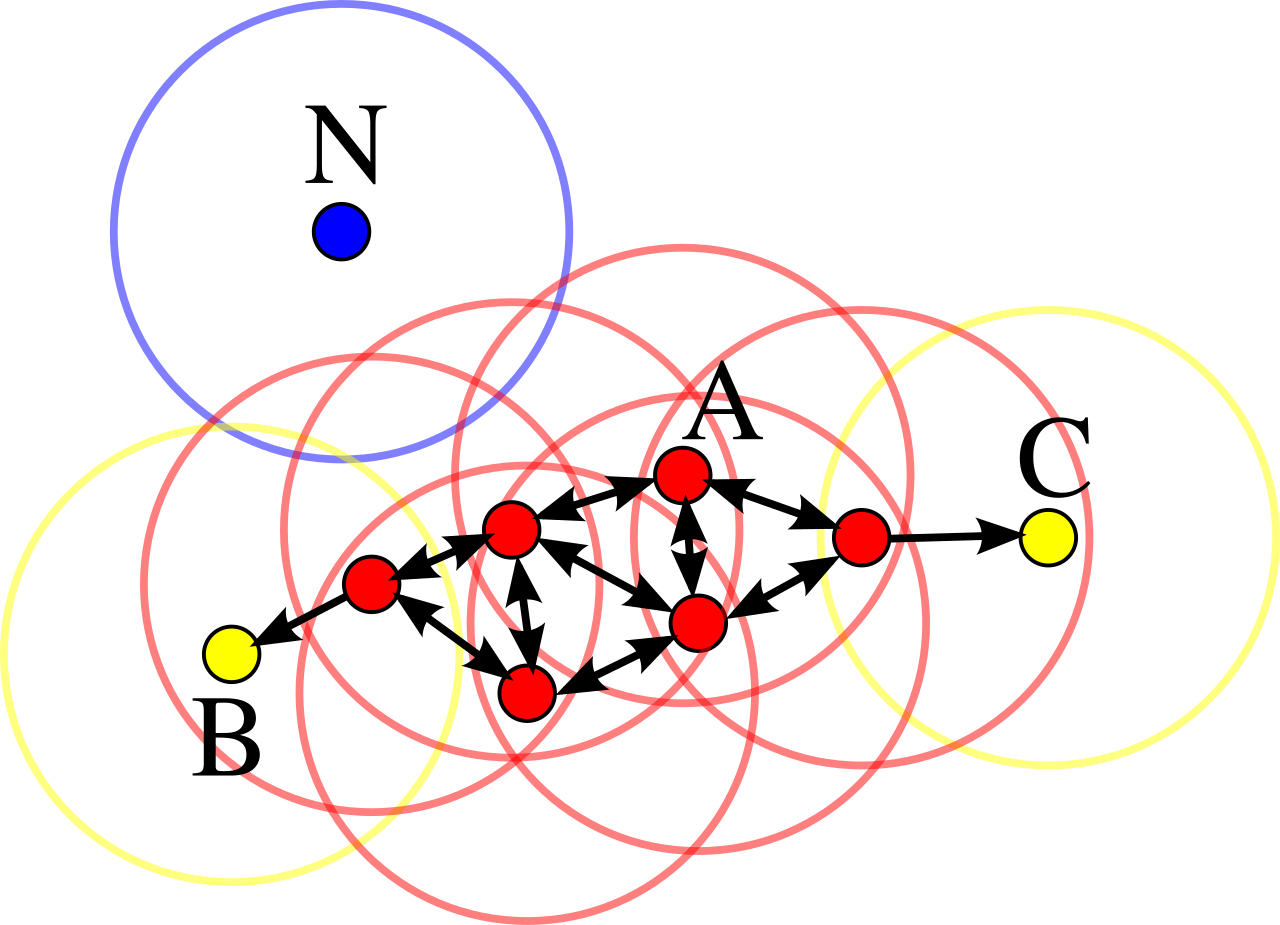
\includegraphics[width=.75\textwidth]{dbscan.png}
			\caption{\enquote{Illustration of DBSCAN cluster analysis (minPts=3). Points around A are core points. Points B and C are not core points, but are density-connected via the cluster of A (and thus belong to this cluster). Point N is Noise, since it is neither a core point nor reachable from a core point}. \cite{chire_deutsch_2011}.}
			\label{fig:dbscan}
		\end{figure}
		
		\subsection{Local and Global Polarization}
		%\todo{sposterei questa più avanti, facendo un'unica sezione di Global and local polarization}
		Whenever the agents of a system have a directed motion, as is the case for ABPs, it is worthwhile to analyze the order in the orientation degree of freedom of agents.  
		
		For global polarization, we use the following definition \cite{caprini_spontaneous_2020}
		\begin{equation}
			P = \frac{1}{N} \abs{\sum_{k=1}^{N} e^{i \theta_k(t)}} 
		\end{equation}
		where $\theta_k$ is the orientation of $k$-th particle. 
		This parameter is $1$ when all particles are aligned and $0$ when they are pointing in random directions. 
		
		In the phase transition section we will use the polarization susceptivity $\chi(P) = N_P(\langle P^2 \rangle - \langle P \rangle^2)$.
		For phase transition like the one we analyze, from disordered to flocking phase, the susceptivity of an order parameter has a peak in the proximity of the critical value for the transition, in this case, the orientational coupling parameter.
		\subsection{Local Polarization}
		As explained in previous section, local properties could provide crucial information about the emergence and properties of global self-organization in the system. 
		When aligning interactions are present and packing fraction is small or we are in a transient, small clusters of particles tend to align their directions, which in terms of global polarization order parameter would correspond to a disordered state, i.e. $P = 0$. 
		We can exploit the fact that clustering algorithms assign points to clusters and then measure how polarized the single groups are, meaning we compute a local polarization order parameter. 
		Averaging over clusters, this parameter $\bar{P}$ will be close to $1$ even if $P$ is kept low by the different orientations of clusters, making it a good parameter to study local properties and short range interactions.
		
		\section{Flocking as a Phase Transition} \label{phasetrans}
		As mentioned in section \ref{literature}, \citeauthor{martin-gomez_collective_2018}, as well as \citeauthor{negi_emergent_2022} \cite{martin-gomez_collective_2018, negi_emergent_2022} showed how inserting an explicitly aligning interaction in the simulation can make the whole system polarize, meaning all particles move in the same direction. 
		This phenomenon is called \emph{flocking}.
		
		\begin{figure}[htp]
			\centering
			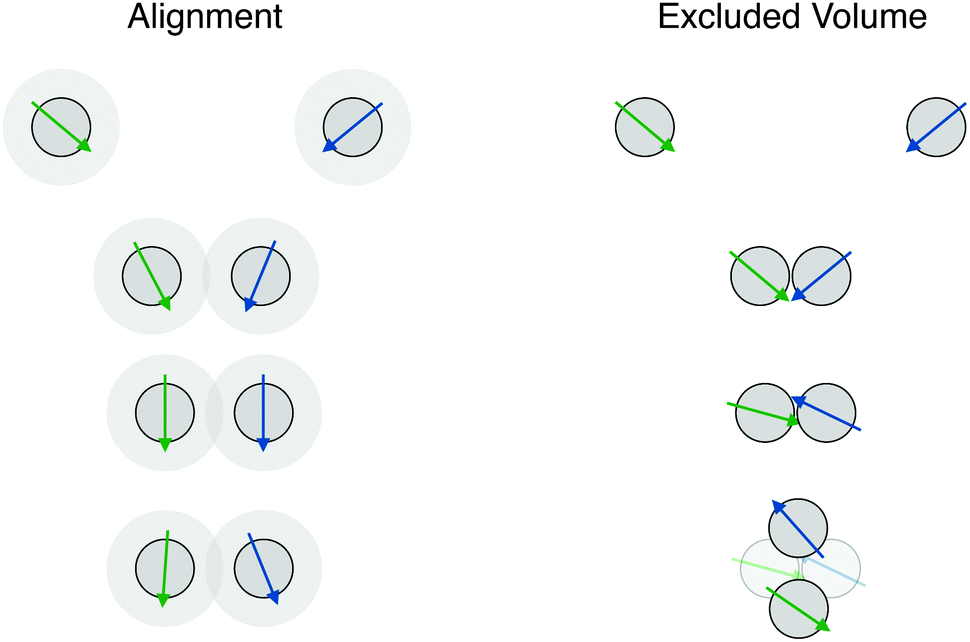
\includegraphics[width=\textwidth]{alignment.png}
			\caption{Behavior of two particles with explicitly aligning interactions, compared with excluded volume steric interaction only. Adapted from \cite{martin-gomez_collective_2018}.}
			\label{fig:alignment}
		\end{figure}
		%\todo{questa figura è presa dal loro paper? le interazioni allineanti sono esplicite? spiega meglio}	
		
		In Figure \ref{fig:alignment}, an example of how the alignment process works. 
		The interaction used by \citeauthor{martin-gomez_collective_2018} is an explicitly aligning torque where $T \sim \sin( \theta_{i}-\theta_{j} )$, with particles orientation are \emph{explicitly} included in the expression and $\abs{T}$ has a minimum where $\theta_{i} = \theta_{j}$~\cite{martin-gomez_collective_2018}. 
		
		Differently from their case, here we show how a repulsive off-centered interaction, although with limited range, can lead an ABPs system to reach a flocking state. 
		The selected interaction force is $F(r) = kr^{-2}$, akin to a Coulomb or gravitational force, where $k$ is a constant. 
		When both the off-center magnitude $\alpha$ and the constant $k$ have a positive value, front sides of interacting particles repel each other, meaning that two particle swimming towards each other will tend to align their orientations. 
		Our alignment thus comes automatically from applying a force to a non centered position. 
		In Figure \ref{fig:flock40}\, an example of how flocking transition happens in our simulations with $k = 10$, with an interaction range of \SI{40}{\micro\meter}.

		\begin{figure}[hbtp]
			\centering
			\subfloat{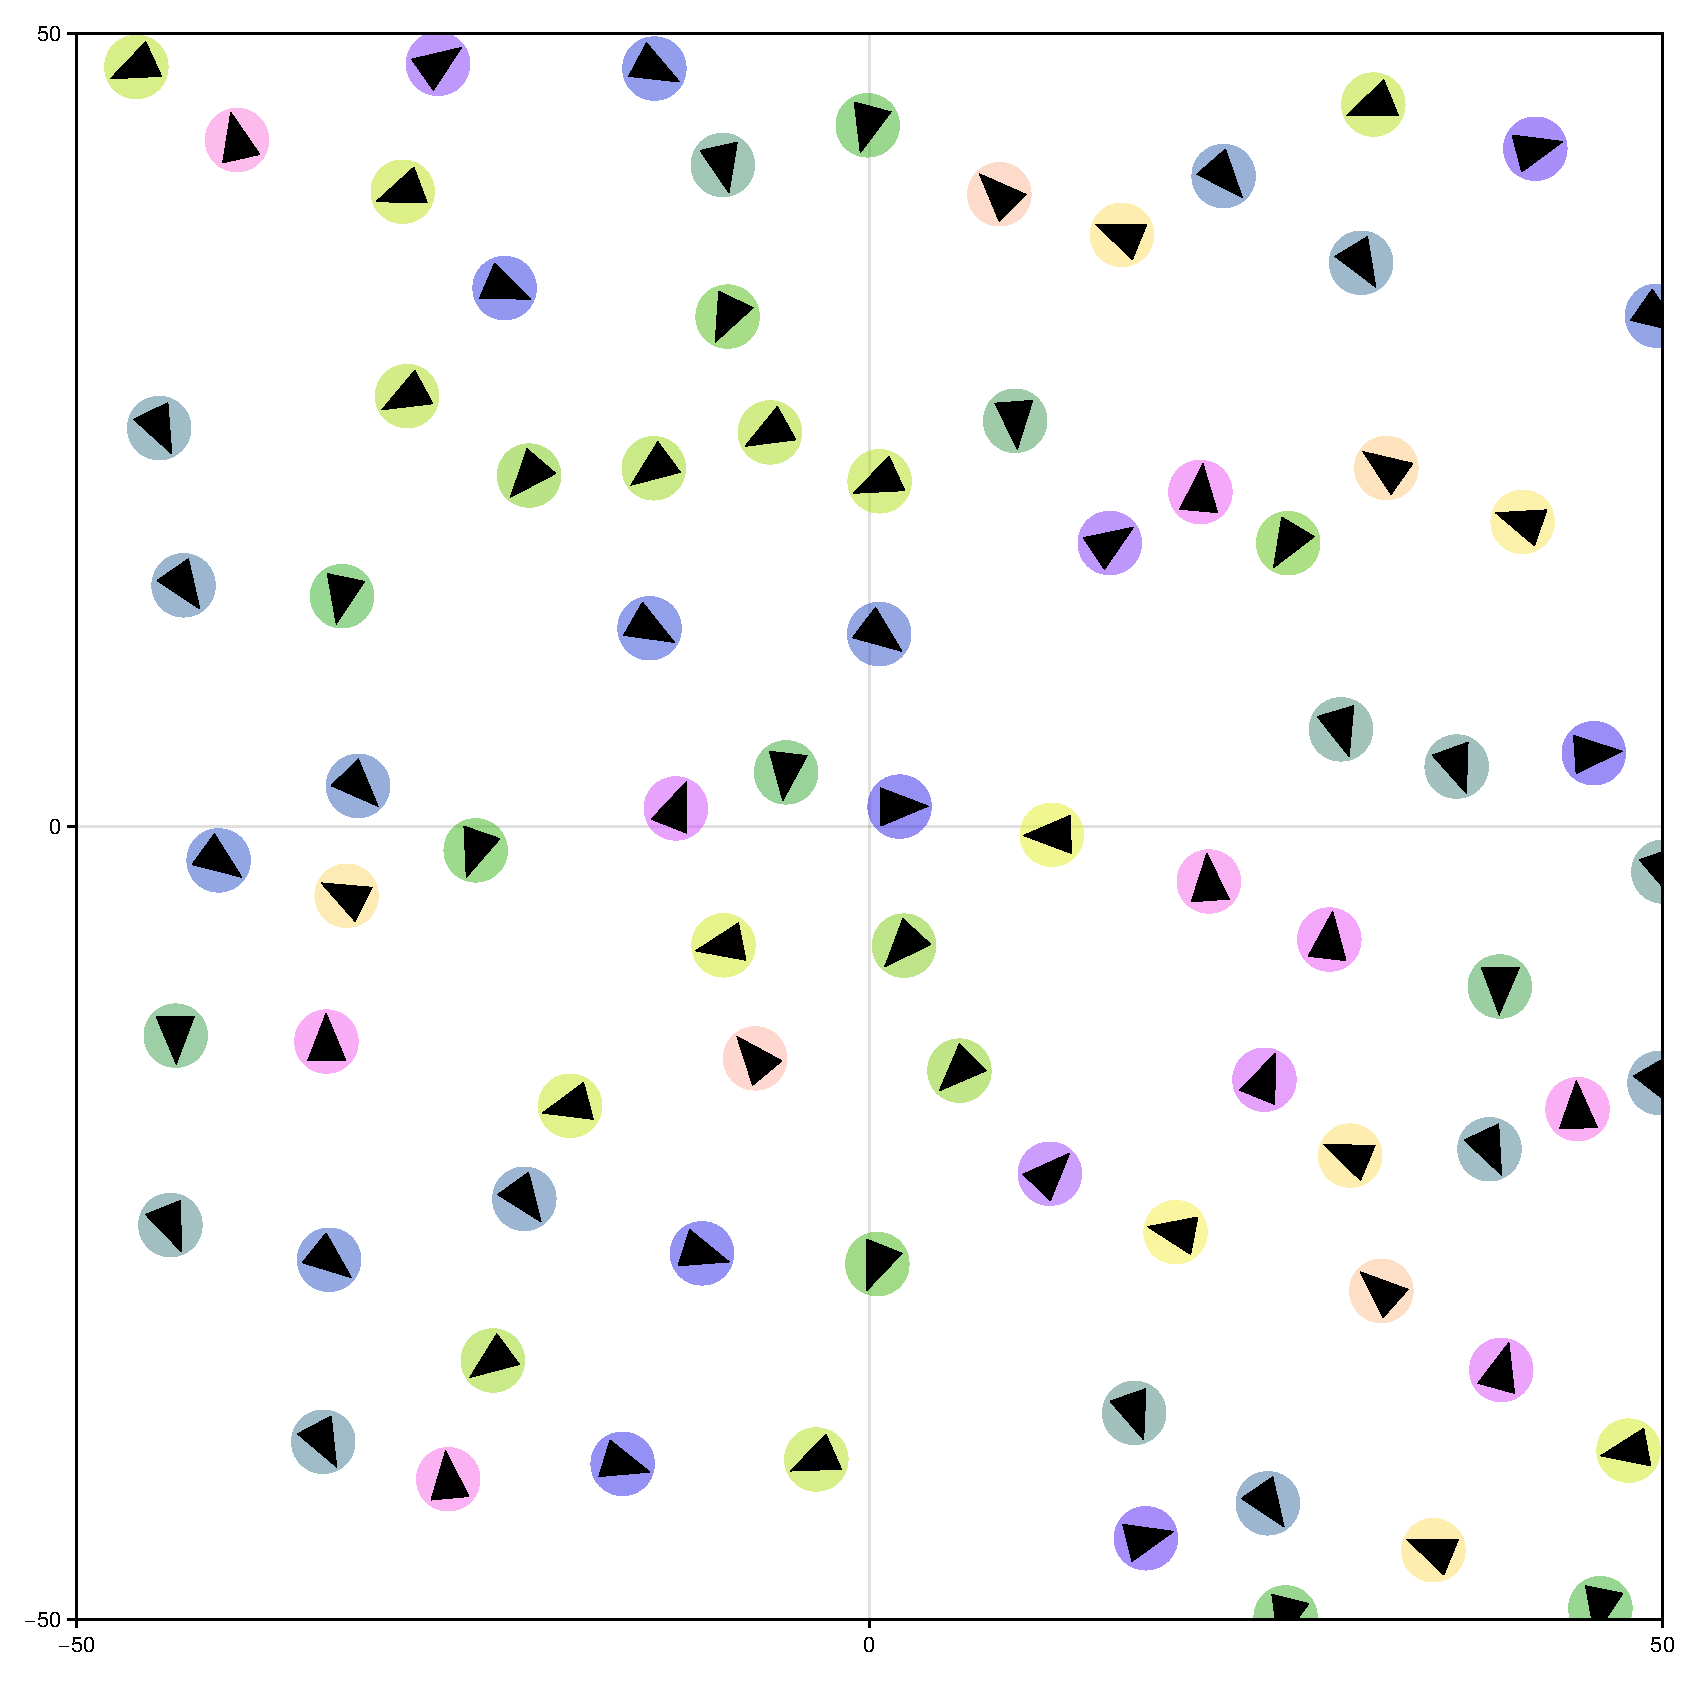
\includegraphics[width=.33\textwidth]{coulombrange40/flocking_1.0s.pdf}}
			\subfloat{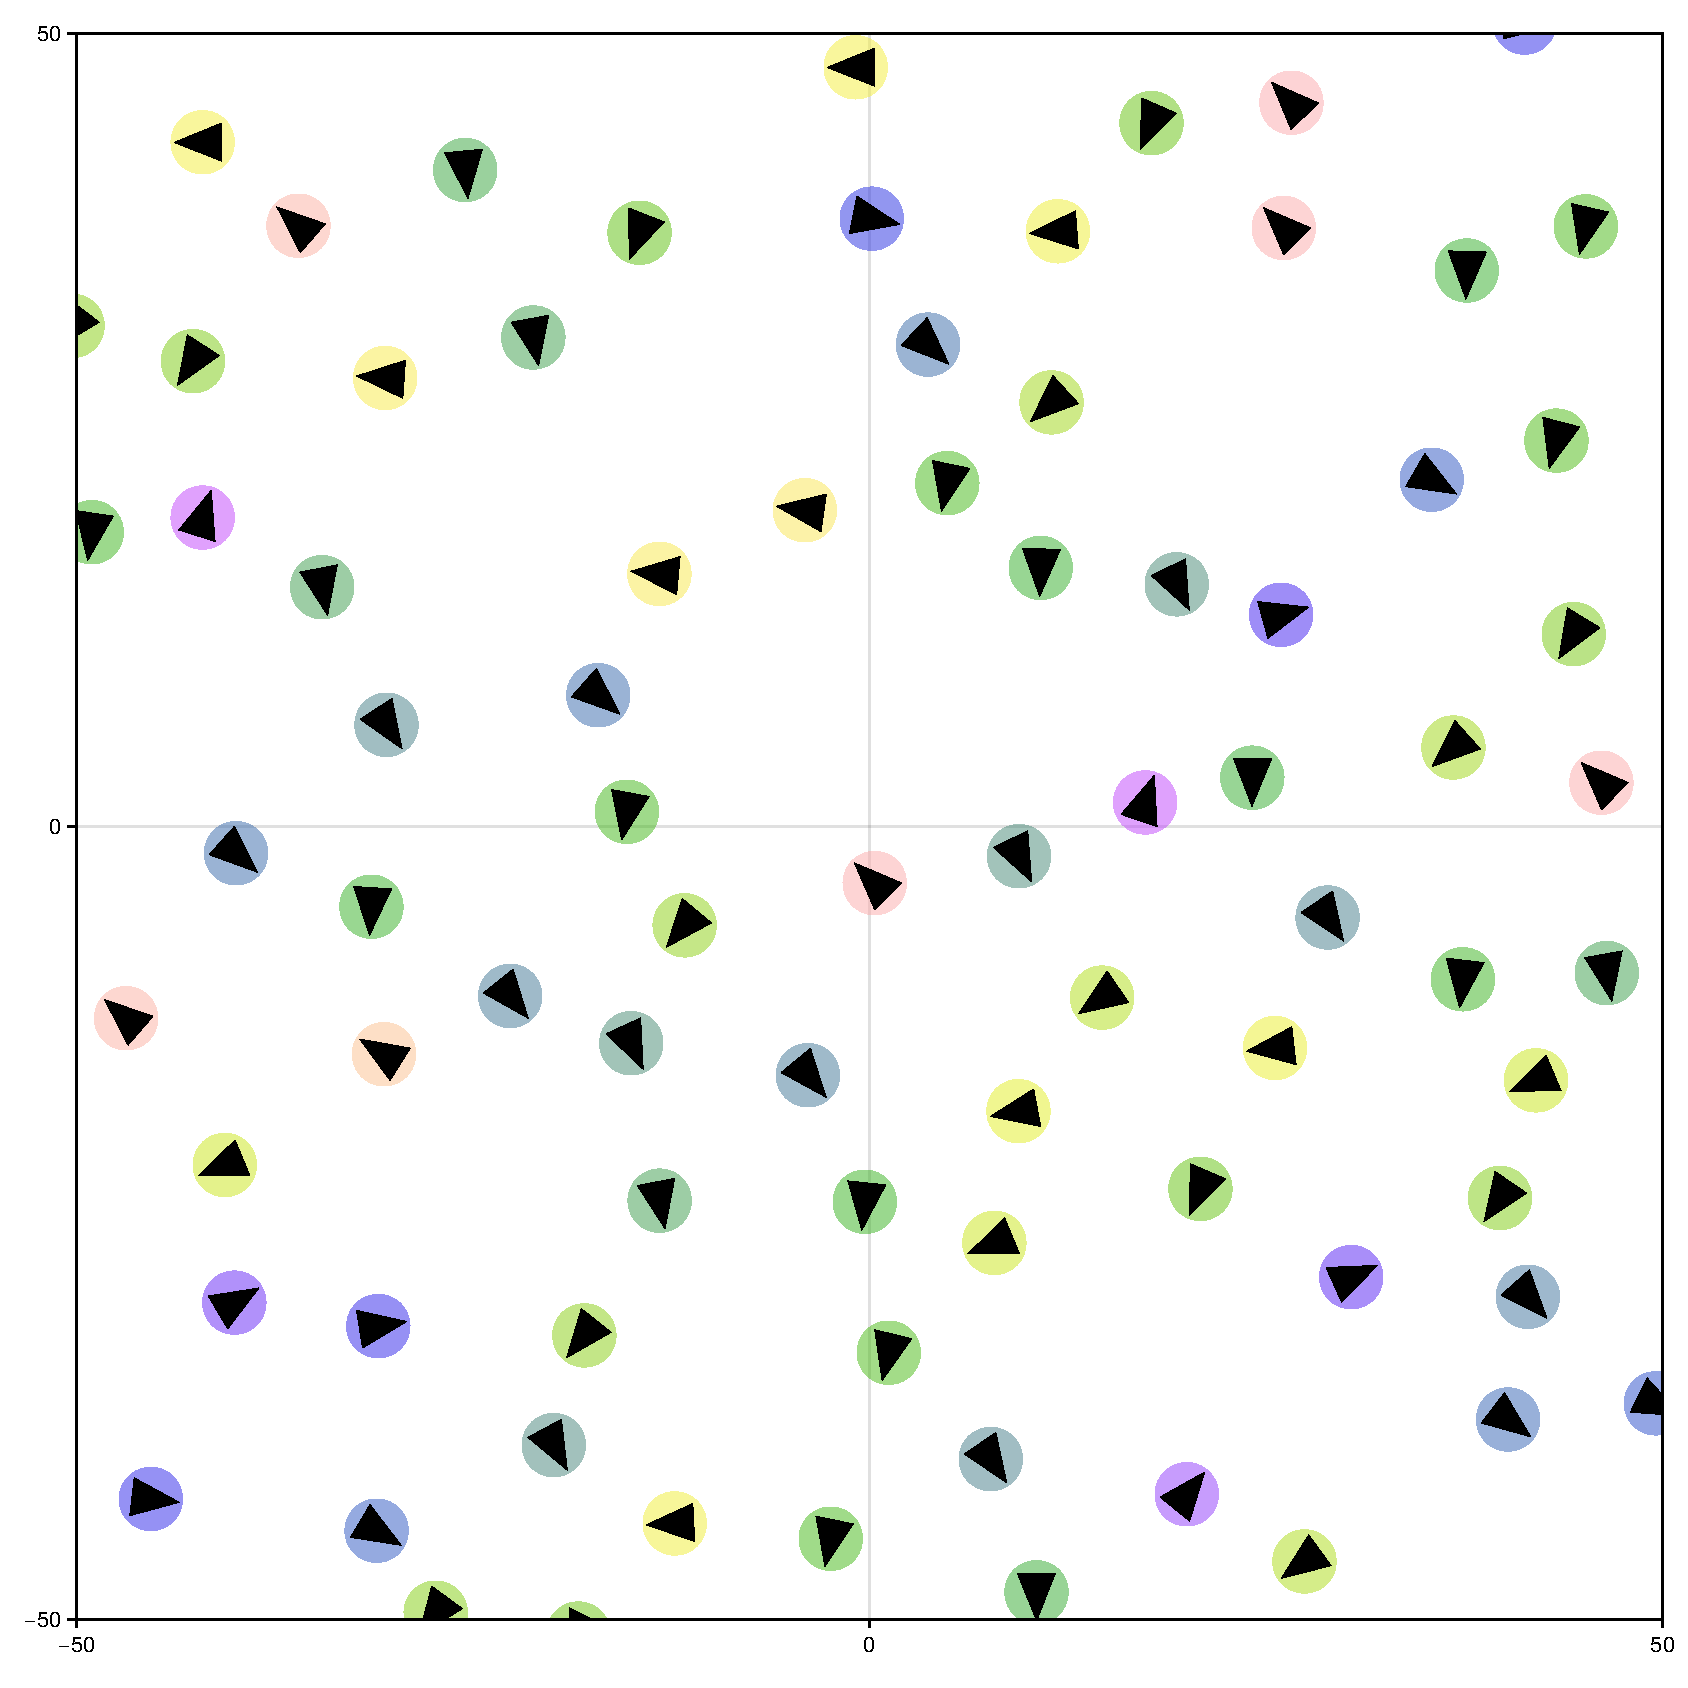
\includegraphics[width=.33\textwidth]{coulombrange40/flocking_5.0s.pdf}}
			\subfloat{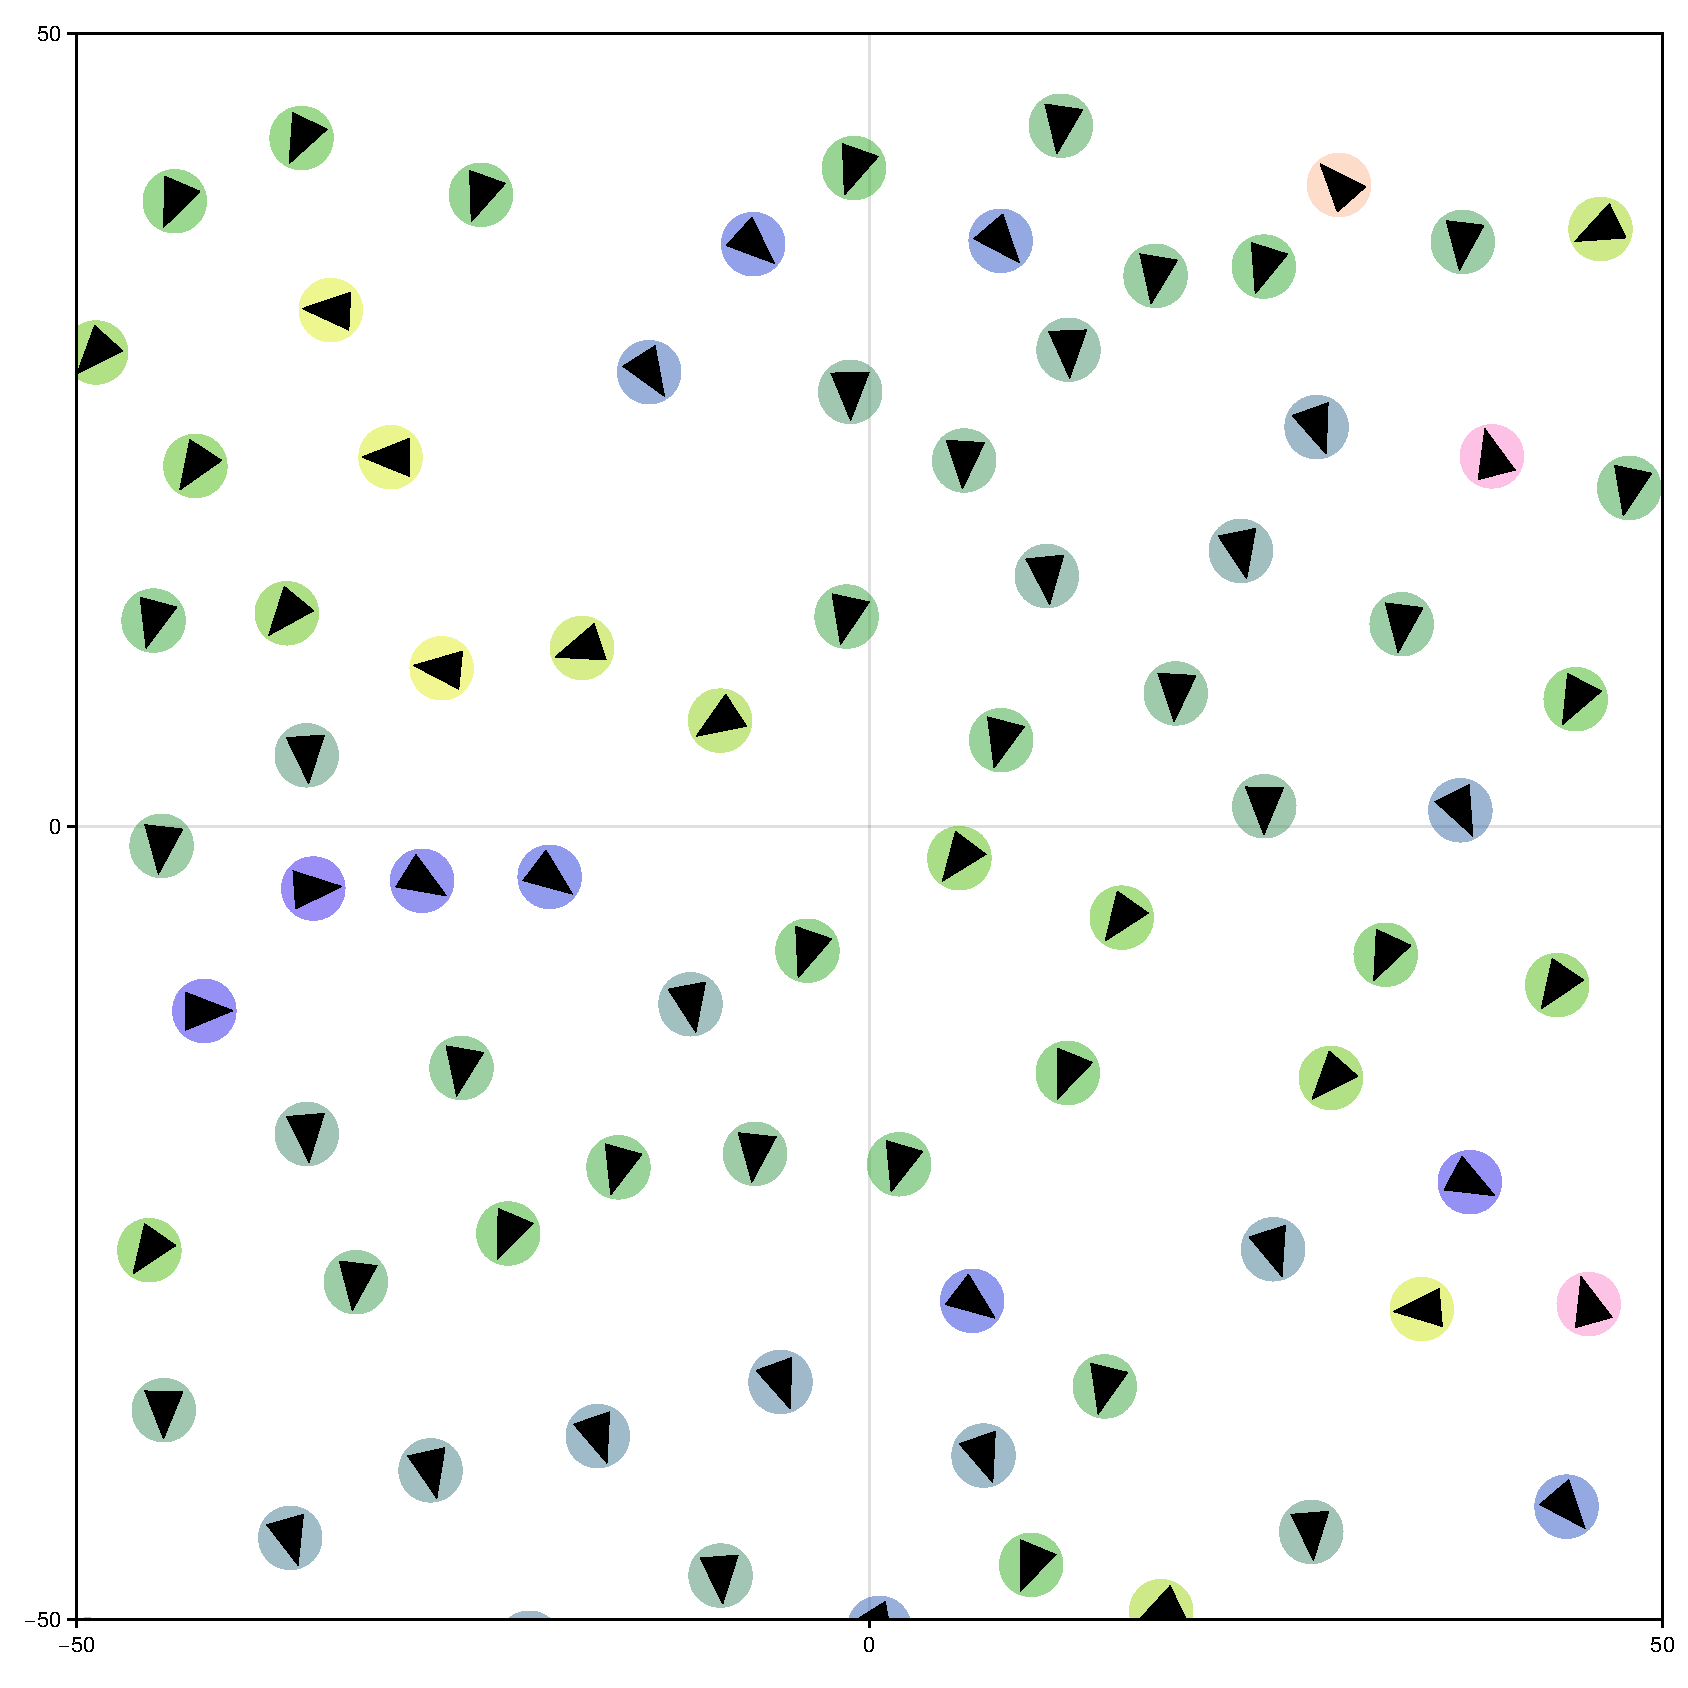
\includegraphics[width=.33\textwidth]{coulombrange40/flocking_10.0s.pdf}}\\
			\subfloat{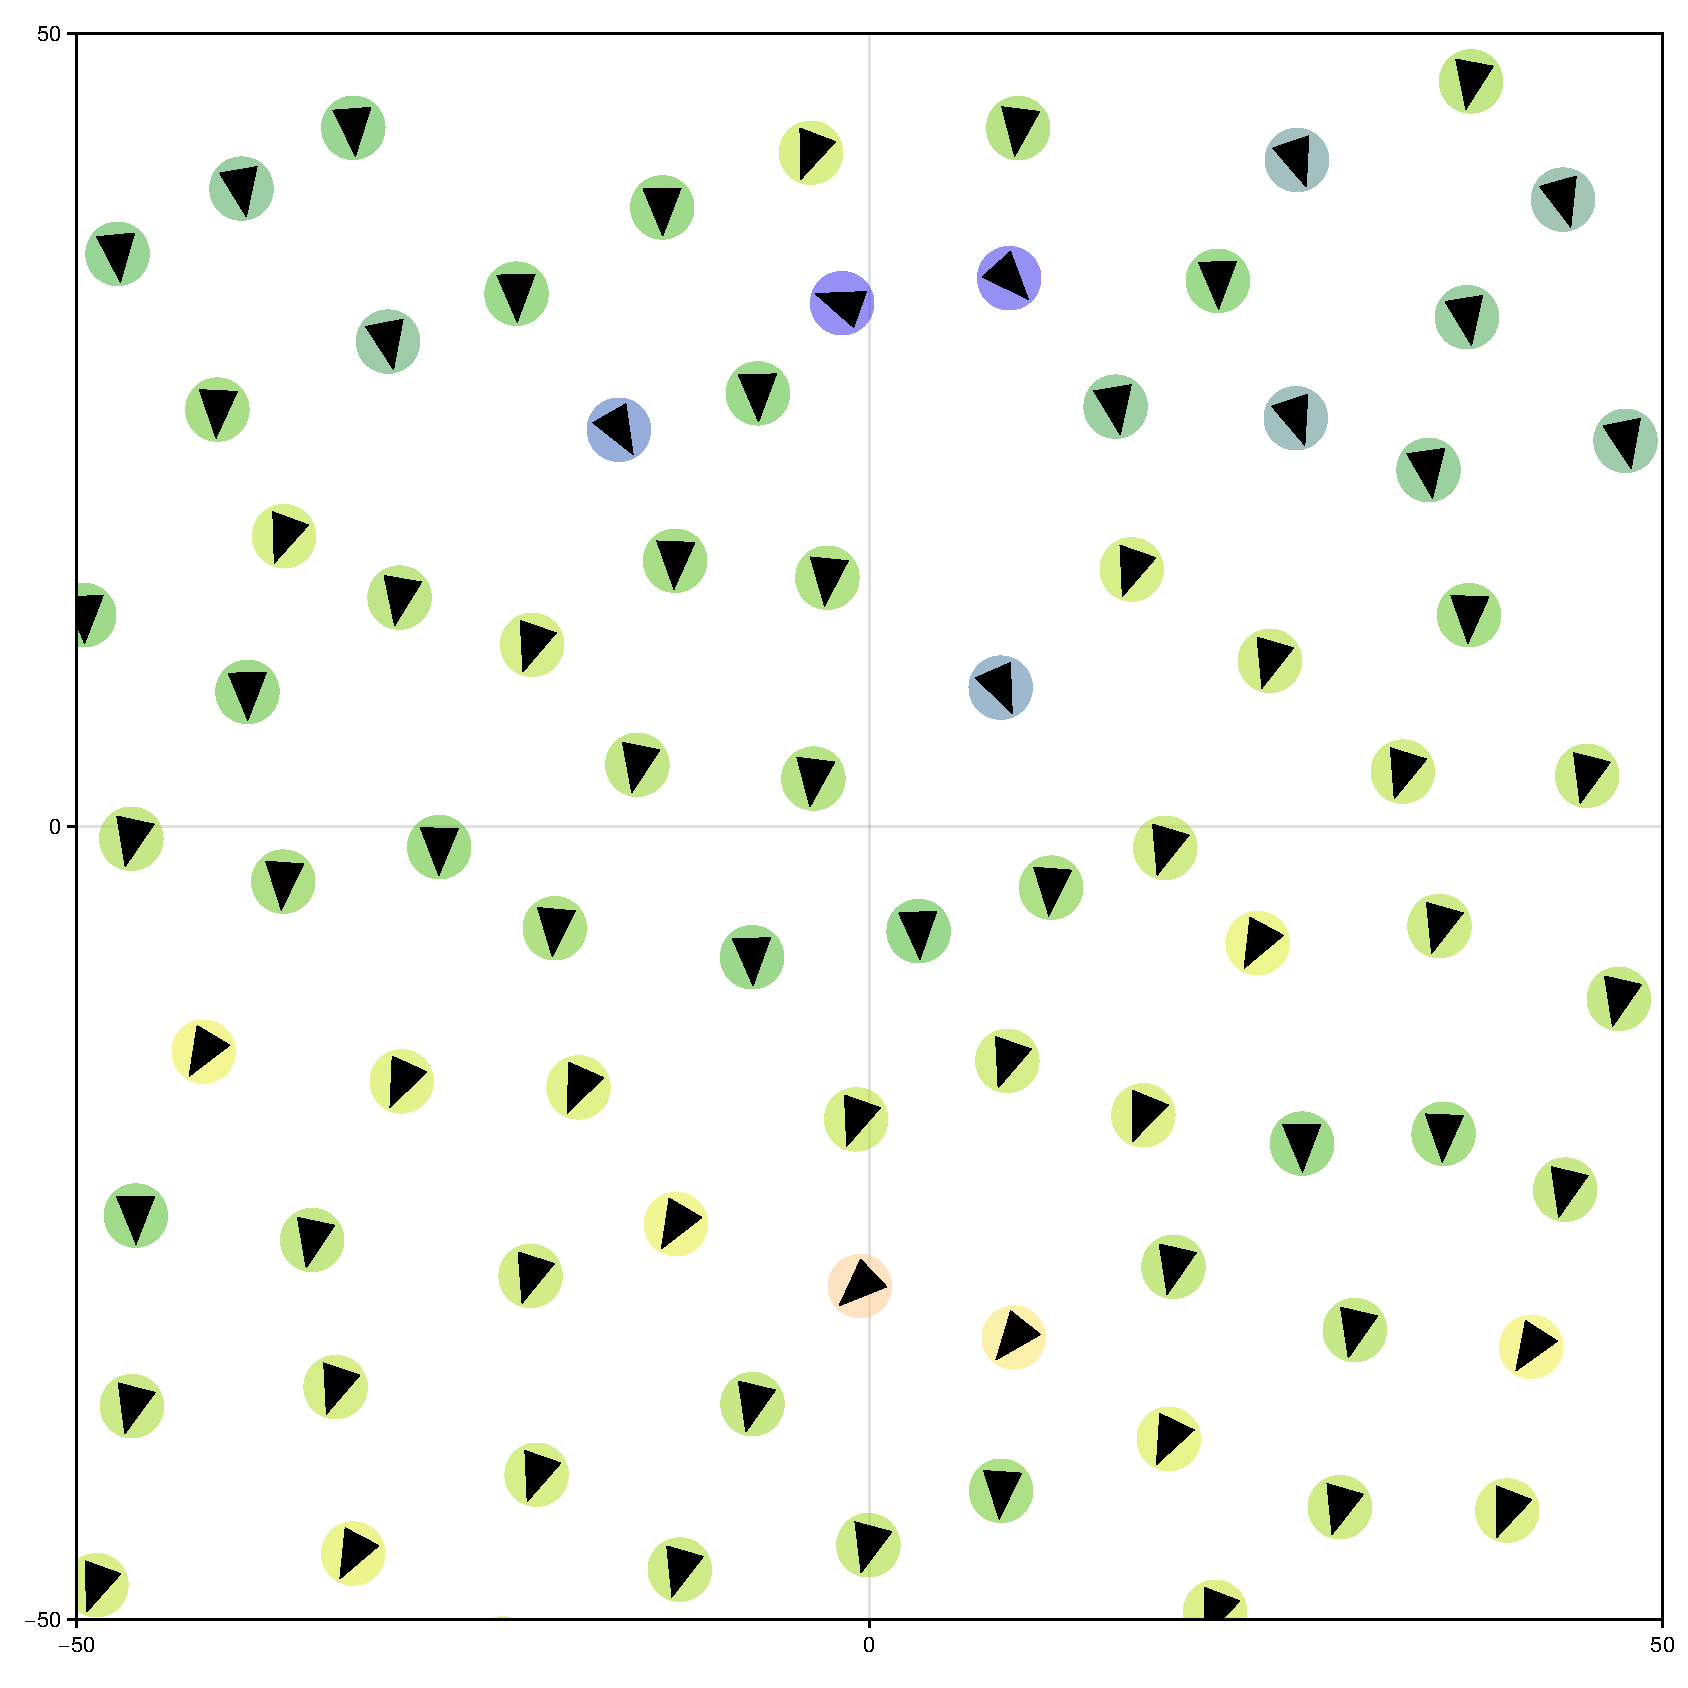
\includegraphics[width=.33\textwidth]{coulombrange40/flocking_15.0s.pdf}}
			\subfloat{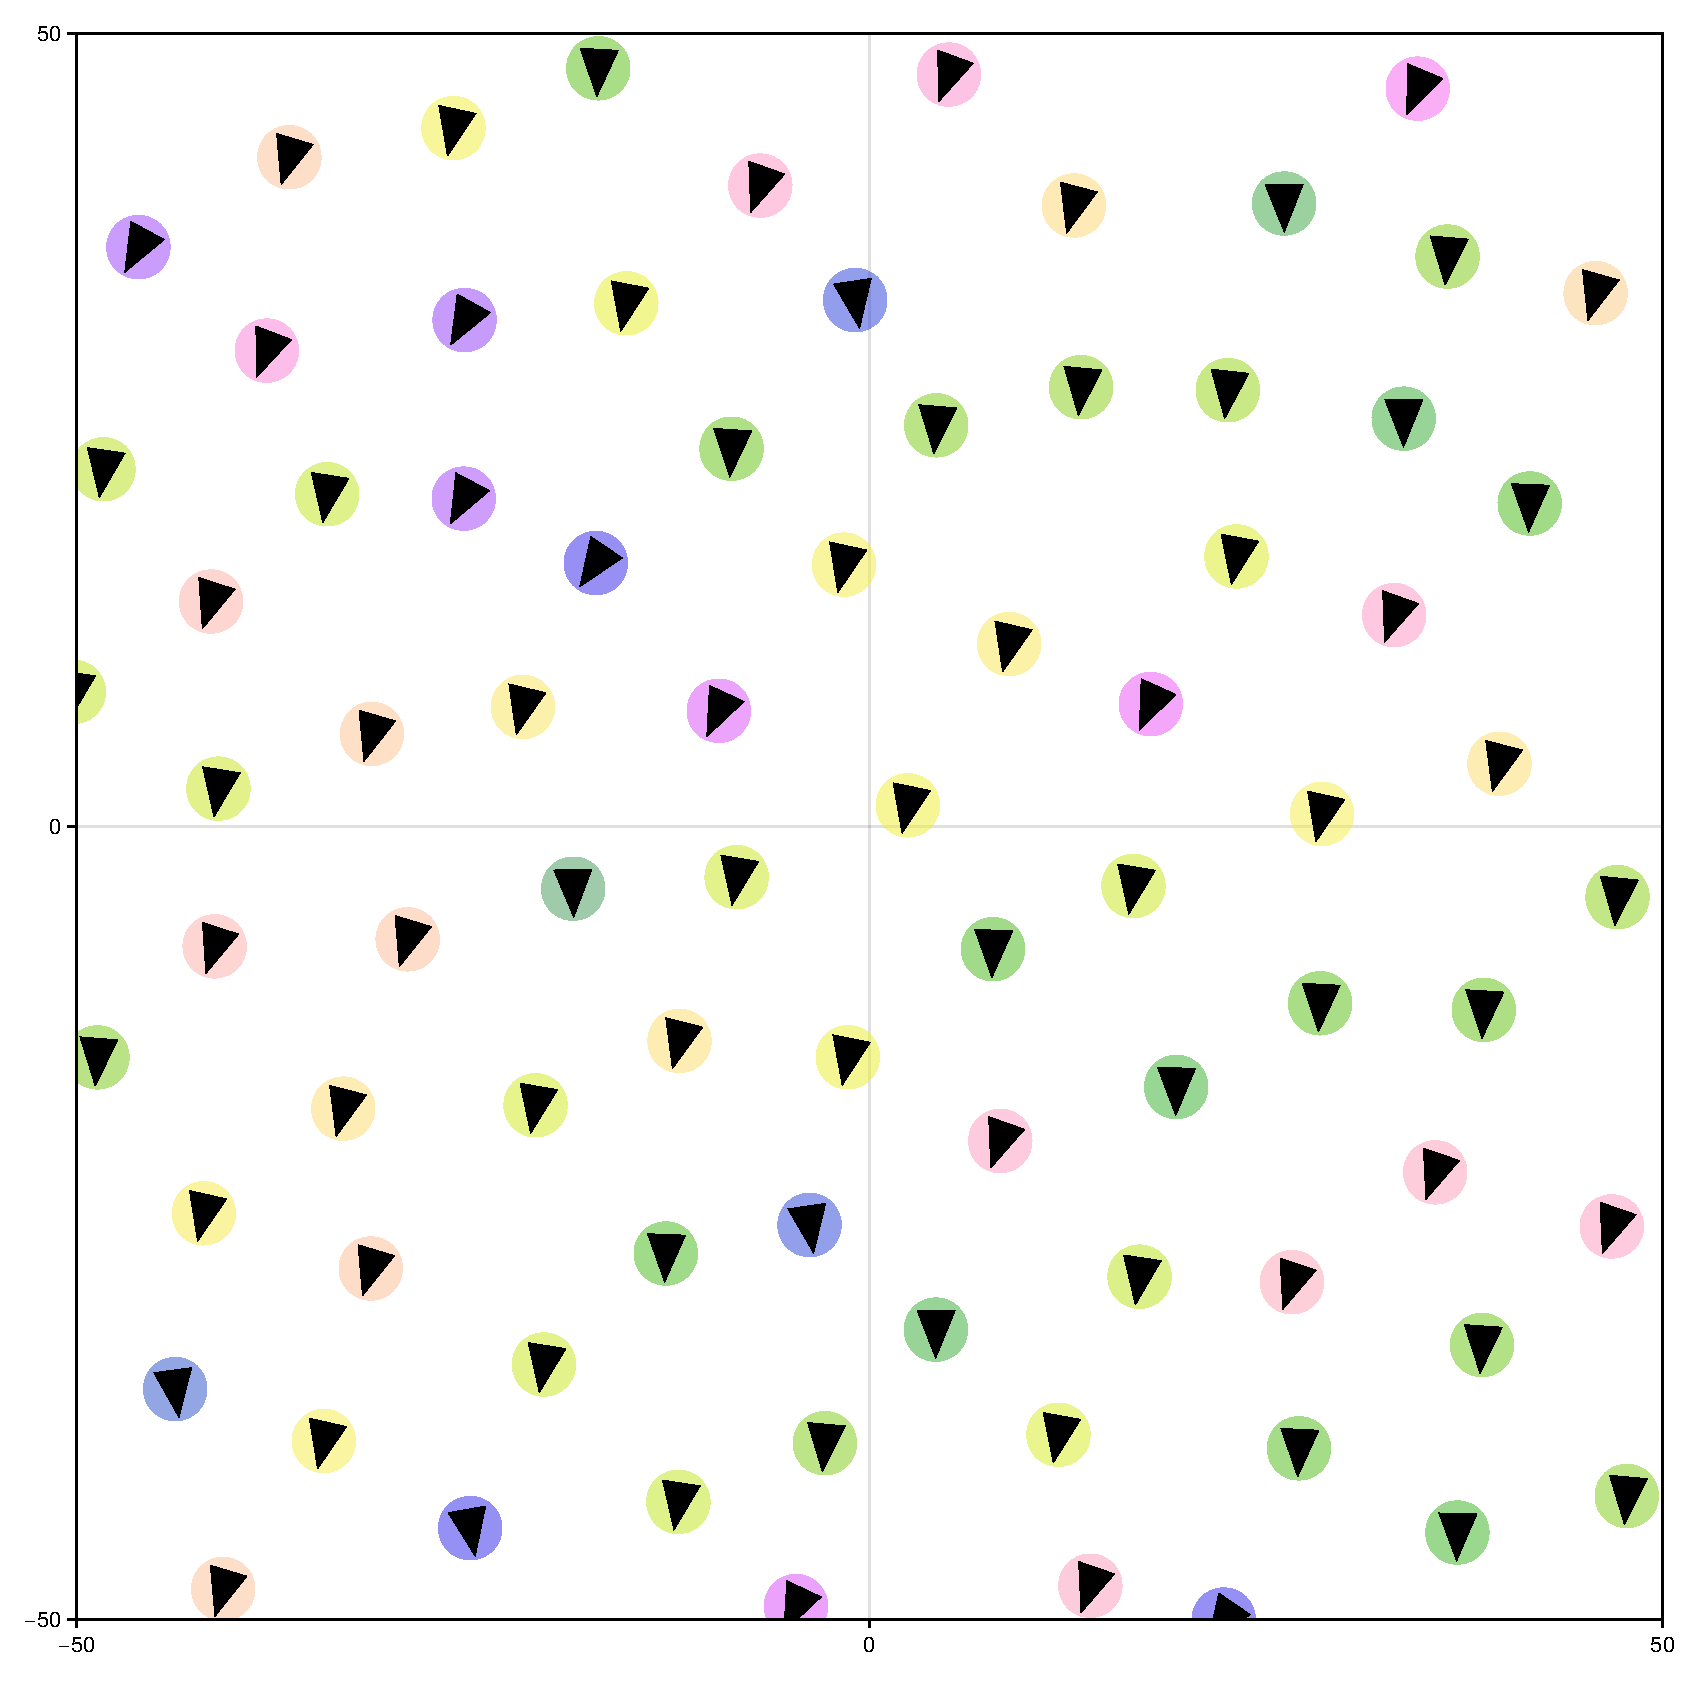
\includegraphics[width=.33\textwidth]{coulombrange40/flocking_20.0s.pdf}}
			\subfloat{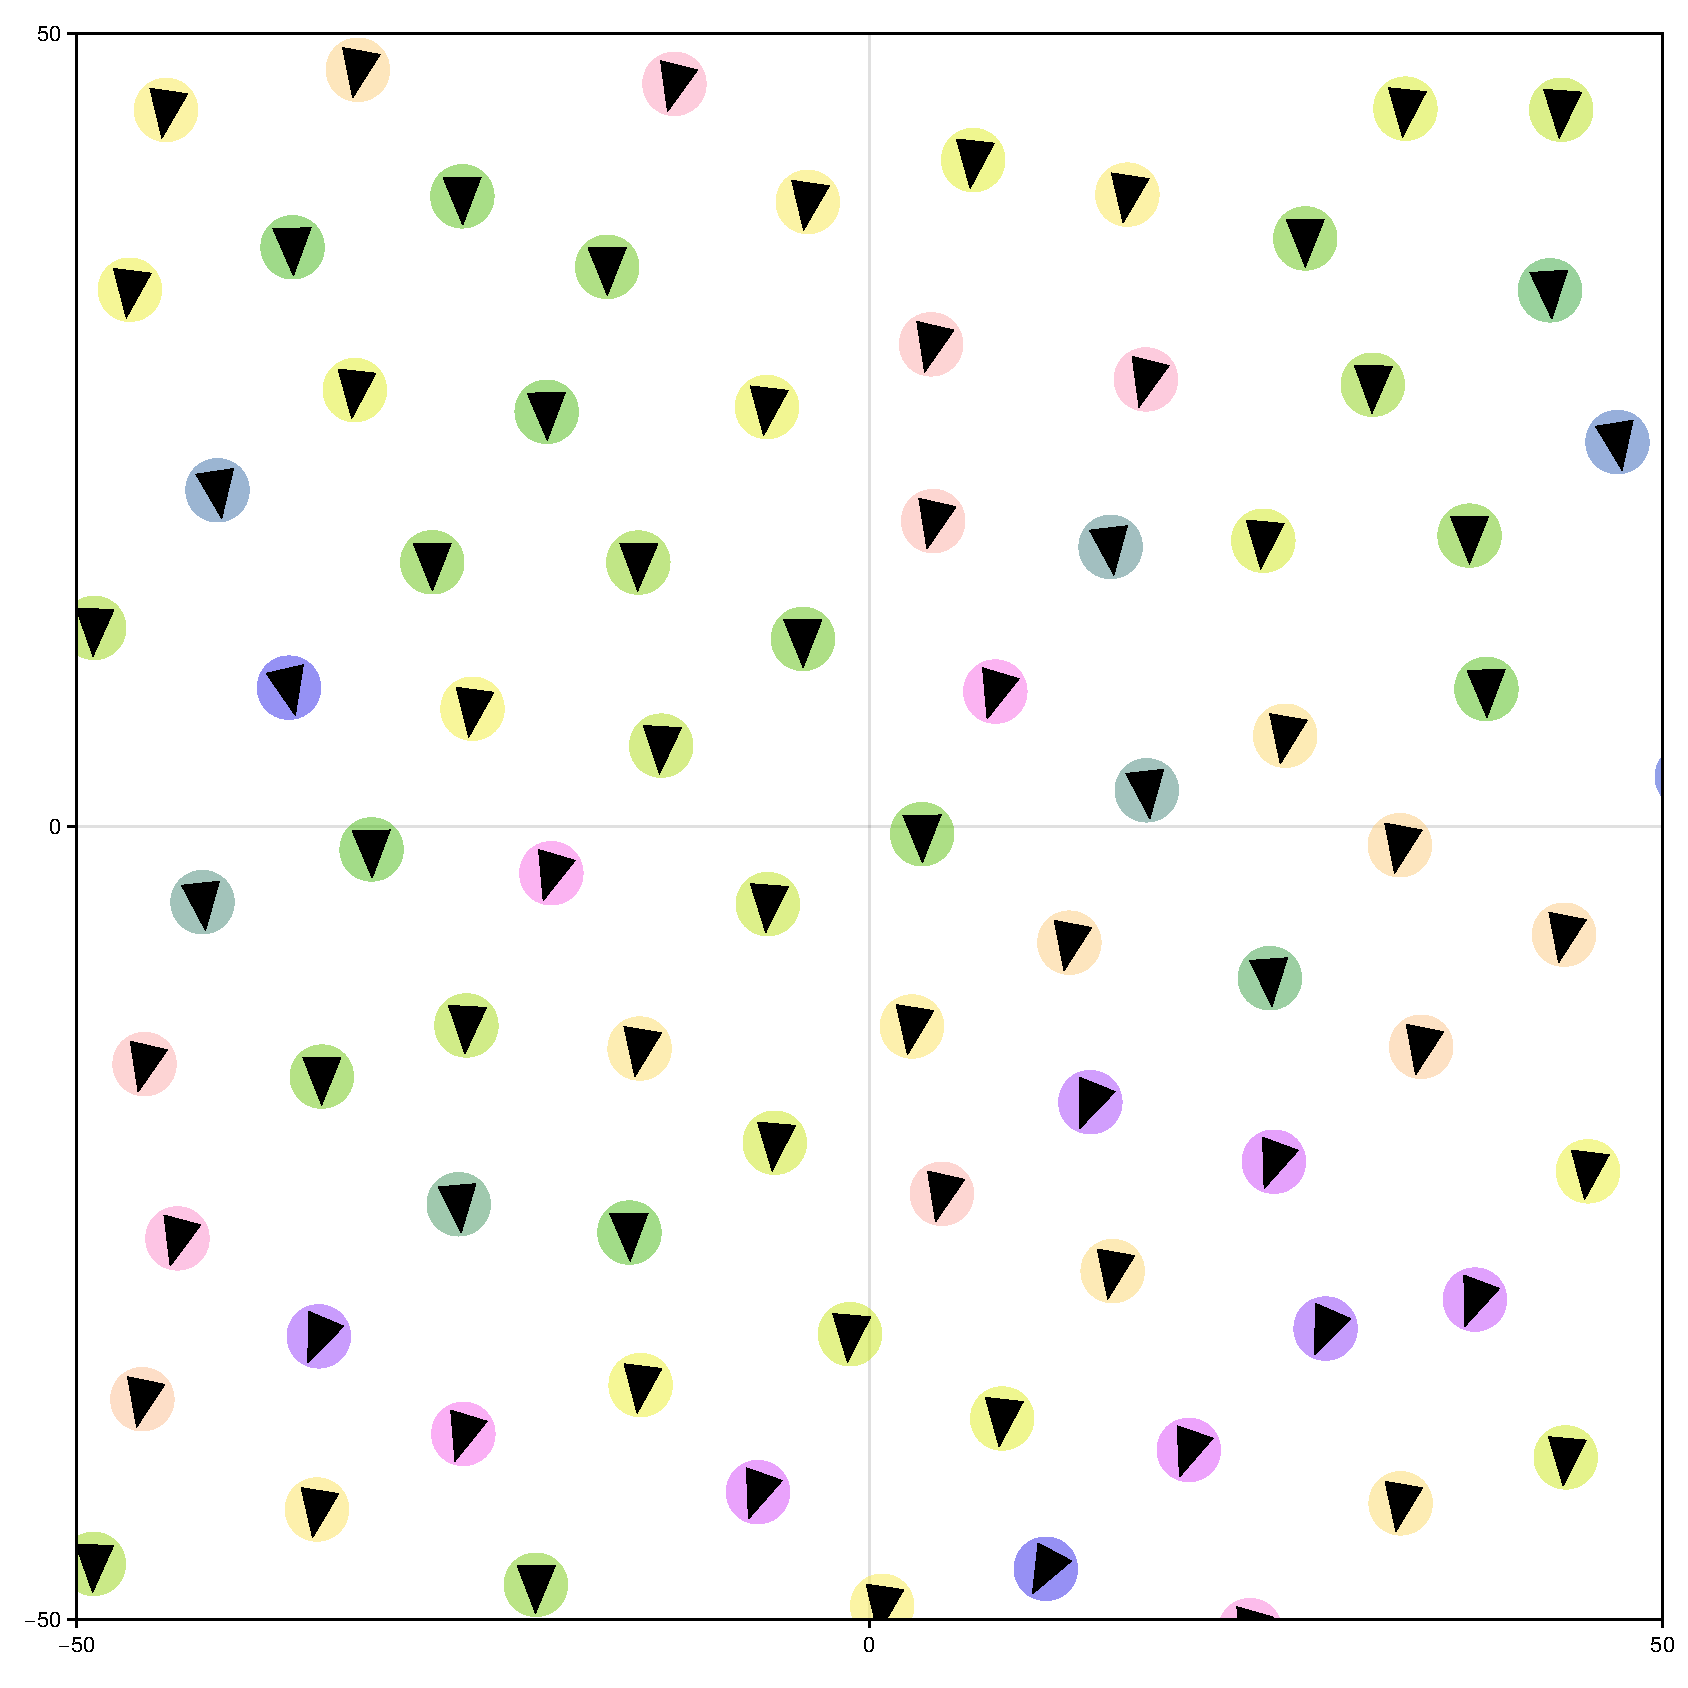
\includegraphics[width=.33\textwidth]{coulombrange40/flocking_25.0s.pdf}}
			\caption{Flocking transition: all particles in the system tend to polarize after few seconds. Images from top left to bottom right correspond to situation after \qtylist{1;5;10;15;20;25}{\second}}
			\label{fig:flock40}
		\end{figure}
		%\todo{ancor meglio se con i secondi direttamenti sulle immagini}
		
		\subsection{Methods}	
		We studied flocking as a II order phase transition, using the global polarization $P$ as order parameter and varying $\alpha$, to change the magnitude of orientations coupling. 
		We have $k = 1.0$ and the range of interaction is \SI{5}{\micro\meter}, which, being $2.5R$, with $R$ particle radius, is enough to make particles interact only with one layer of particles around them, simulating a nearest-neighbor interaction.
		%\todo{quant'è $k$? sarebbe forse utile avere un grafico della forza vs. distanza; inoltre spiega perché hai scelto questi valori fissi per il potenziale e hai variato solo $\alpha$ e la velocità}
		Though interactions range is so short, a long-range order establishes for large enough $\alpha$, making the whole ensemble polarize.
		
		Integration step is \SI{5e-2}{\second} and simulation is \num{2e5} steps long, for a resulting simulation time of \SI{e4}{\second}, enough to let the system thermalize and reach a steady state as shown in Figure \ref{fig:polar_therm}.
		Every \num{100} steps, global polarization is computed and appended to a vector that, from now on, will be called the \emph{polarization history} vector.
		For each parameter set, we performed one simulation only: in this aspect, our analysis differs from the one done by \citeauthor{martin-gomez_collective_2018}, where means and standard deviations are computed over independent realizations.
		We believe that, with fixed simulation time, making one longer simulation is more convenient than more shorter ones, since the system has to thermalize only once, letting us waste less data.
		When everything is done in one simulation, some resampling technique is required to compute an estimate of the error as will be explained shortly.
		We proceeded to analyze data as follows: after discarding the first \num{2e4} steps (\SI{1000}{\second}) as thermalization, the polarization history vector is treated using both a blocking and a JackKnife resampling.
		
		\begin{figure}[hbtp]
			\centering
			\includegraphics[width= \singfigwidth]{phasetrans/thermalization_v10.pdf}
			\caption{Temporal evolution of polarization for $v = \SI{10}{\um\per\second}$, and several values of the off center coupling. Black dashed line is the number of points we discarded.}
			\label{fig:polar_therm}
		\end{figure}
		%\todo{sistema i valori di off-center; mostra polarizzazione tra 0 e 1; metti direttamente i secondi sull'asse delle x; colori difficilmente distinguibili}
		
		Blocking means grouping all the history in subsets of subsequent points and replacing each of them with their average.
		This process is executed in order to compute an estimate of the standard deviation for observables of interest, calculating it as if each block was independent from the others. 
		Choosing the block size is a matter of discussion: a large size will result in blocks with smaller correlation, but the small number of the obtained bins will make oscillations (error on the error) larger. 
		In theory, the value of the standard deviation will saturate to its \emph{real} value increasing the size, but in reality one has to make some trade off with the oscillation size.

		Blocking only will not solve the fact that all data comes from the same sample.
		In order to have good estimators for means and variances of relevant observables we need a resampling technique, such as the well-known Bootstrap or, as we used, JackKnife, where we replace each point with the mean of all the other points in the history.
		Resulting sample standard deviations for polarization and susceptivity are plotted in Figure \ref{fig:blocksize} as a function of block size.
		%\todo{non hai introdotto la suscettività, spiega cosa è e perché la calcoli nella sezione dove descrivi la polarizzazione}
		
		For increasing block size, standard deviation of relevant observables approaches its limit value, while oscillations around this value increase as the number of blocks becomes smaller.
		We used \num{2500} as a block size, to saturate the standard deviation while containing the amplitude of oscillations, as is explained in \ref{fig:blocksize}.
		
		\begin{figure}[hbtp]
			\centering
			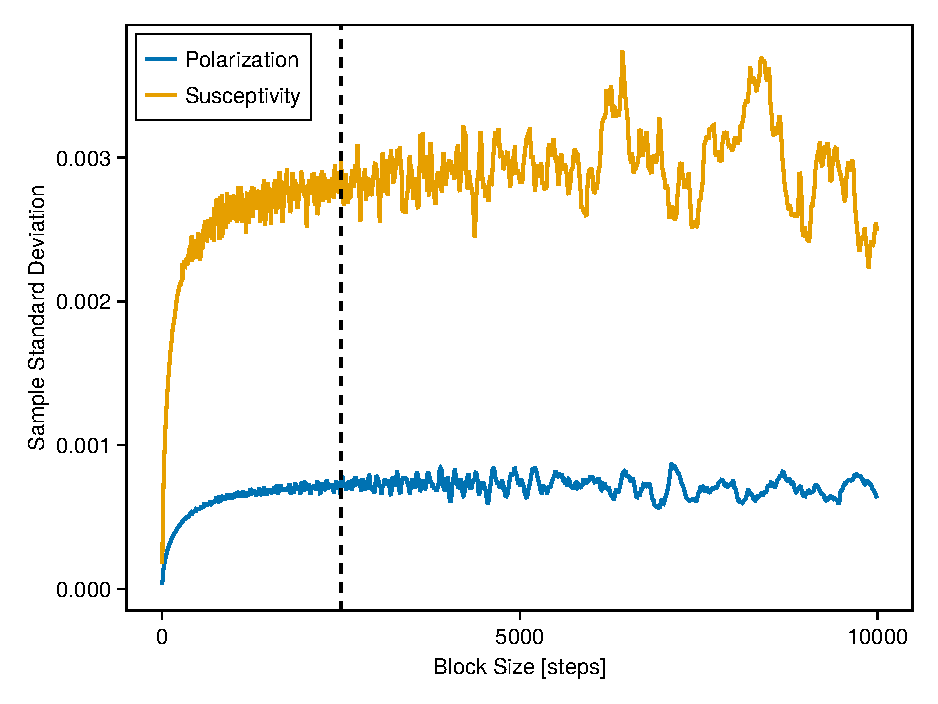
\includegraphics[width= \singfigwidth]{phasetrans/blocksize_v10.pdf}
			\caption{Standard deviation of polarization and susceptivity versus blocking size. Black dashed line is the block size of 2500 points that was used for this work. For this plot, $v = \SI{10}{\um\per\second}$, $\alpha = 0.25$. Both a blocking procedure and a JackKnife resampling are used here.}.
			\label{fig:blocksize}
		\end{figure}
		%\todo{non ho capito, hai usato il blocking o il jackknife?}
		
		Using both the blocking and JackKnife resampling, we compute standard deviations taking care of auto-correlations in data.
		
		
		\subsection{Results}
		
		For every value of $\alpha$, polarization is taken as the mean of the polarization history vector, with thermalization cut off, while we computed susceptivity using both a blocking and a JackKnife resampling.
		As a result, Figure \ref{fig:phasetrans} shows the expected behavior of a II order phase transition: as polarization $P$ jumps with a discontinuity from 0 to 1, its susceptivity has a peak when $\alpha$ approaches critical value and then returns back to zero (see, as a reference, Figure \ref{fig:martin_flocking3}).
		Here we notice how the susceptivity peak shifts up and to the right for decreasing velocity.
		
		Though the lowest-energy configuration is the one with all particles aligned due to the repulsion that take place between the fronts of interacting particles, this model does not present an explicitly aligning torque like the one of the form $T \sim \sin( \theta_{i}-\theta_{j} )$ used by \citeauthor{martin-gomez_collective_2018}.
		Still, a flocking phase transition takes place with an evolution akin to the one showed in \cite{martin-gomez_collective_2018} as graphs in Figure \ref{fig:phasetrans} clearly show.
		Here, the off-center parameter $\alpha$ plays the role of the coupling $g$ in reference paper.
		In cited work, Péclet number was changed to see its effect, while here we used velocity as an equivalent parameter, with the only disadvantage of not being non-dimensional. 
		
		%\todo{presenta e discuti i risultati in maniera più dettagliata; non si capisce quale tecnica di resampling hai usato; spiega meglio cosa rappresentano i grafici e come sono stati ottenuti}
		
		\begin{figure}[htp]
			\centering
			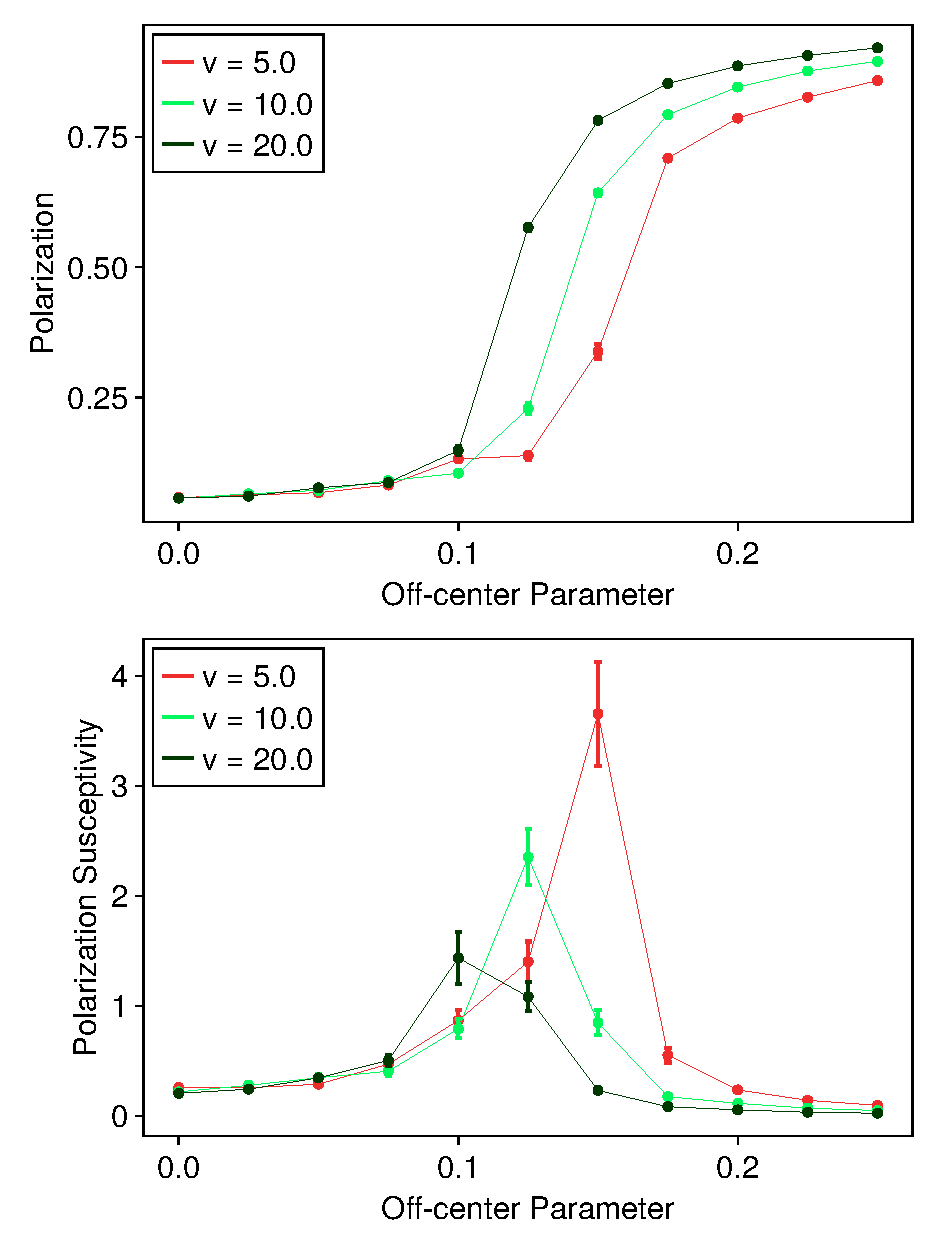
\includegraphics[width= \singfigwidth]{phasetrans/pol_susc.pdf}
			\caption{Diagrams for polarization and relative susceptivity for the transition to ordered phase.}
			\label{fig:phasetrans}
		\end{figure}
		%\todo{perché lo stile di questta figura è così diverso da quello delle altre? mancano le unità di misura delle velocità}
		
		\section{Clustering and Local Order}
		Lennard Jones (LJ) is a standard potential in interacting ABPs analysis and it has a chance of representing well real world dynamics (see section \ref{qualitative}), thus making it important to study its effects on ABPs collective dynamics. 
		To quantify this effect in various situations, we investigated both global and local polarization, as well as clustering, to better understand the effects of the different model parameters on both positional and orientational degrees of freedom.
		As discussed in section \ref{qualitative}, in experiments not all particles move with the same self-propulsion velocity because of imperfections in fabrication processes.
		For the same reason, some particles show a nonzero angular velocity that makes their dynamics more well-explained by a Chiral Brownian motion \cite{callegari_numerical_2019}.
		Thus, to capture these experimental observations, we added aforementioned features in simulations, and then studied how such features can change collective behaviors of an ensemble of self-propelled particles.
		
		From now, unless otherwise stated, the interaction used is Lennard Jones with parameters $\sigma = 2R$, and strength parameter $\epsilon  = \SI{0.1}{\pico\joule}$.
		The value for $\sigma$ is kept fixed to respect the natural units of the system, while the strength parameter is enough to make the system cluster with the right parameters while keeping the integration step not too low.
		Interaction range here is \SI{40}{\um}, or $10\sigma$; we chose this value not for physical reasons but for speed sake: because it is the cutoff distance after which LJ force magnitude becomes smaller than $10^{-6}\abs{F_{min}}$, where $F_{min}$ is the minimum value of the force, computing forces smaller than that will be completely irrelevant for our purpose and just make simulations heavy.
		Simulations involved $250$ particles with $R = \SI{2}{\um}$ in a square of \SI{175}{\um} side, for a resulting packing fraction of $\sim 0.1$.
		Simulation time is 1000 s but shorter times are showed in graphs as needed.
		Integration step can vary with parameters, to ensure the best trade-off between stability in the simulations and execution speed, but for most simulations \SI{5e-3}{\second} was chosen as integration interval and when different values are used they are declared in sections.
		
		For every parameters set, we simulated five randomly generated starting conditions.
		When distributions are involved in the simulation, e.g.\ for linear and angular velocity, probability distribution functions are resampled at every repetition.
		For cluster size and number, as well as polarization figures, lines in graphs are averages of those five simulations, with ribbons around them represent standard deviations around the mean.
		Radial distribution functions are plotted for the final instant of just one of the simulations.
		Transient time for polarization is measured as the time it takes for this order parameter to reach \num{95} \% of its maximum.
		
		\subsection{Velocity}
		\label{velocity}
		In order to study the effect of velocity, we first computed all the quantities of interest in the case of passive particles with an aligning LJ interaction, and then added a self propulsion velocity. 
		This active velocity results in non-isotropic system, giving a preferred, giving a preferred direction to particles, so we also investigated how velocity interacts with the sign of the directional coupling parameter $\alpha$, repeating the analysis for positive and negative values.
		
		\begin{figure}[hbtp]
			\centering\
			\subfloat[][]{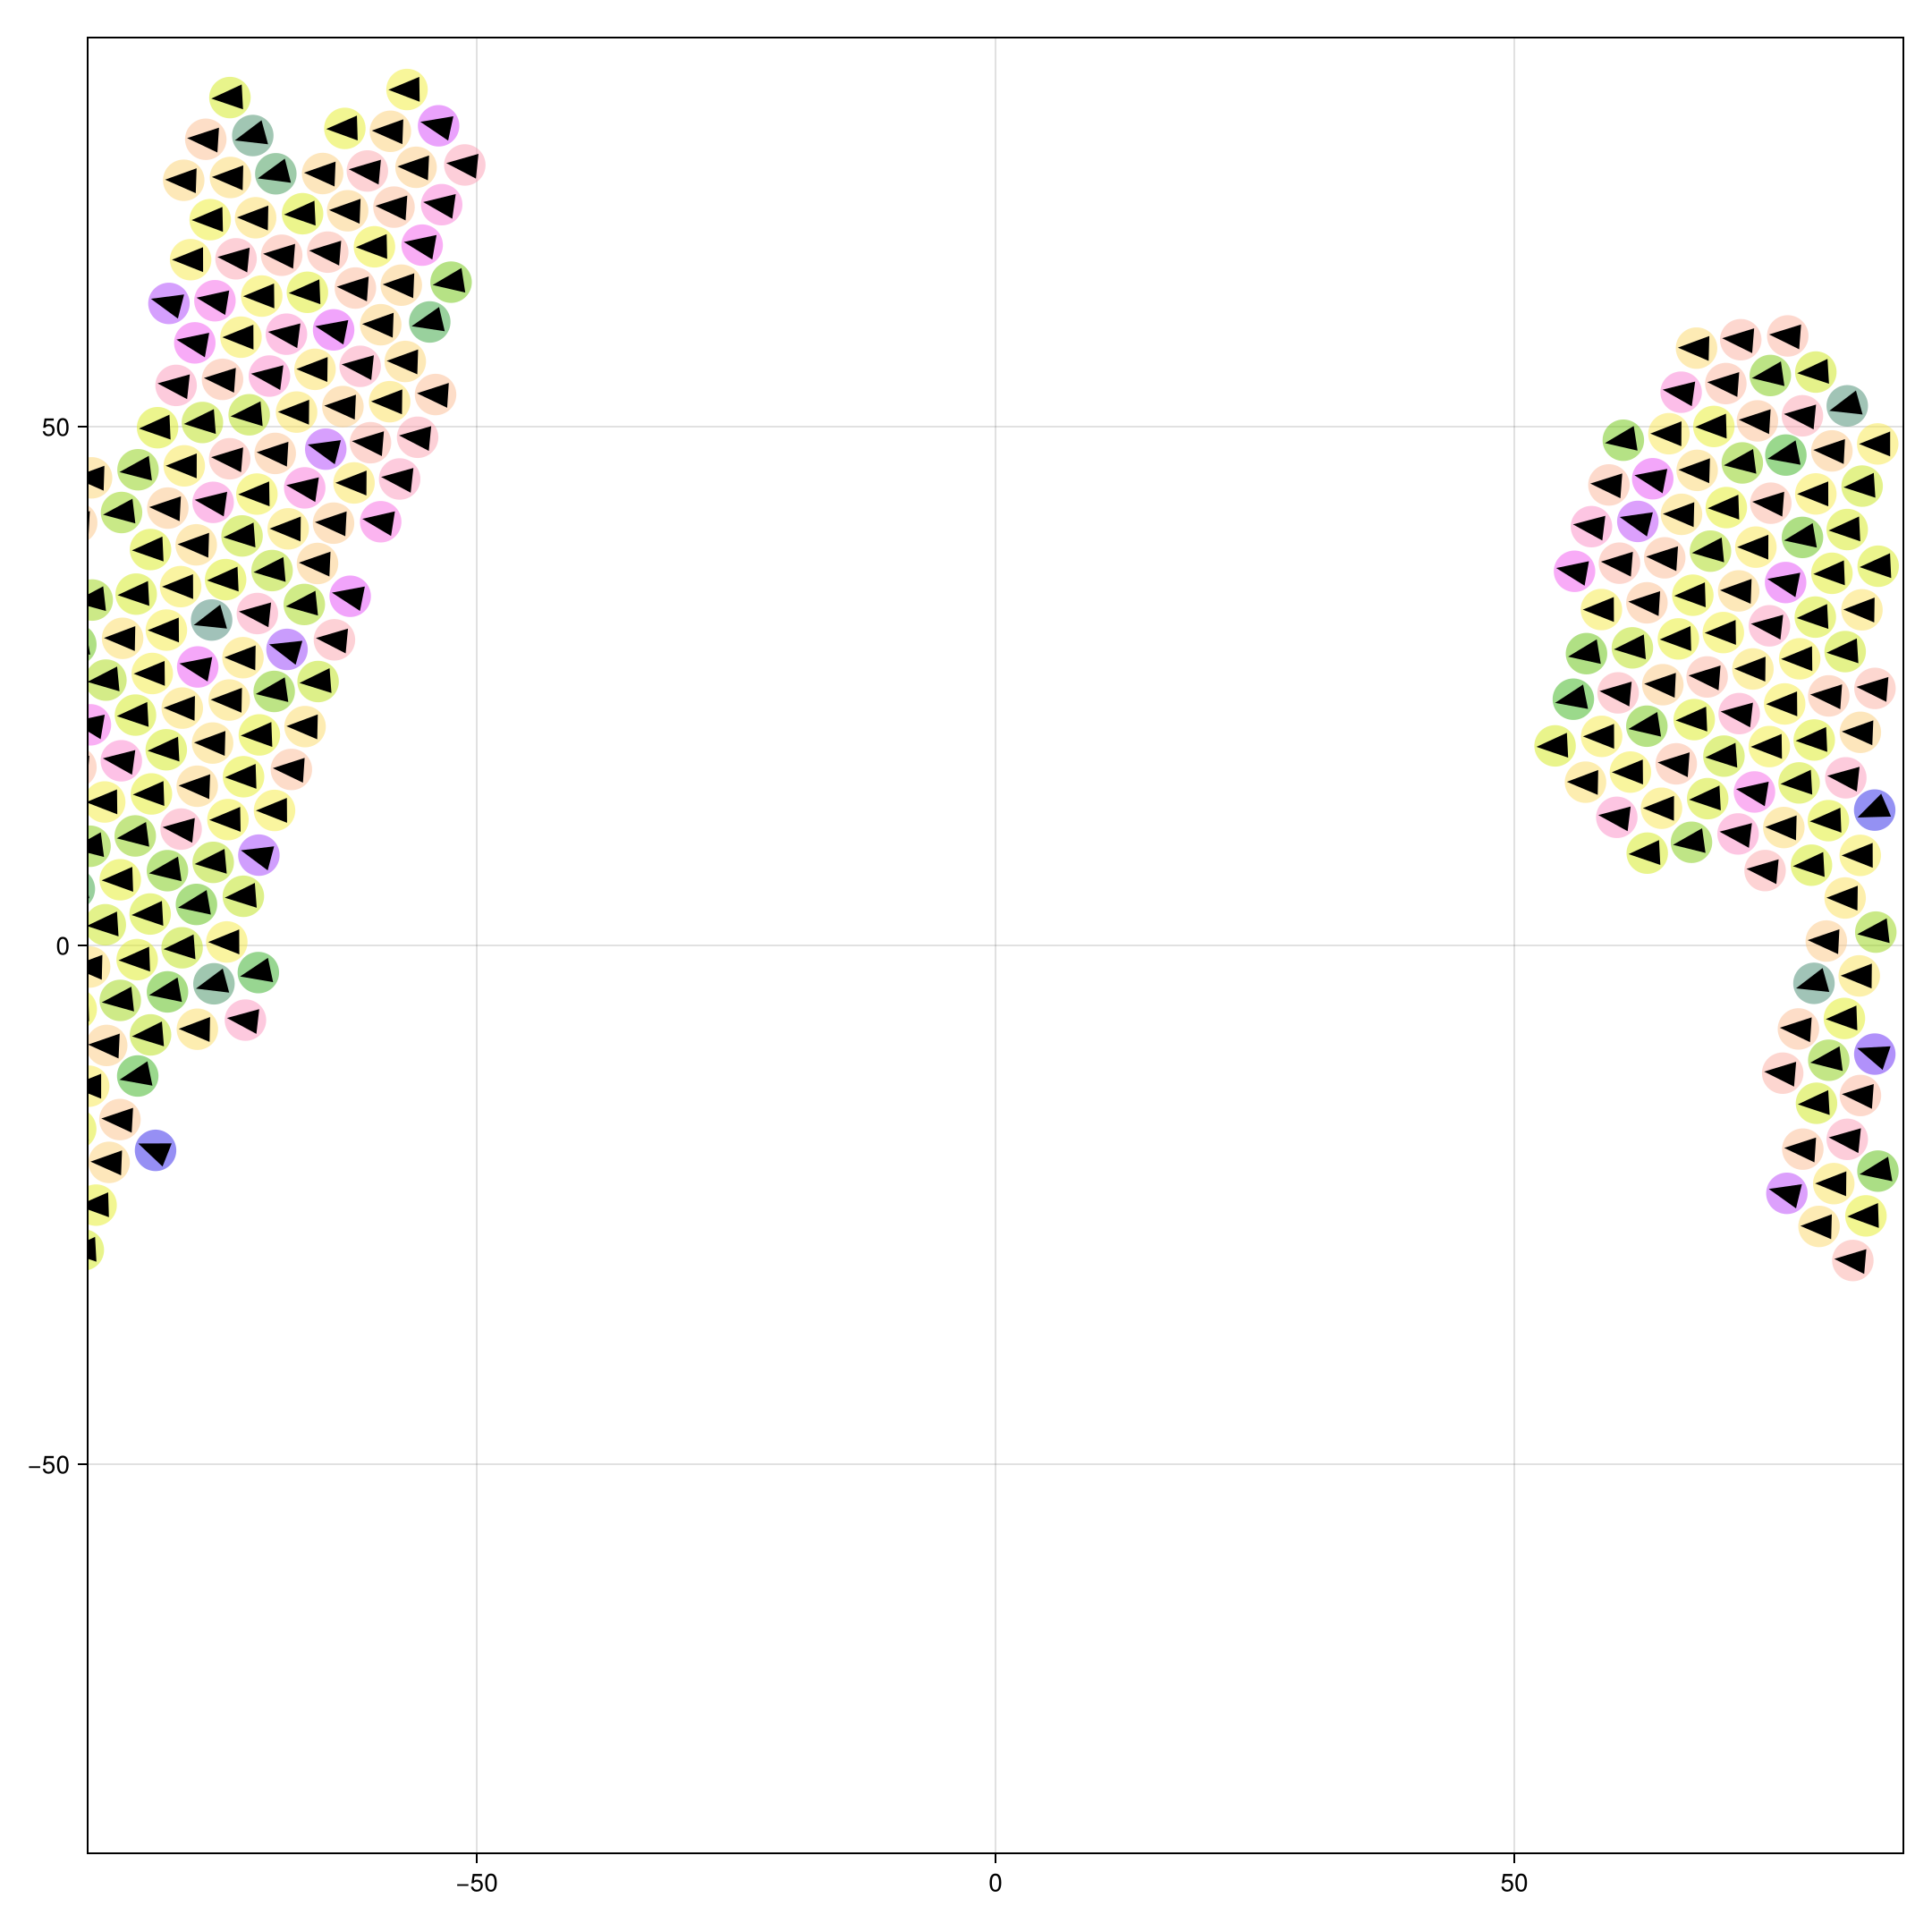
\includegraphics[width=.5\textwidth]{lj_velocity/situa10.0_oc0.5.png}}
			\subfloat[][]{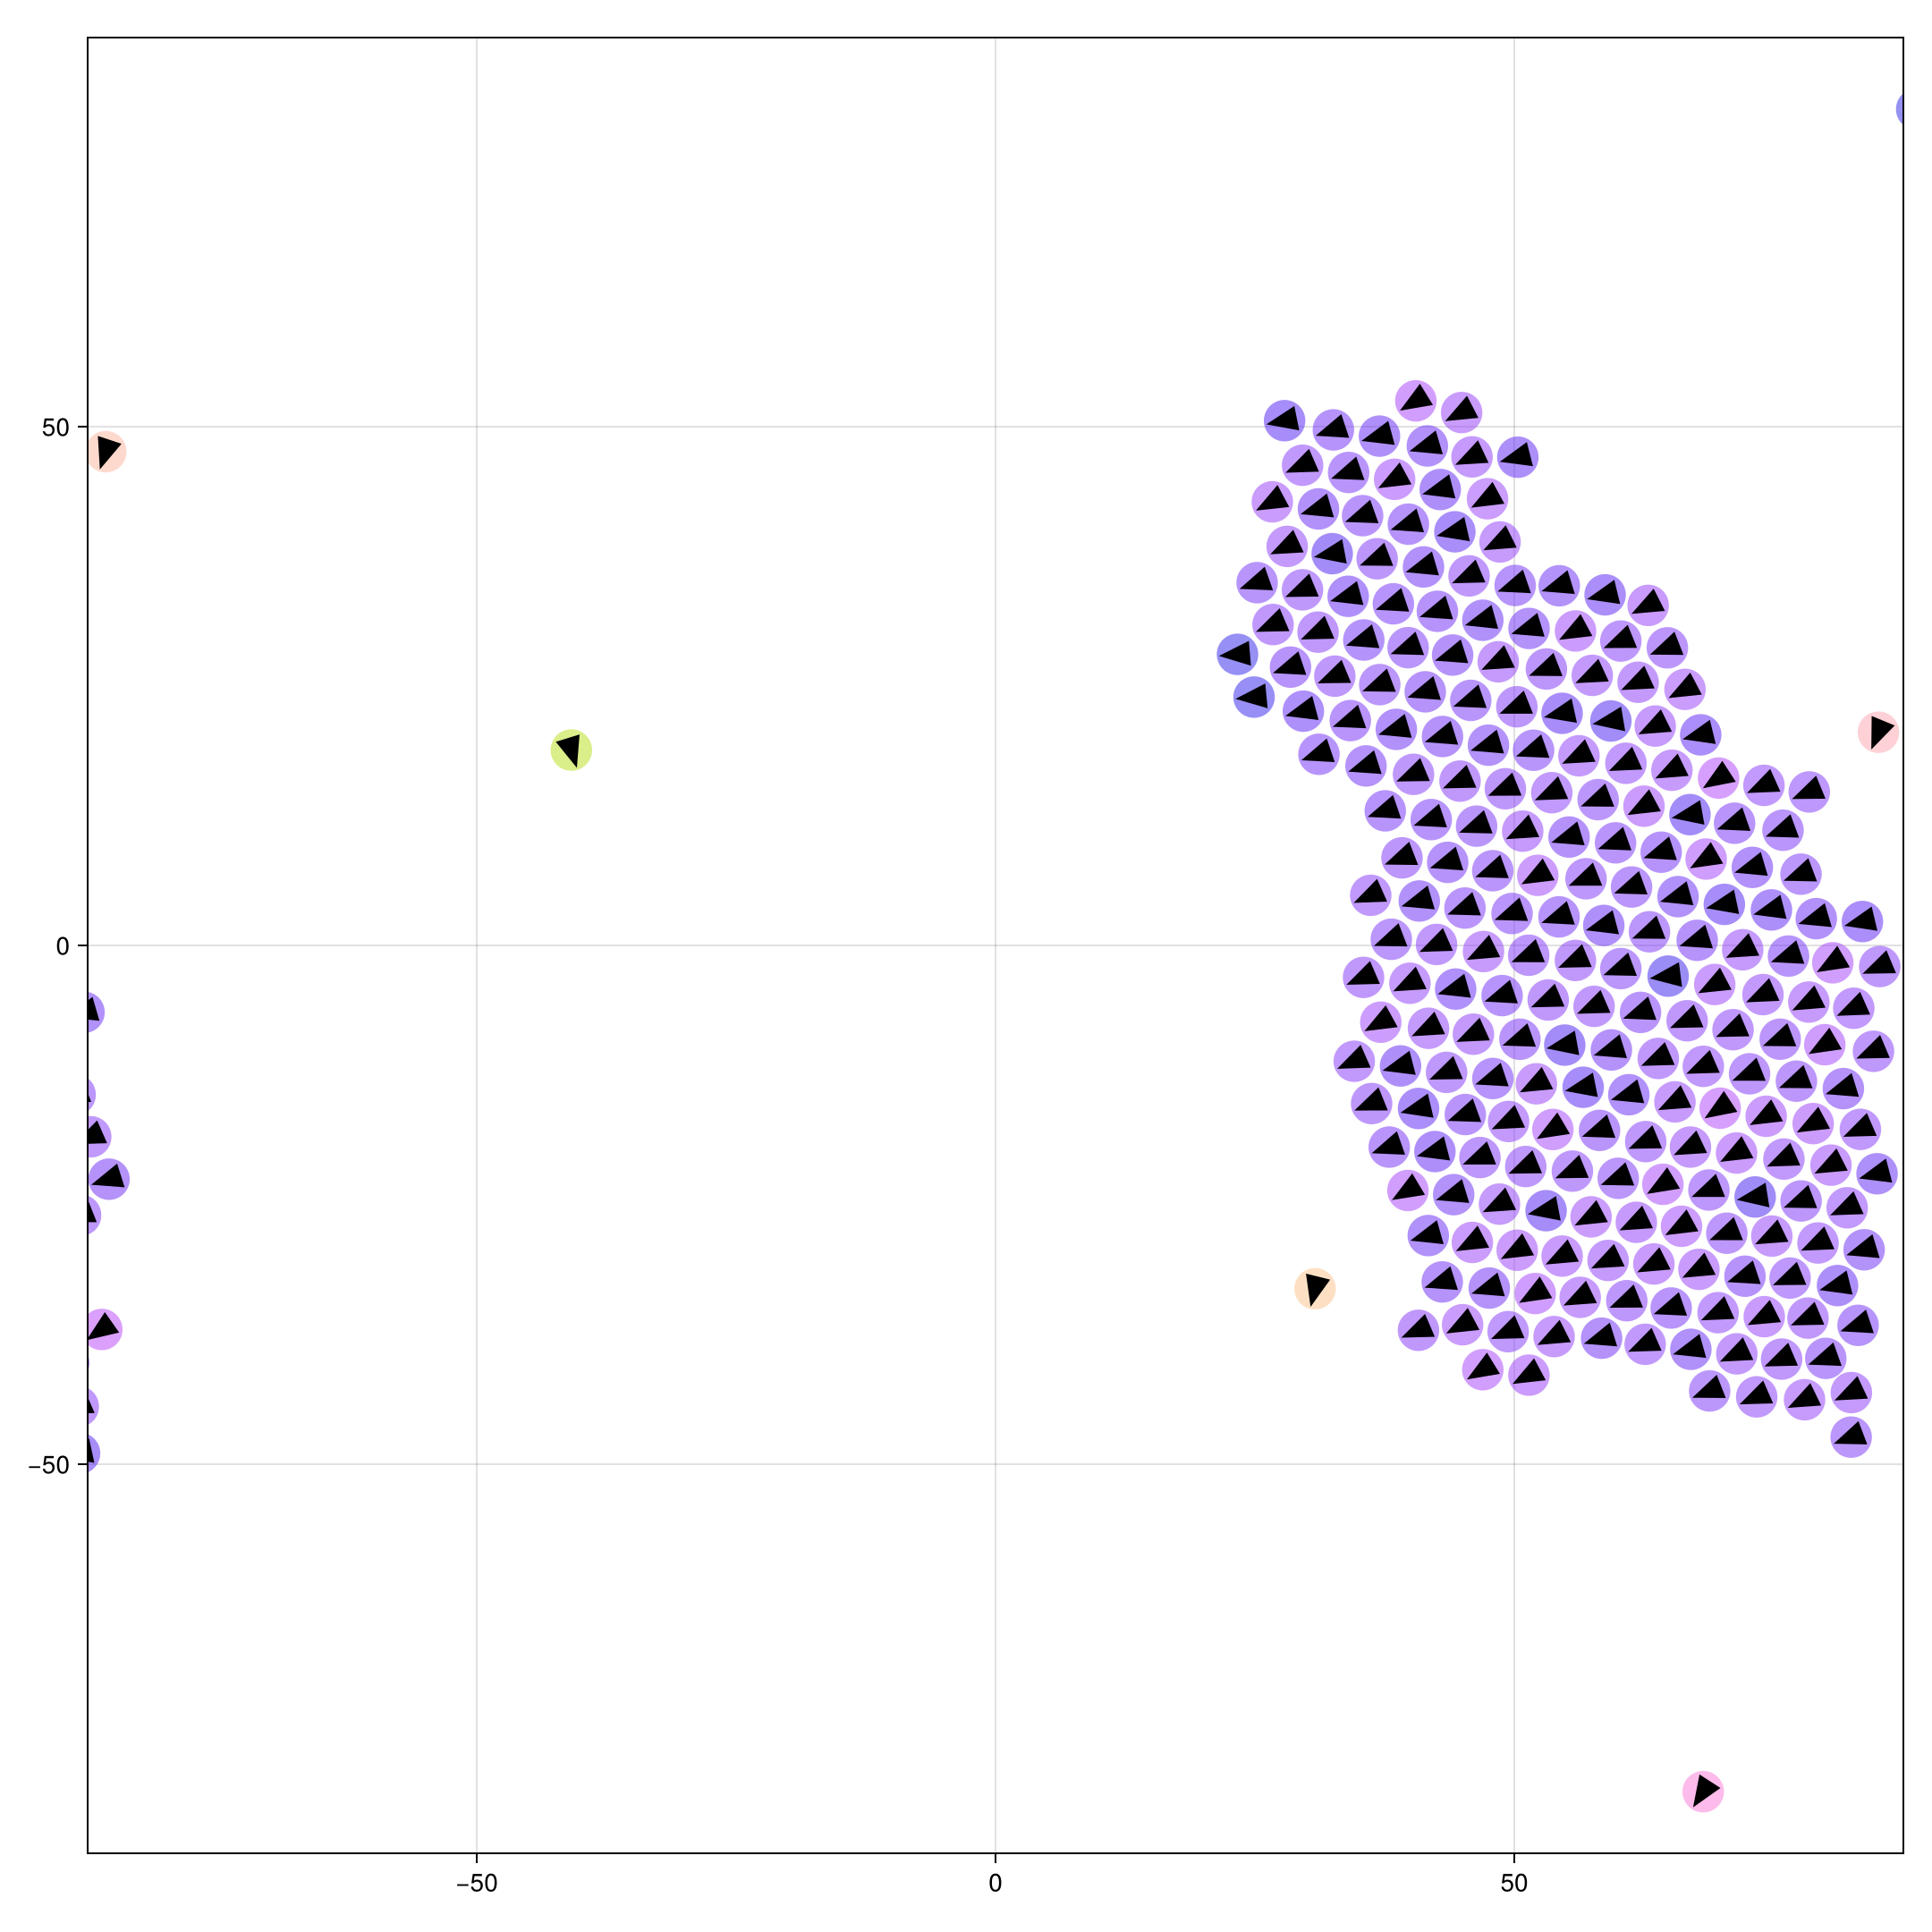
\includegraphics[width=.5\textwidth]{lj_velocity/situa20.0_oc0.5.png}}\\
			\subfloat[][]{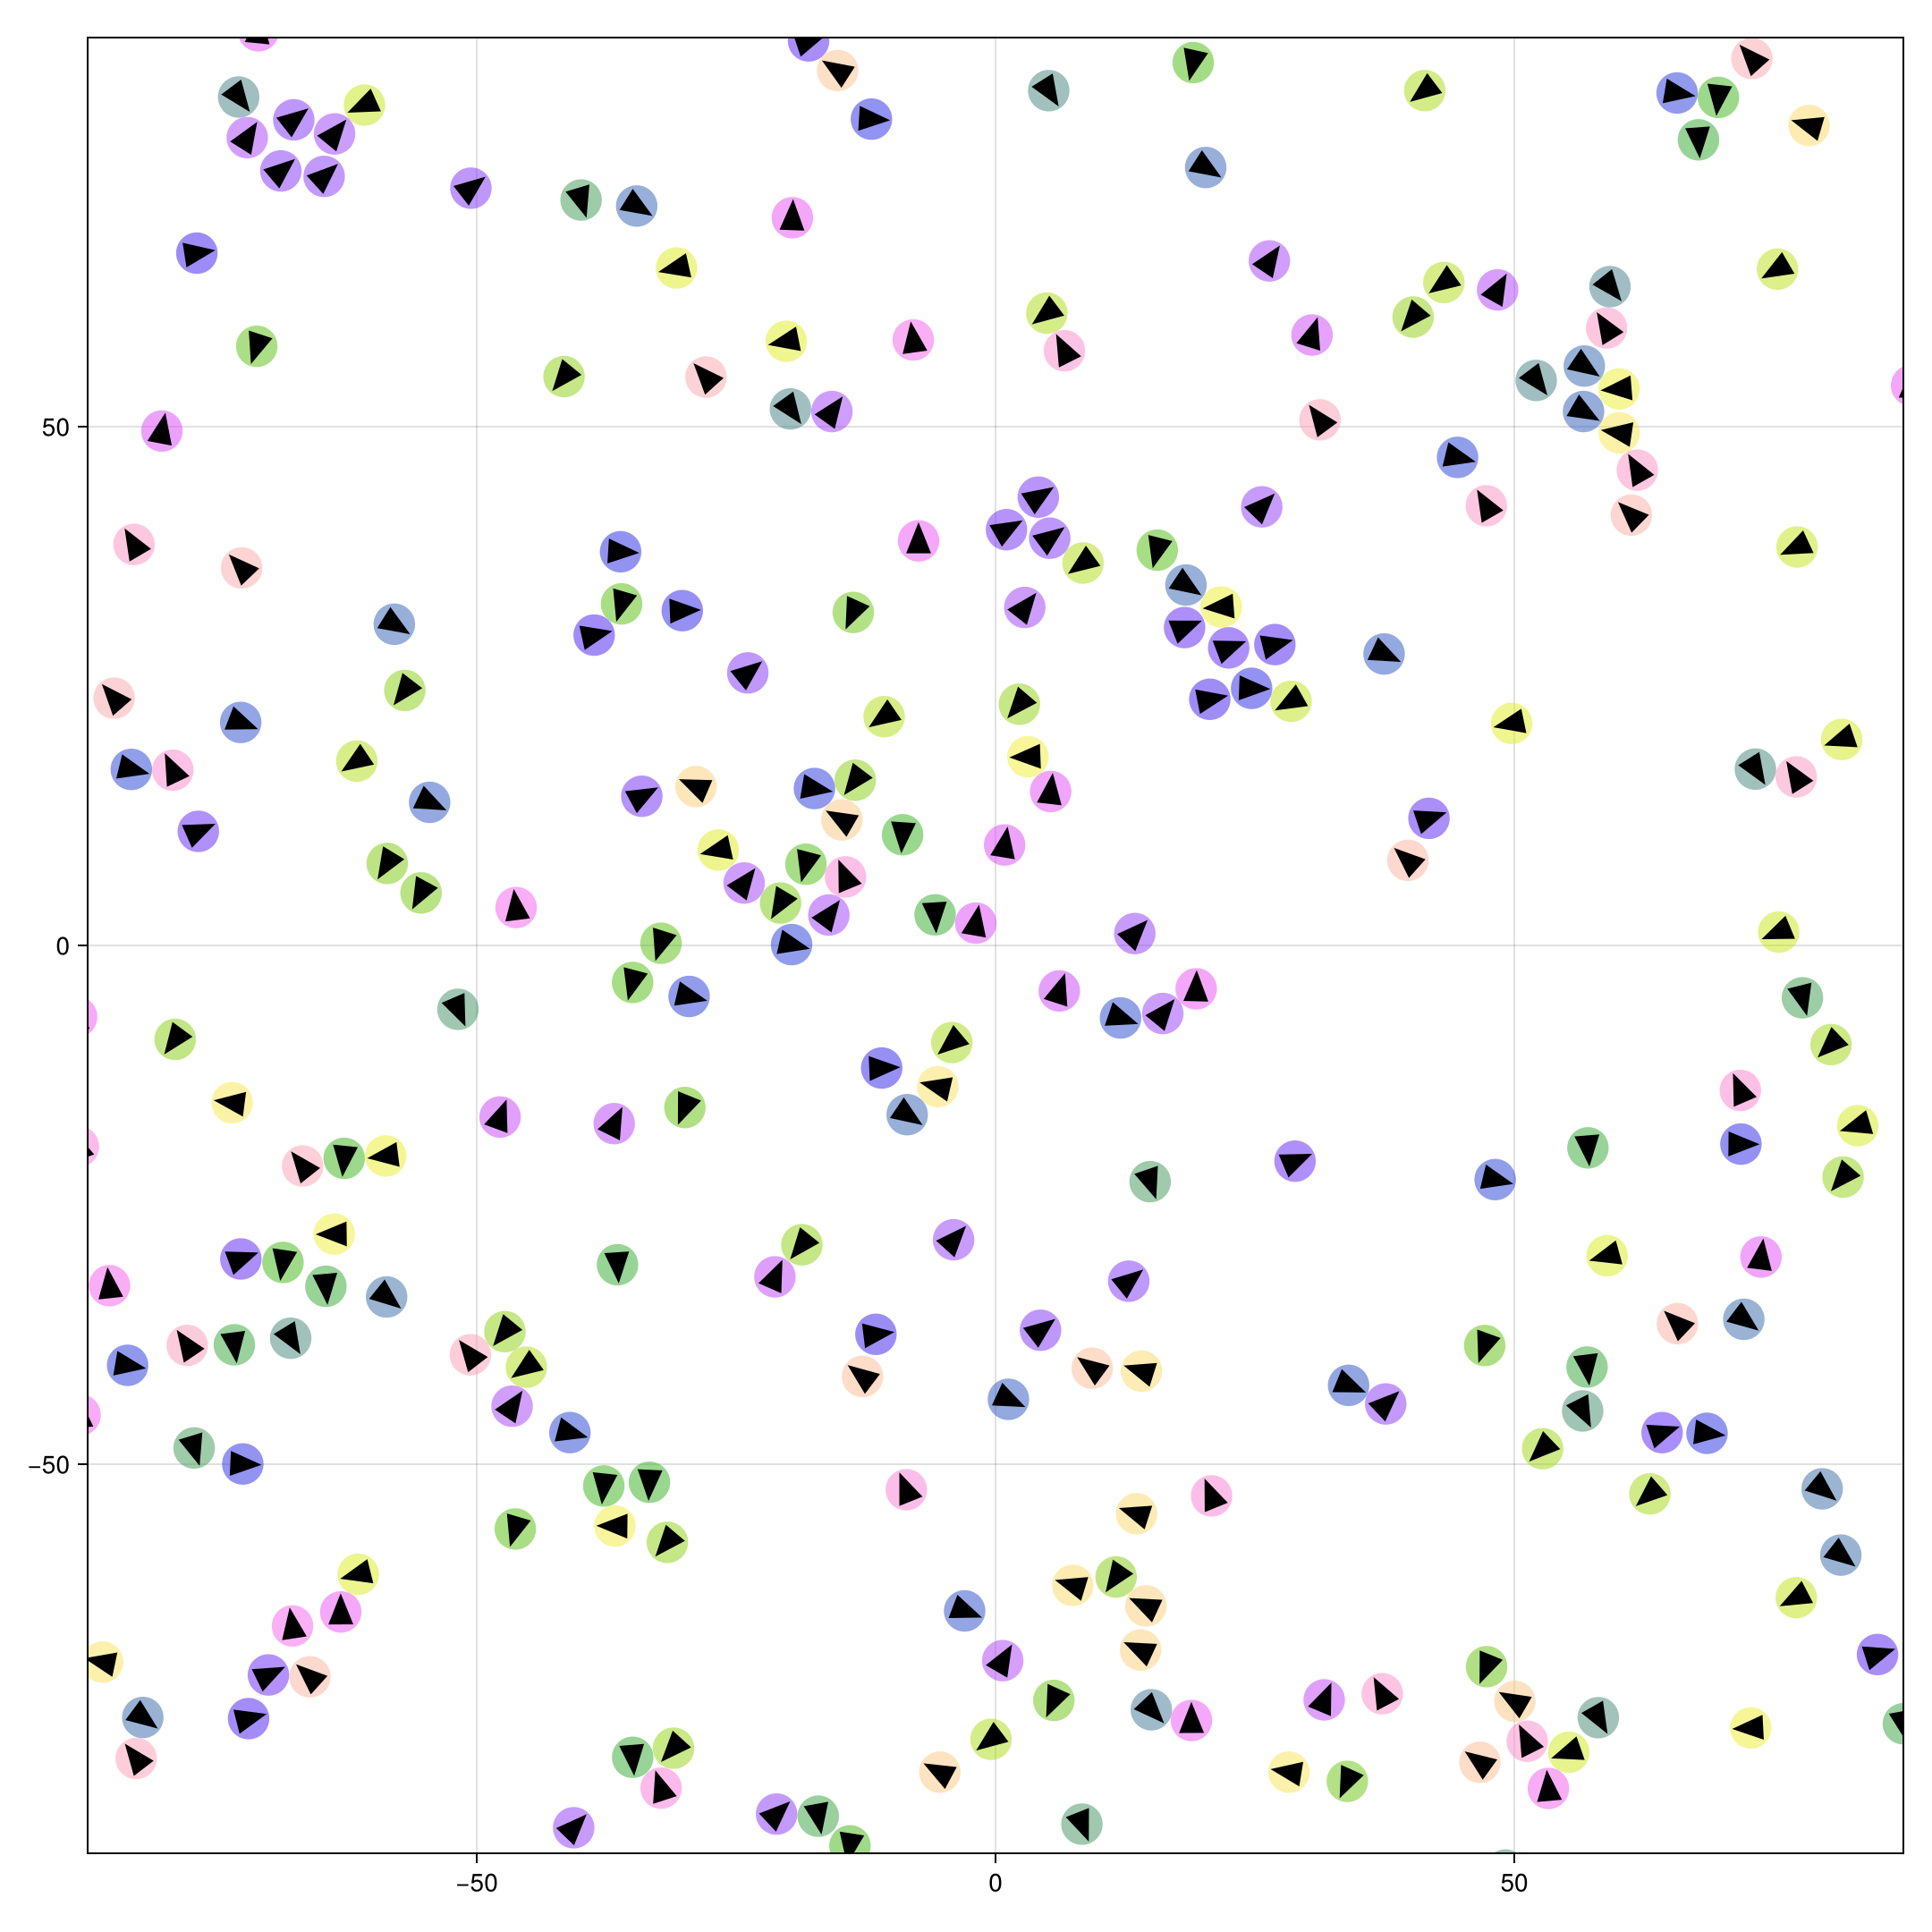
\includegraphics[width=.5\textwidth]{lj_velocity/situa10.0_oc-0.5.png}}
			\subfloat[][]{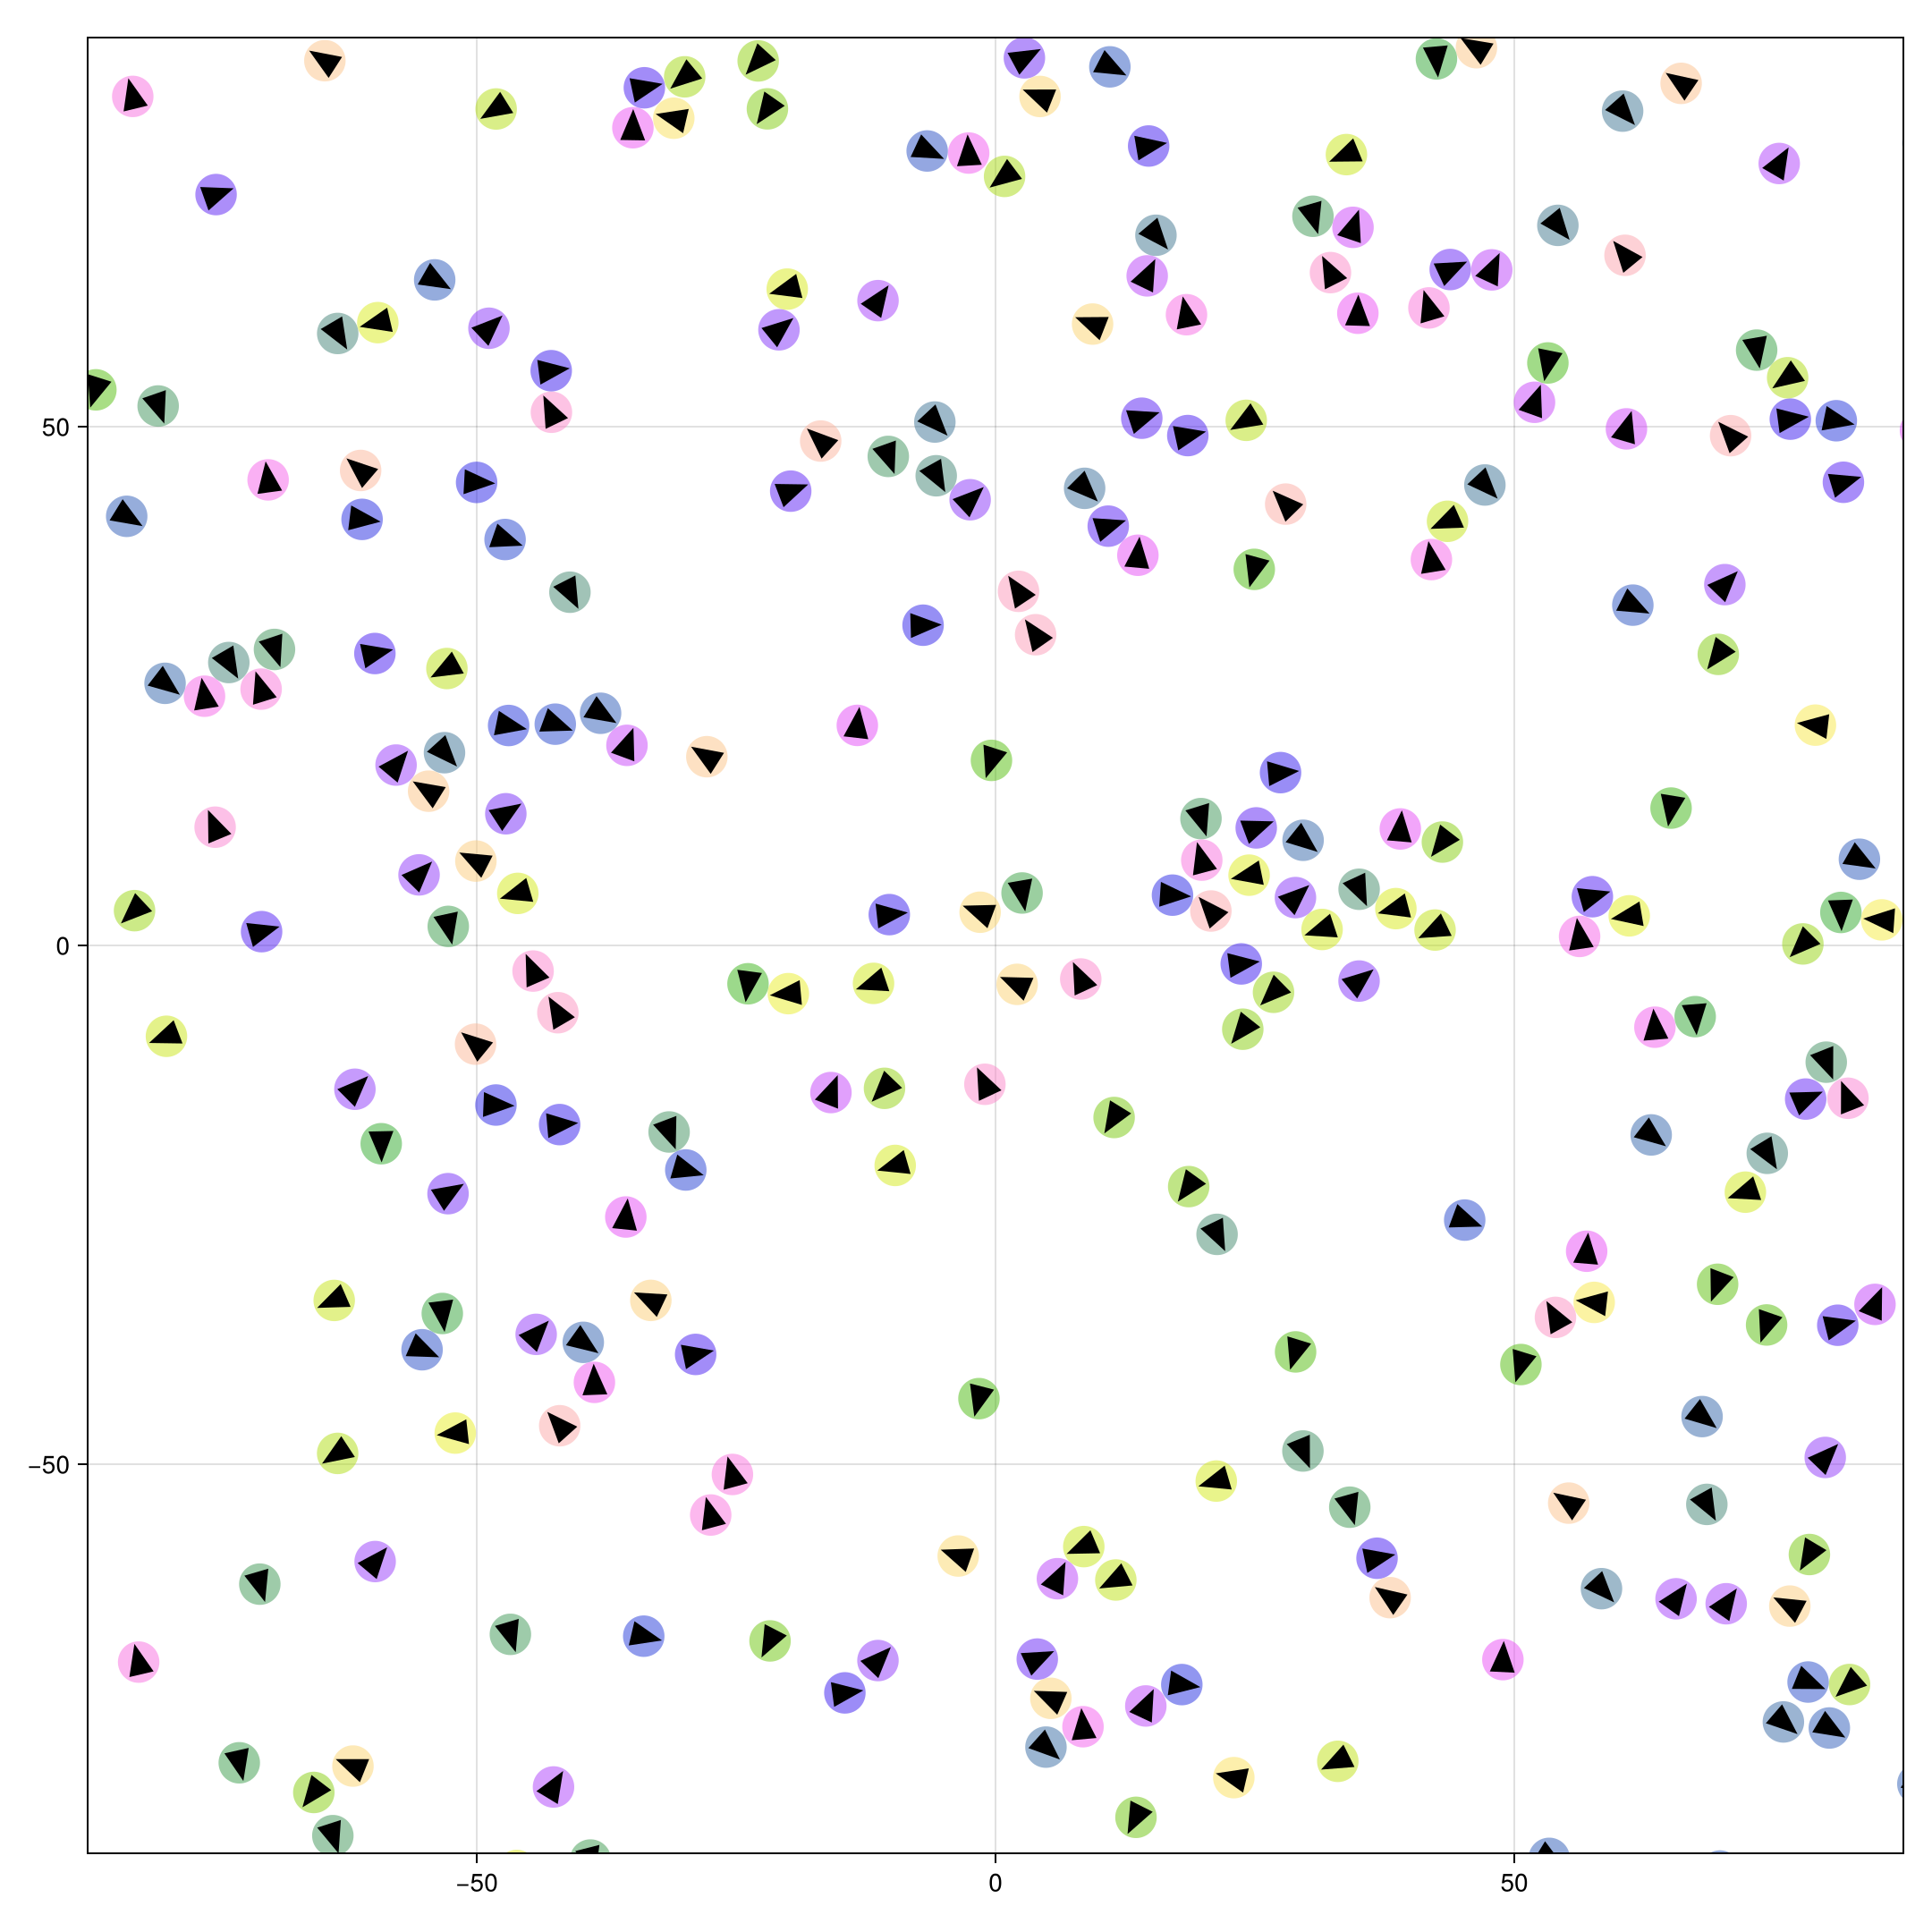
\includegraphics[width=.5\textwidth]{lj_velocity/situa20.0_oc-0.5.png}}\\
			
			\caption{Representative simulation snapshots corresponding to values of velocity and $\alpha$: (a) $v = \SI{10}{\um \per \second} \alpha = 0.5$, (b) $v = \SI{20}{\um \per \second} \alpha = 0.5$, (c) $v = \SI{10}{\um \per \second} \alpha = -0.5$, (d) $v = \SI{20}{\um \per \second} \alpha = -0.5$}
			\label{fig:lj_velocity_situa}
		\end{figure}
		
		In Figure \ref{fig:lj_velocity_pol} it is noticeable how an ensemble of passive particles with an aligning interaction has a baseline local polarization, while the global is almost zero. 
		Adding self-propulsion has the consequence of making the system polarize, with a transient duration that depends on the velocity: faster particles tend to align faster. 
		A noteworthy characteristic is that particles with interacting position on the back do not tend to align globally, and local polarization does not rise over the baseline value.
		
		\begin{figure}[hbtp]
			\centering\
			\subfloat[][]{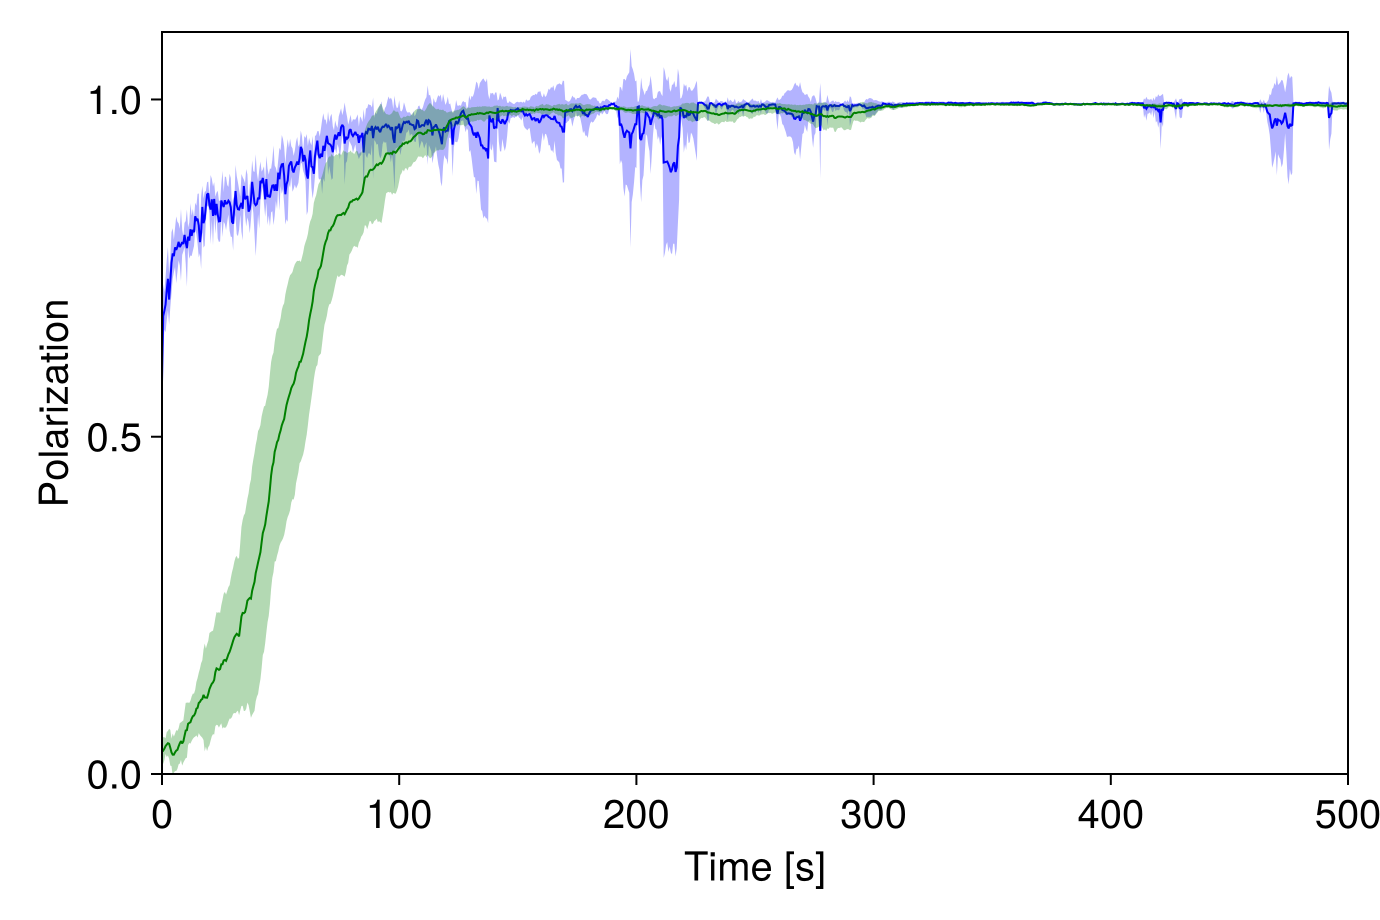
\includegraphics[width=.9\textwidth]{lj_velocity/polar10.0_oc0.5.png}}\\
			\subfloat[][]{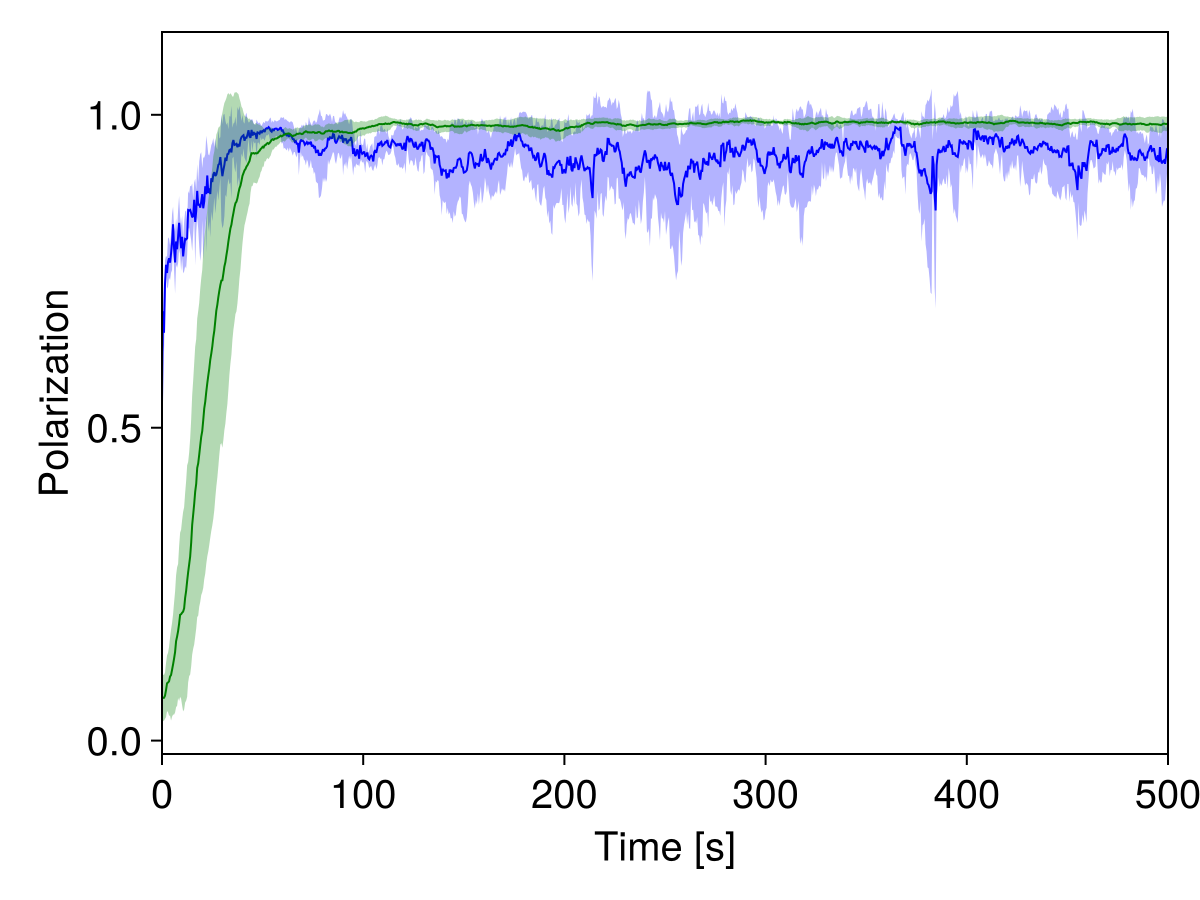
\includegraphics[width=.9\textwidth]{lj_velocity/polar20.0_oc0.5.png}}\\
			\subfloat[][]{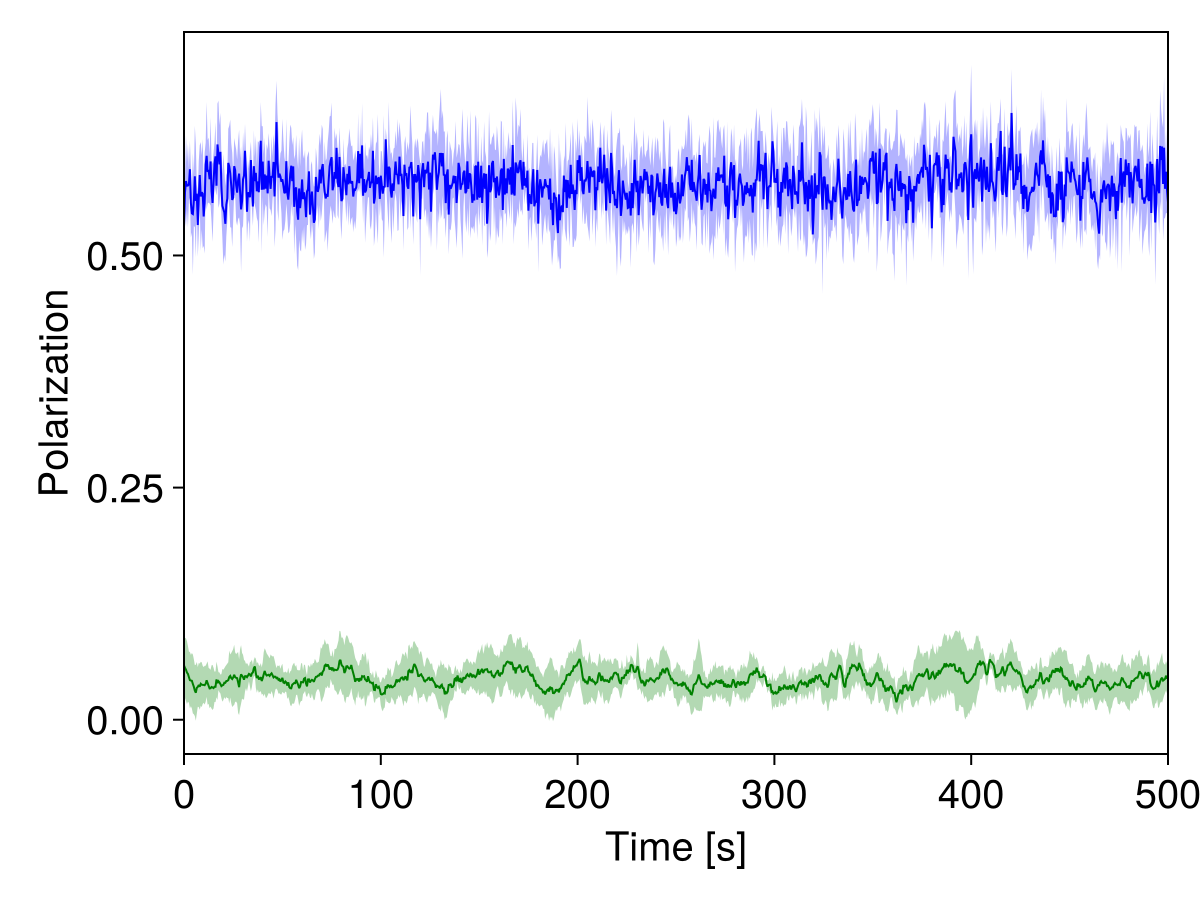
\includegraphics[width=.9\textwidth]{lj_velocity/polar10.0_oc-0.5.png}}\\
			%\captionsetup{list=false}
			\caption[]{}
		\end{figure}
		
		\begin{figure}
			\centering
			\ContinuedFloat
			\subfloat[][]{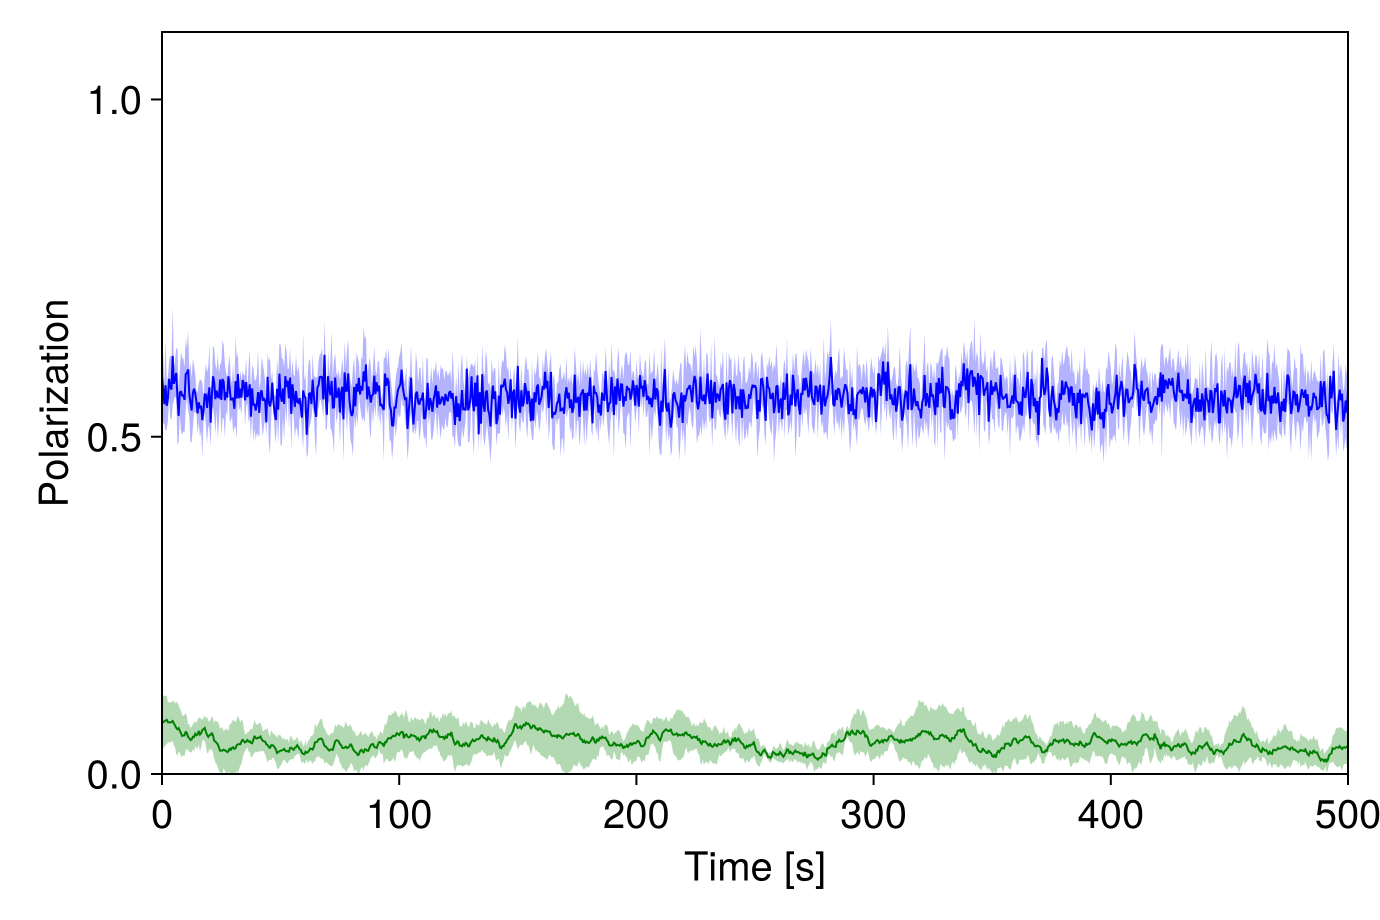
\includegraphics[width=.9\textwidth]{lj_velocity/polar20.0_oc-0.5.png}}
			\caption{(continued) Local (blue) and global (green) polarization corresponding to values of velocity and $\alpha$: (a) $v = \SI{10}{\um \per \second} \alpha = 0.5$, (b) $v = \SI{20}{\um \per \second} \alpha = 0.5$, (c) $v = \SI{10}{\um \per \second} \alpha = -0.5$, (d) $v = \SI{20}{\um \per \second} \alpha = -0.5$.}
			\label{fig:lj_velocity_pol}
		\end{figure}
		%\todo{Polarizzazione: uniforma assi y dei subplot}
		
		\begin{figure}[hbtp]
			\centering\
			\subfloat[][]{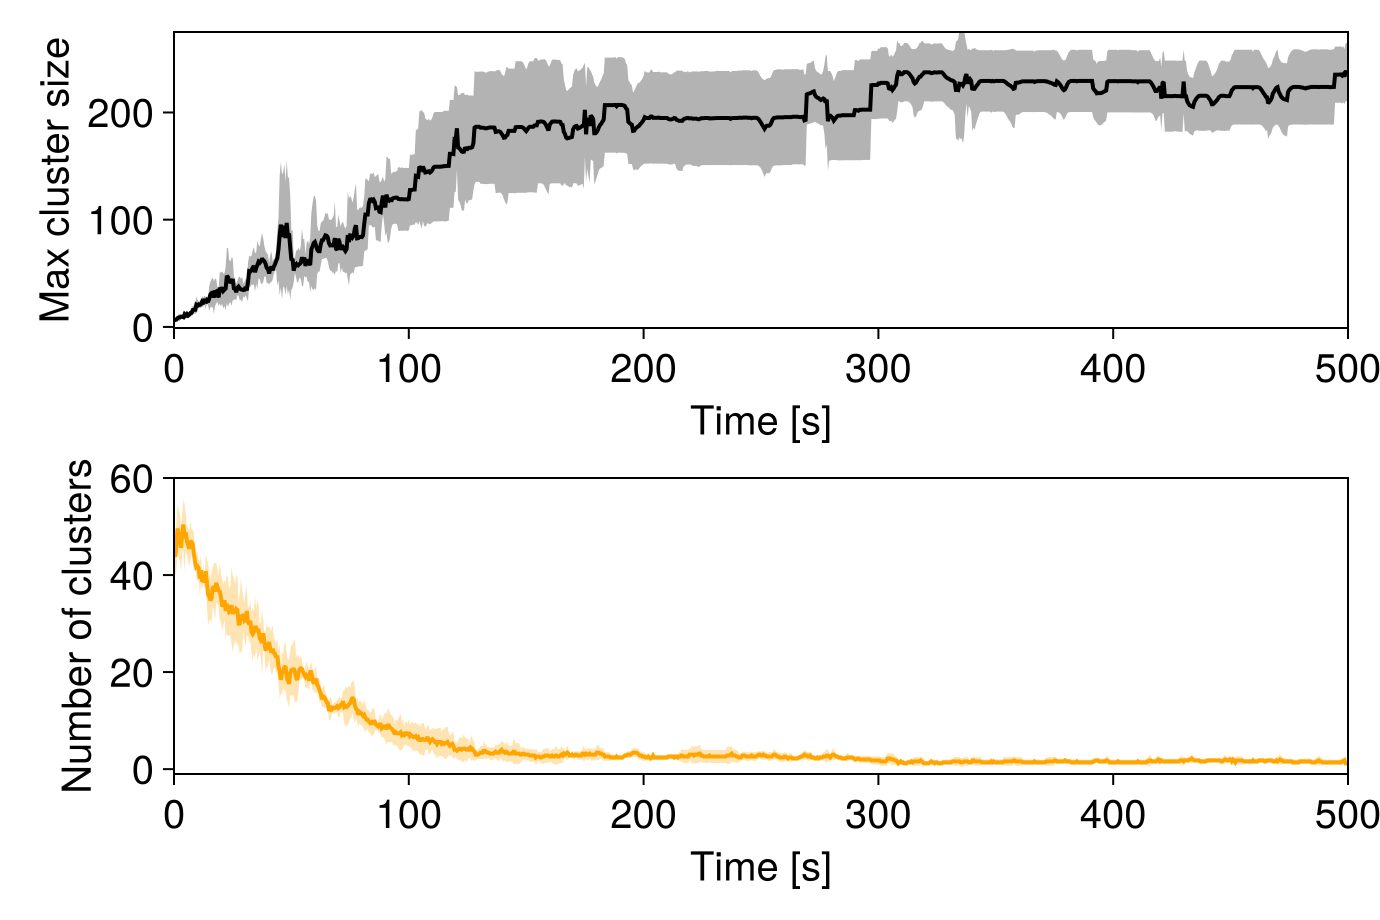
\includegraphics[width=.9\textwidth]{lj_velocity/cluster10.0_oc0.5.png}}\\
			\subfloat[][]{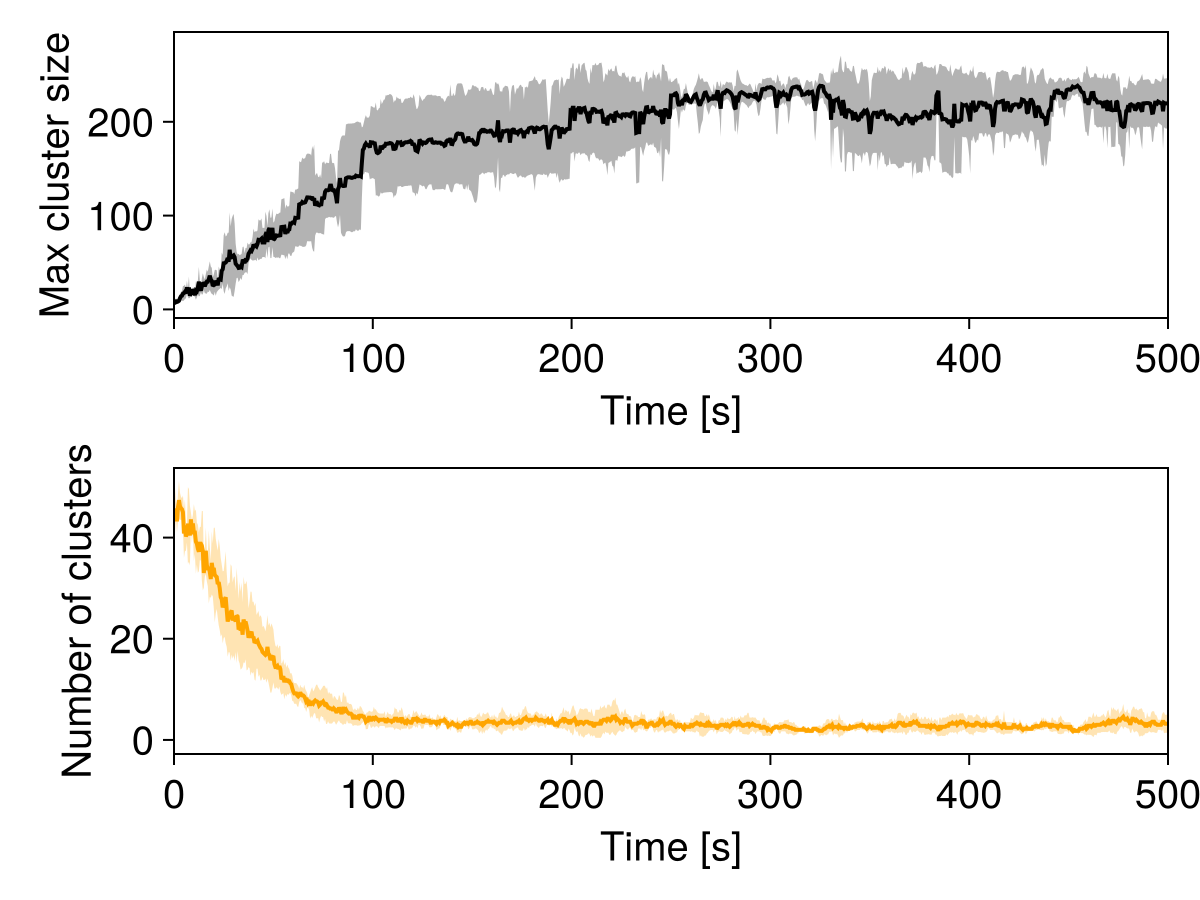
\includegraphics[width=.9\textwidth]{lj_velocity/cluster20.0_oc0.5.png}}\\
			\subfloat[][]{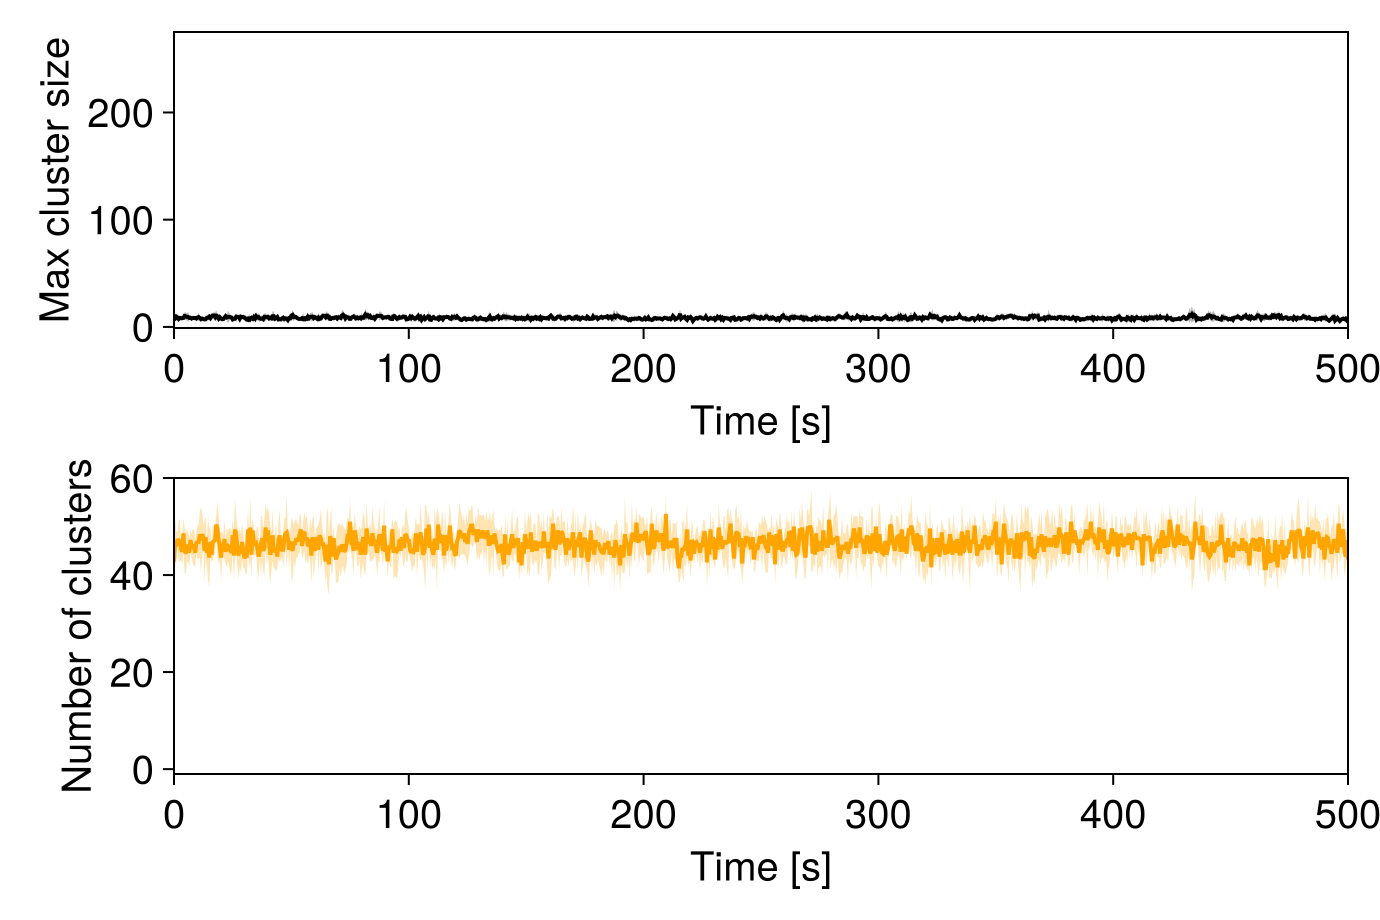
\includegraphics[width=.9\textwidth]{lj_velocity/cluster10.0_oc-0.5.png}}\\
			%\captionsetup{list=false}
			\caption[]{}
		\end{figure}
		\begin{figure}
			\centering
			\ContinuedFloat

			\subfloat[][]{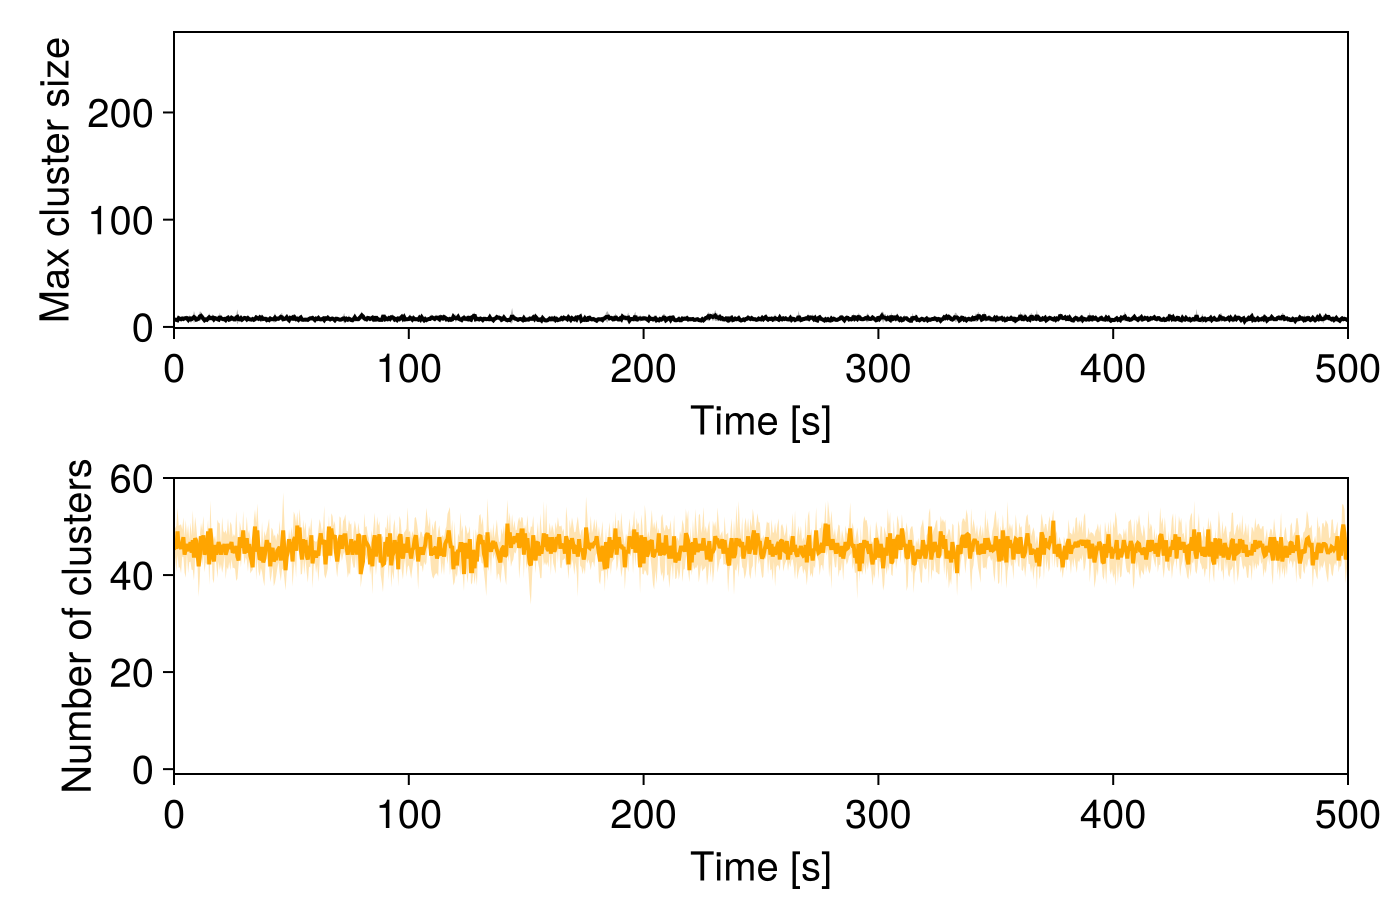
\includegraphics[width=.9\textwidth]{lj_velocity/cluster20.0_oc-0.5.png}}\\

			\caption{(continued) Maximum cluster size and number of clusters corresponding to values of velocity and $\alpha$: (a) $v = \SI{10}{\um \per \second} \alpha = 0.5$, (b) $v = \SI{20}{\um \per \second} \alpha = 0.5$, (c) $v = \SI{10}{\um \per \second} \alpha = -0.5$, (d) $v = \SI{20}{\um \per \second} \alpha = -0.5$.}
			\label{fig:lj_velocity_cluster}
		\end{figure}
		%\todo{Cluster: uniforma assi y dei subplot (sembrano leggermente diversi)}

		This can also be noticed in Figures \ref{fig:lj_velocity_situa} and \ref{fig:lj_velocity_cluster}, where, when the off center position is on the back, velocity tends to hinder clustering, leading to a more sparse final situation. 
		We anticipate the following explanation for this: for same velocity particles, head to tail collision is unlikely because interacting positions of these particles will always be at a distance $> 2R$, where interactions are relatively weak.
		Radial distribution functions in Figure \ref{fig:lj_velocity_rdf} show how a particles which swim with their interacting position on the back tend to develop less long range order, regardless their velocity.
		
		\begin{figure}[hbtp]
			\centering\
			\subfloat[][]{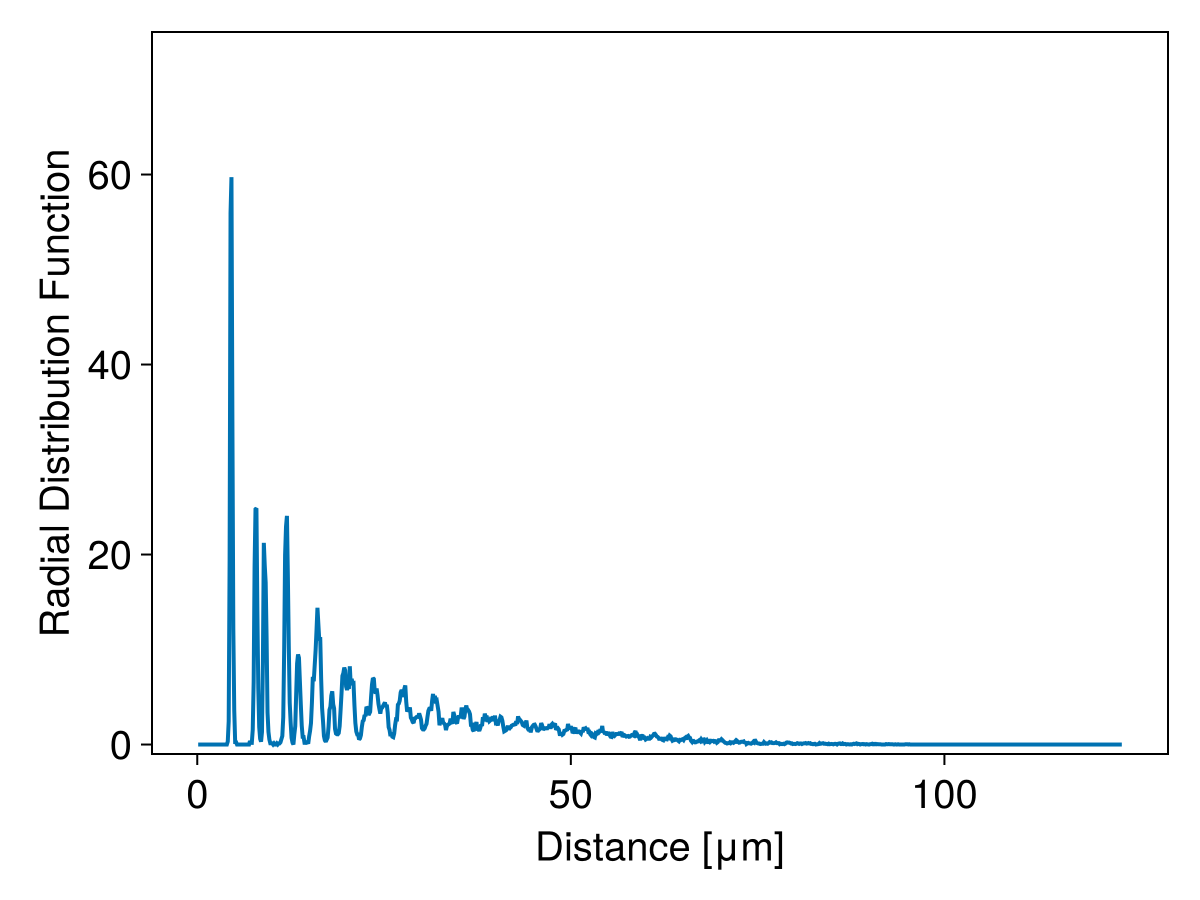
\includegraphics[width=.9\textwidth]{lj_velocity/rdf10.0_oc0.5.png}}\\
			\subfloat[][]{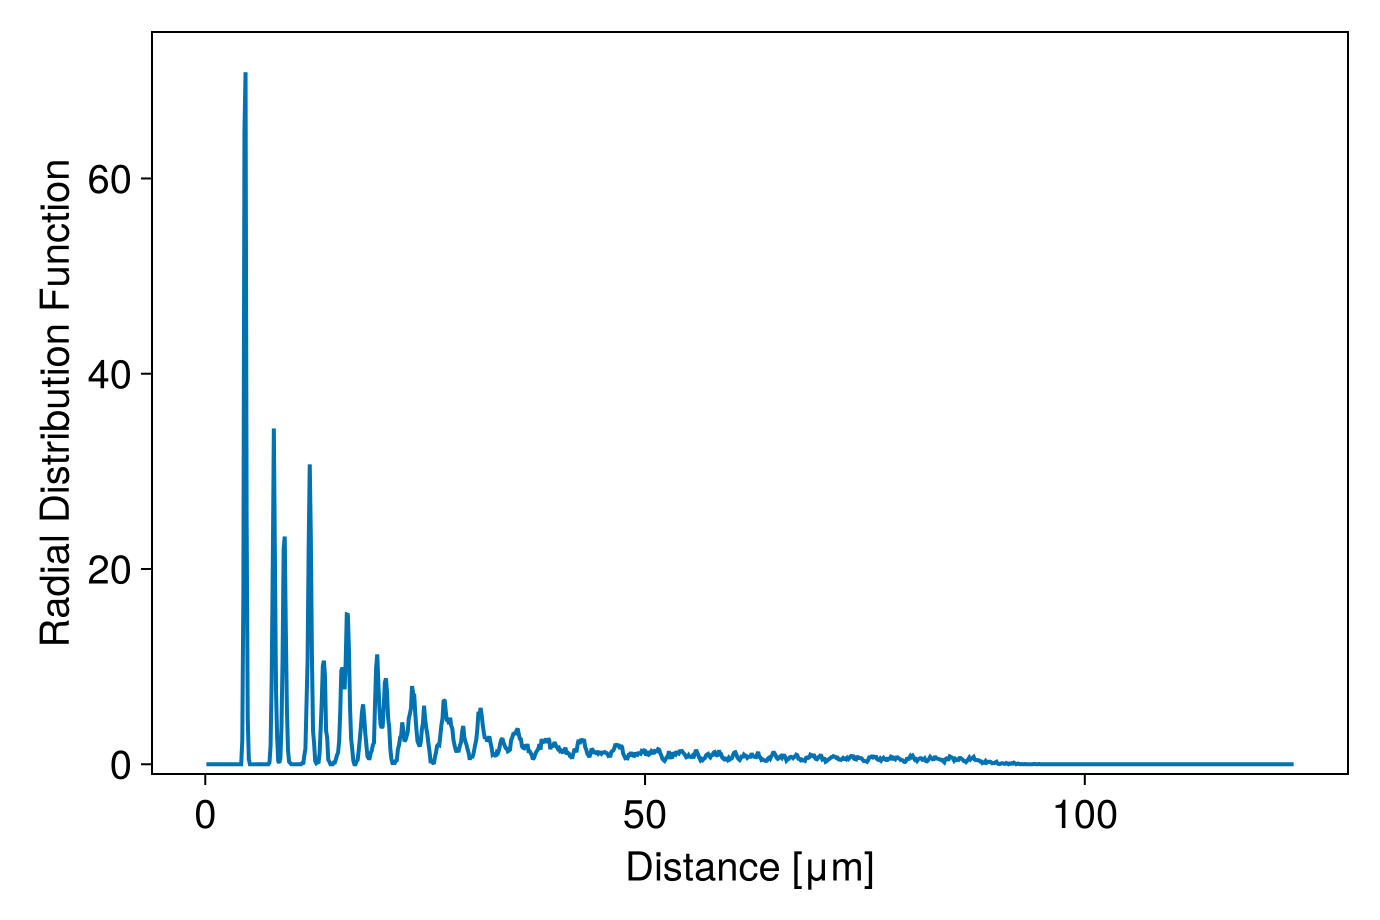
\includegraphics[width=.9\textwidth]{lj_velocity/rdf20.0_oc0.5.png}}\\
			\subfloat[][]{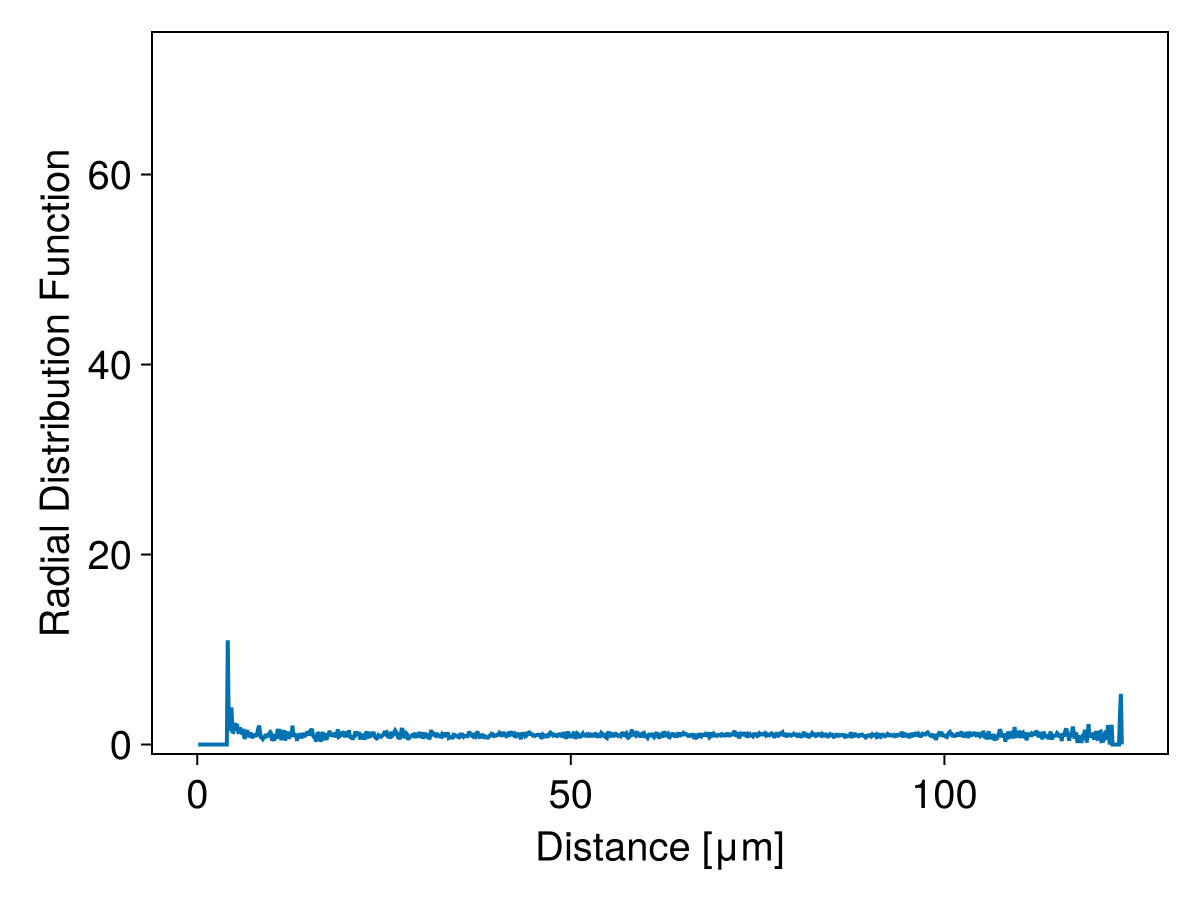
\includegraphics[width=.9\textwidth]{lj_velocity/rdf10.0_oc-0.5.png}}
			%\captionsetup{list=false}
			\caption[]{}
		\end{figure}
		\begin{figure}
			\centering
			\ContinuedFloat
			\subfloat[][]{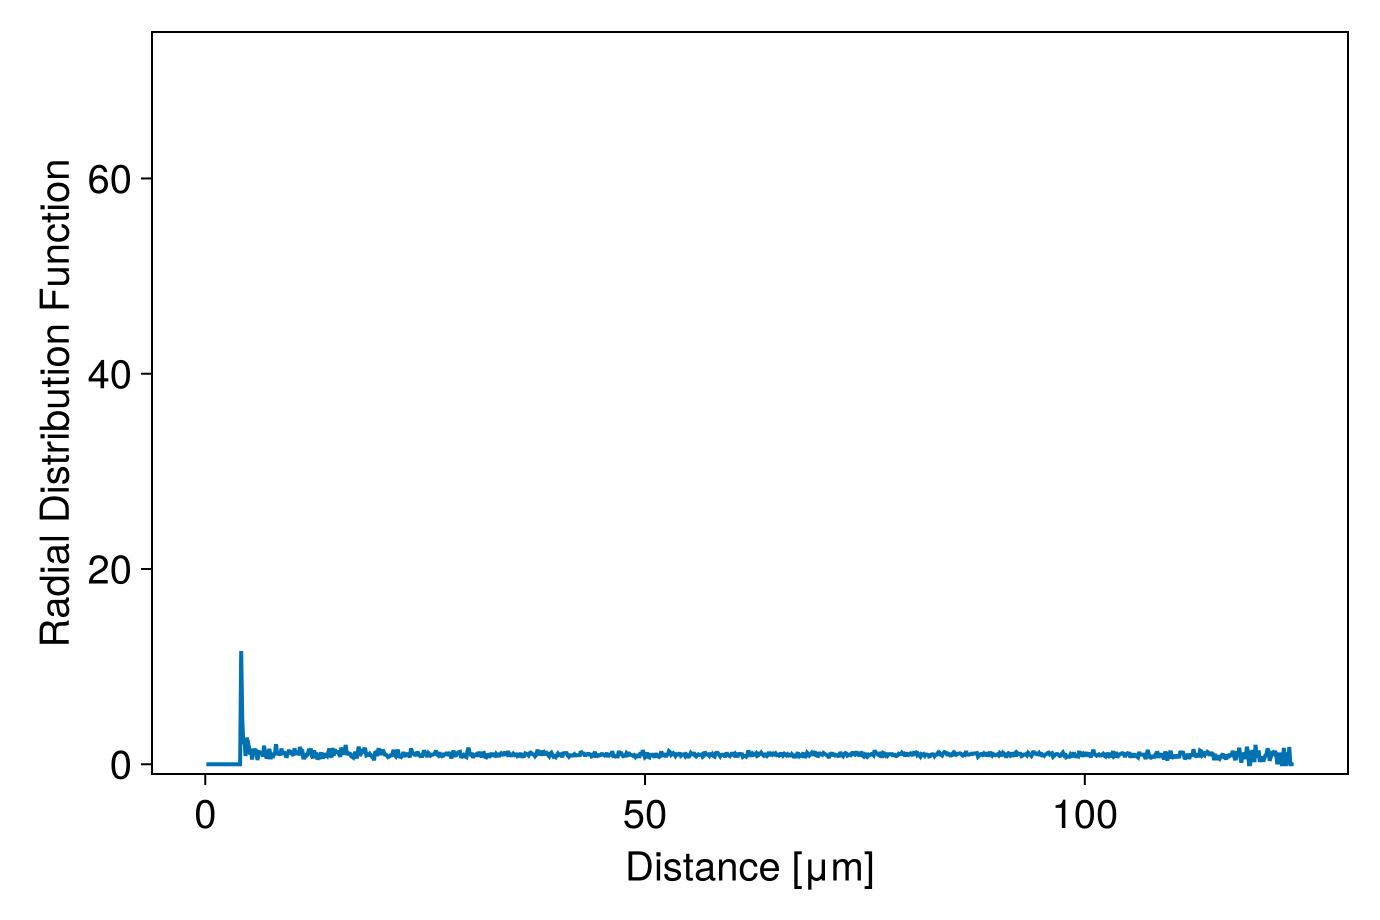
\includegraphics[width=.9\textwidth]{lj_velocity/rdf20.0_oc-0.5.png}}\\
			
			\caption{(continued) Radial distribution function at last instant of simulation corresponding to values of velocity and $\alpha$: (a) $v = \SI{10}{\um \per \second} \alpha = 0.5$, (b) $v = \SI{20}{\um \per \second} \alpha = 0.5$, (c) $v = \SI{10}{\um \per \second} \alpha = -0.5$, (d) $v = \SI{20}{\um \per \second} \alpha = -0.5$.}
			\label{fig:lj_velocity_rdf}
		\end{figure}

		\subsection{Velocity Distribution}
		\label{veldist}
		A simple way to add experiments inspired complexity into the model is to initialize particles with different self propulsion velocity. 
		This way collisions are more likely and in a greater variety of directions' configurations.
		In this sections, we used the standard potential with an off center parameter $\alpha = 0.5$.
		
		To implement different velocities we used normal distribution, keeping the mean constant at \SI{10}{\um \per \second} while changing the standard deviation in \qtylist{1; 2; 5; 10}{\um \per \second}.
		To avoid having particles that swim backwards with respect to their self propulsion direction, the distribution was truncated at zero.
		
		Considerations about collisions could lead to the expectation that, with a velocity distribution, particles will cluster more easily in a MIPS fashion.
		In fact, both cluster size and $g(r)$ (Figures \ref{fig:lj_vdist_clust} and \ref{fig:lj_vdist_rdf}) show how adding different velocities to the system tends to hinder packing, leading in the end to a more sparse system, compared to a constant velocity case.
		
		From the polarization standpoint, increasing the broadness of the velocity distribution tends to slightly reduce the amount of total alignment in the system, while local polarization remains higher. 
		A remarkable observation is that although in our study we showed that alignment and clustering are often related, here a drastic downfall of clustering does not reflect in a big difference in polarization, resulting in a sparse system with a high alignment.
		This is immediately noticeable, in addition to the graphs in Figures \ref{fig:lj_vdist_pol} and \ref{fig:lj_vdist_clust}, in the snapshot in panel (d) of Figure \ref{fig:lj_vdist_situa}.
		In line with previous section, faster velocities make transient times shorter.
		These results are relevant, since alignment in packed ABPs systems is a well known fact \cite{caprini_spontaneous_2020}, while we observed that faster particles tend to align slower ones in a sparse configuration as well, when little or no clustering takes place.
		
		\begin{figure}[htp]
			\centering\
			\subfloat[][]{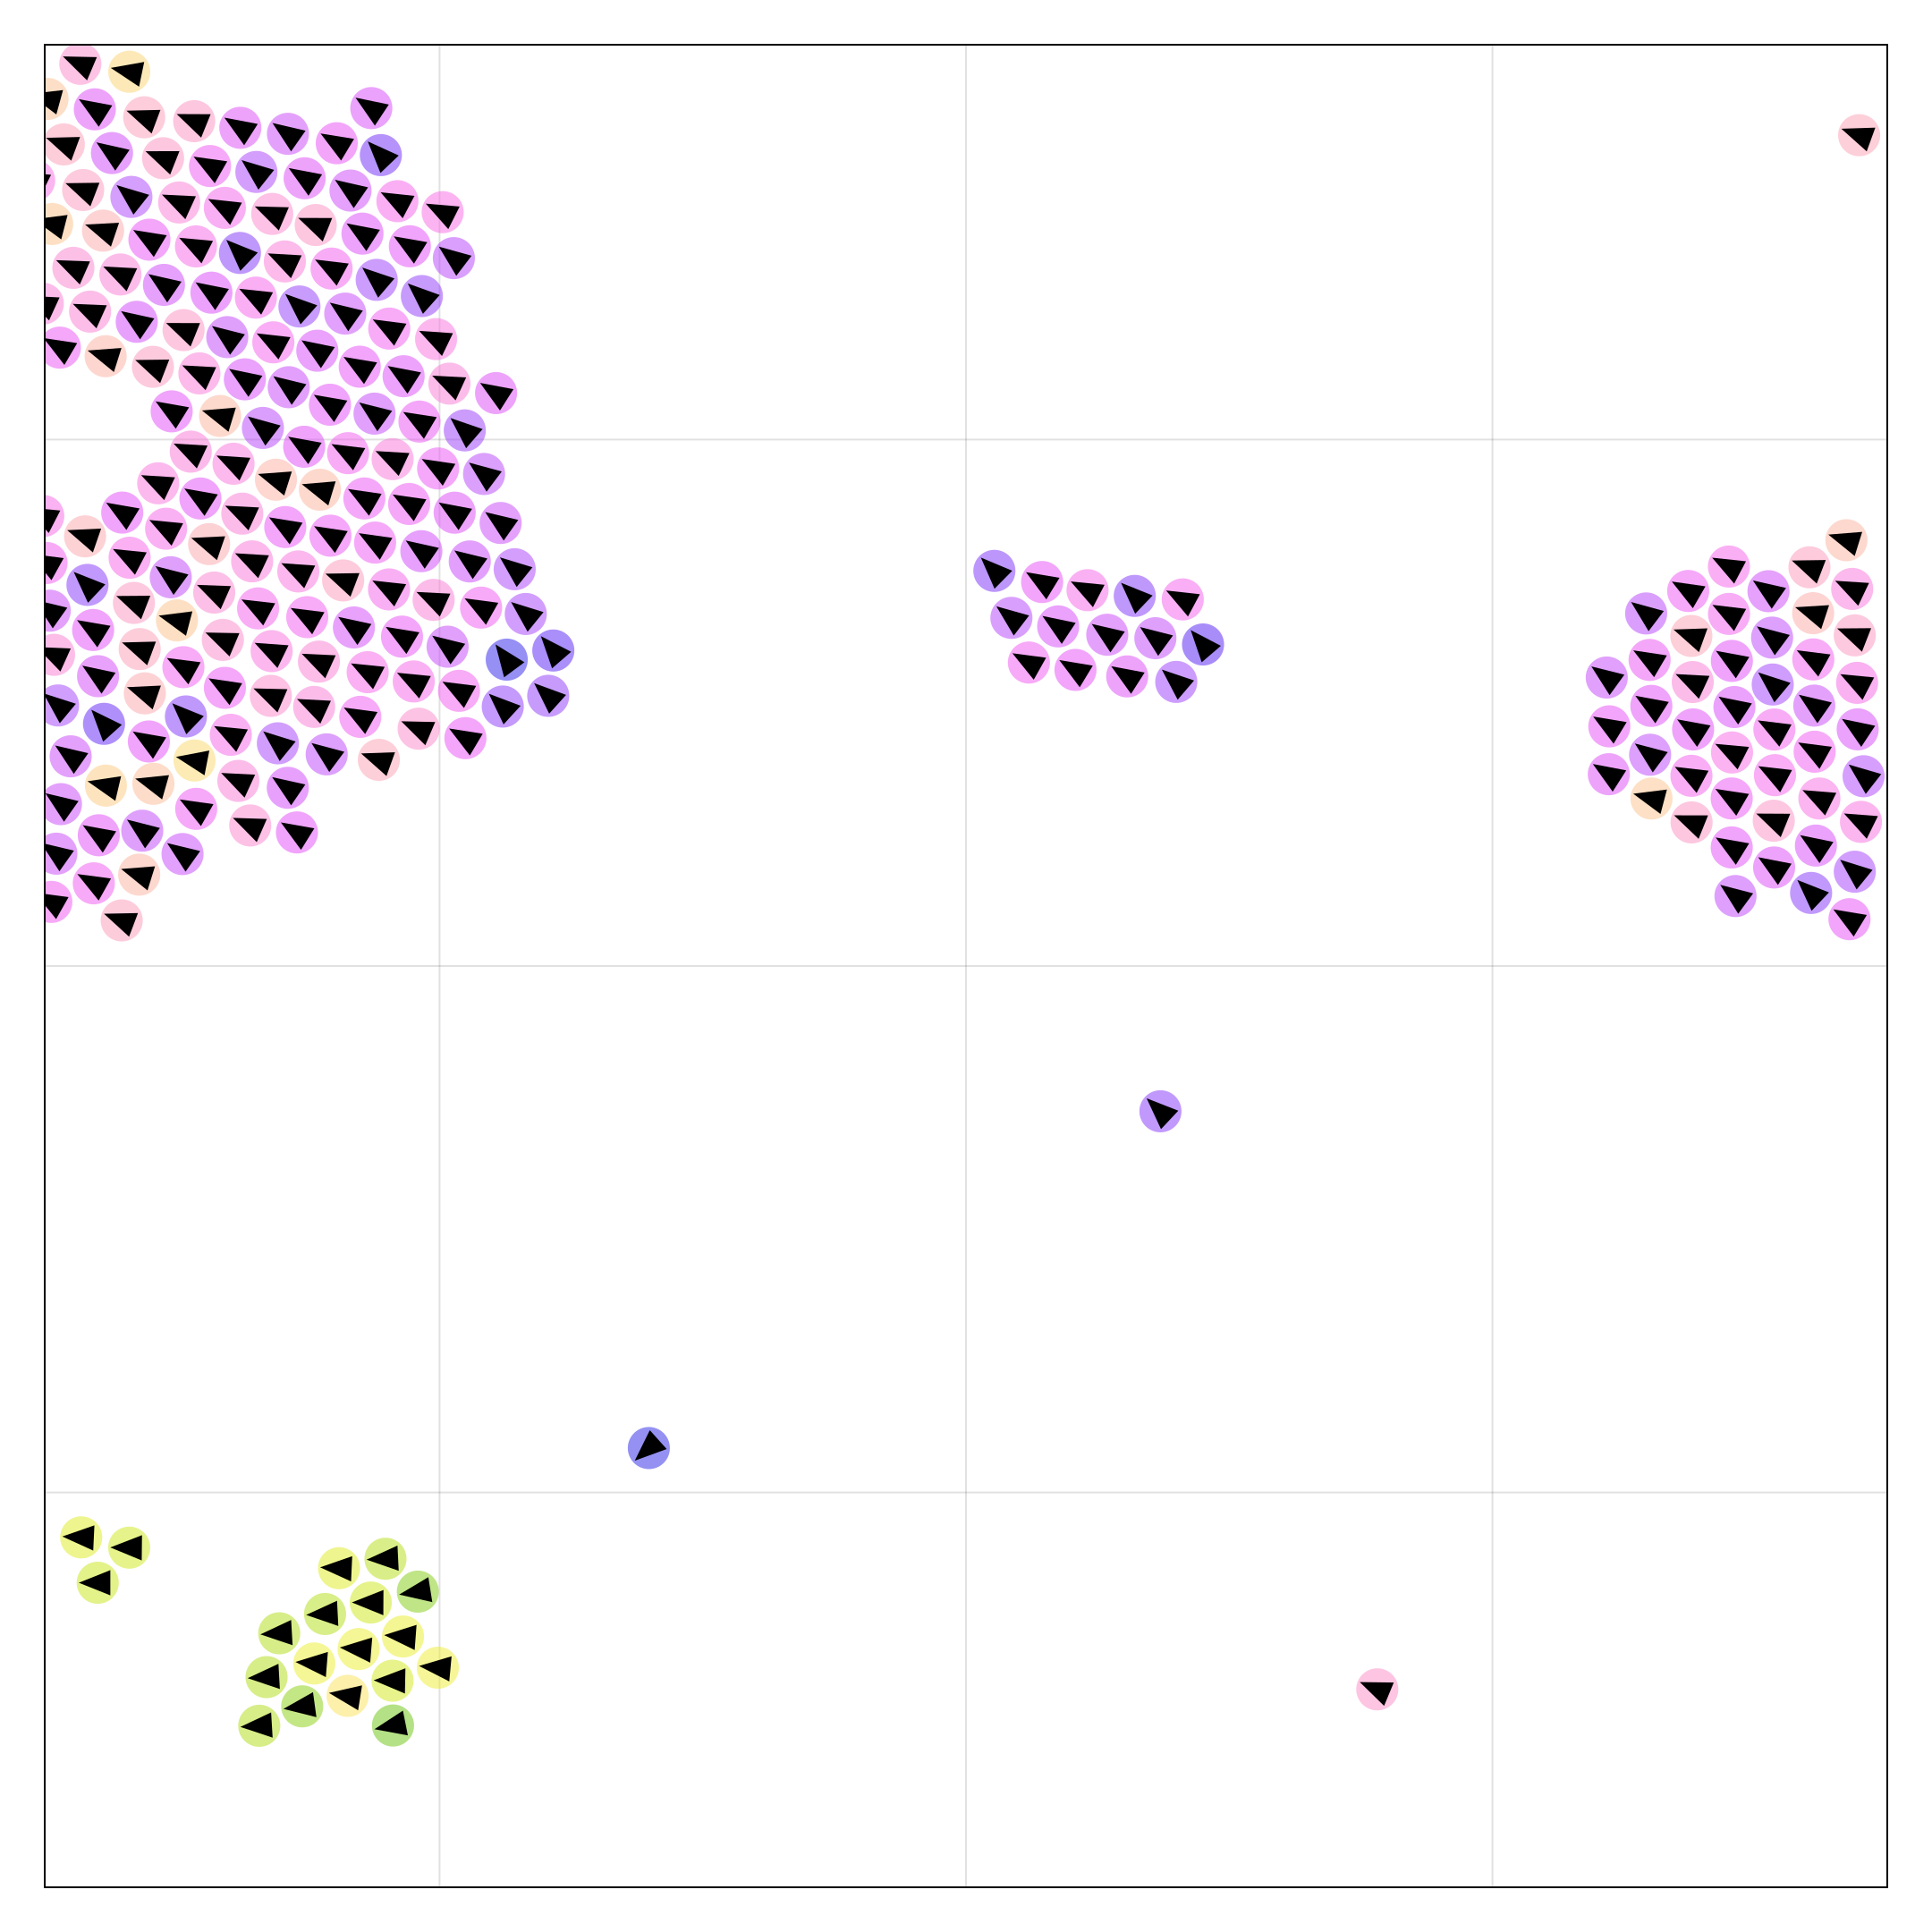
\includegraphics[width=.5\textwidth]{lj_vdist/situa1.0.png}}
			\subfloat[][]{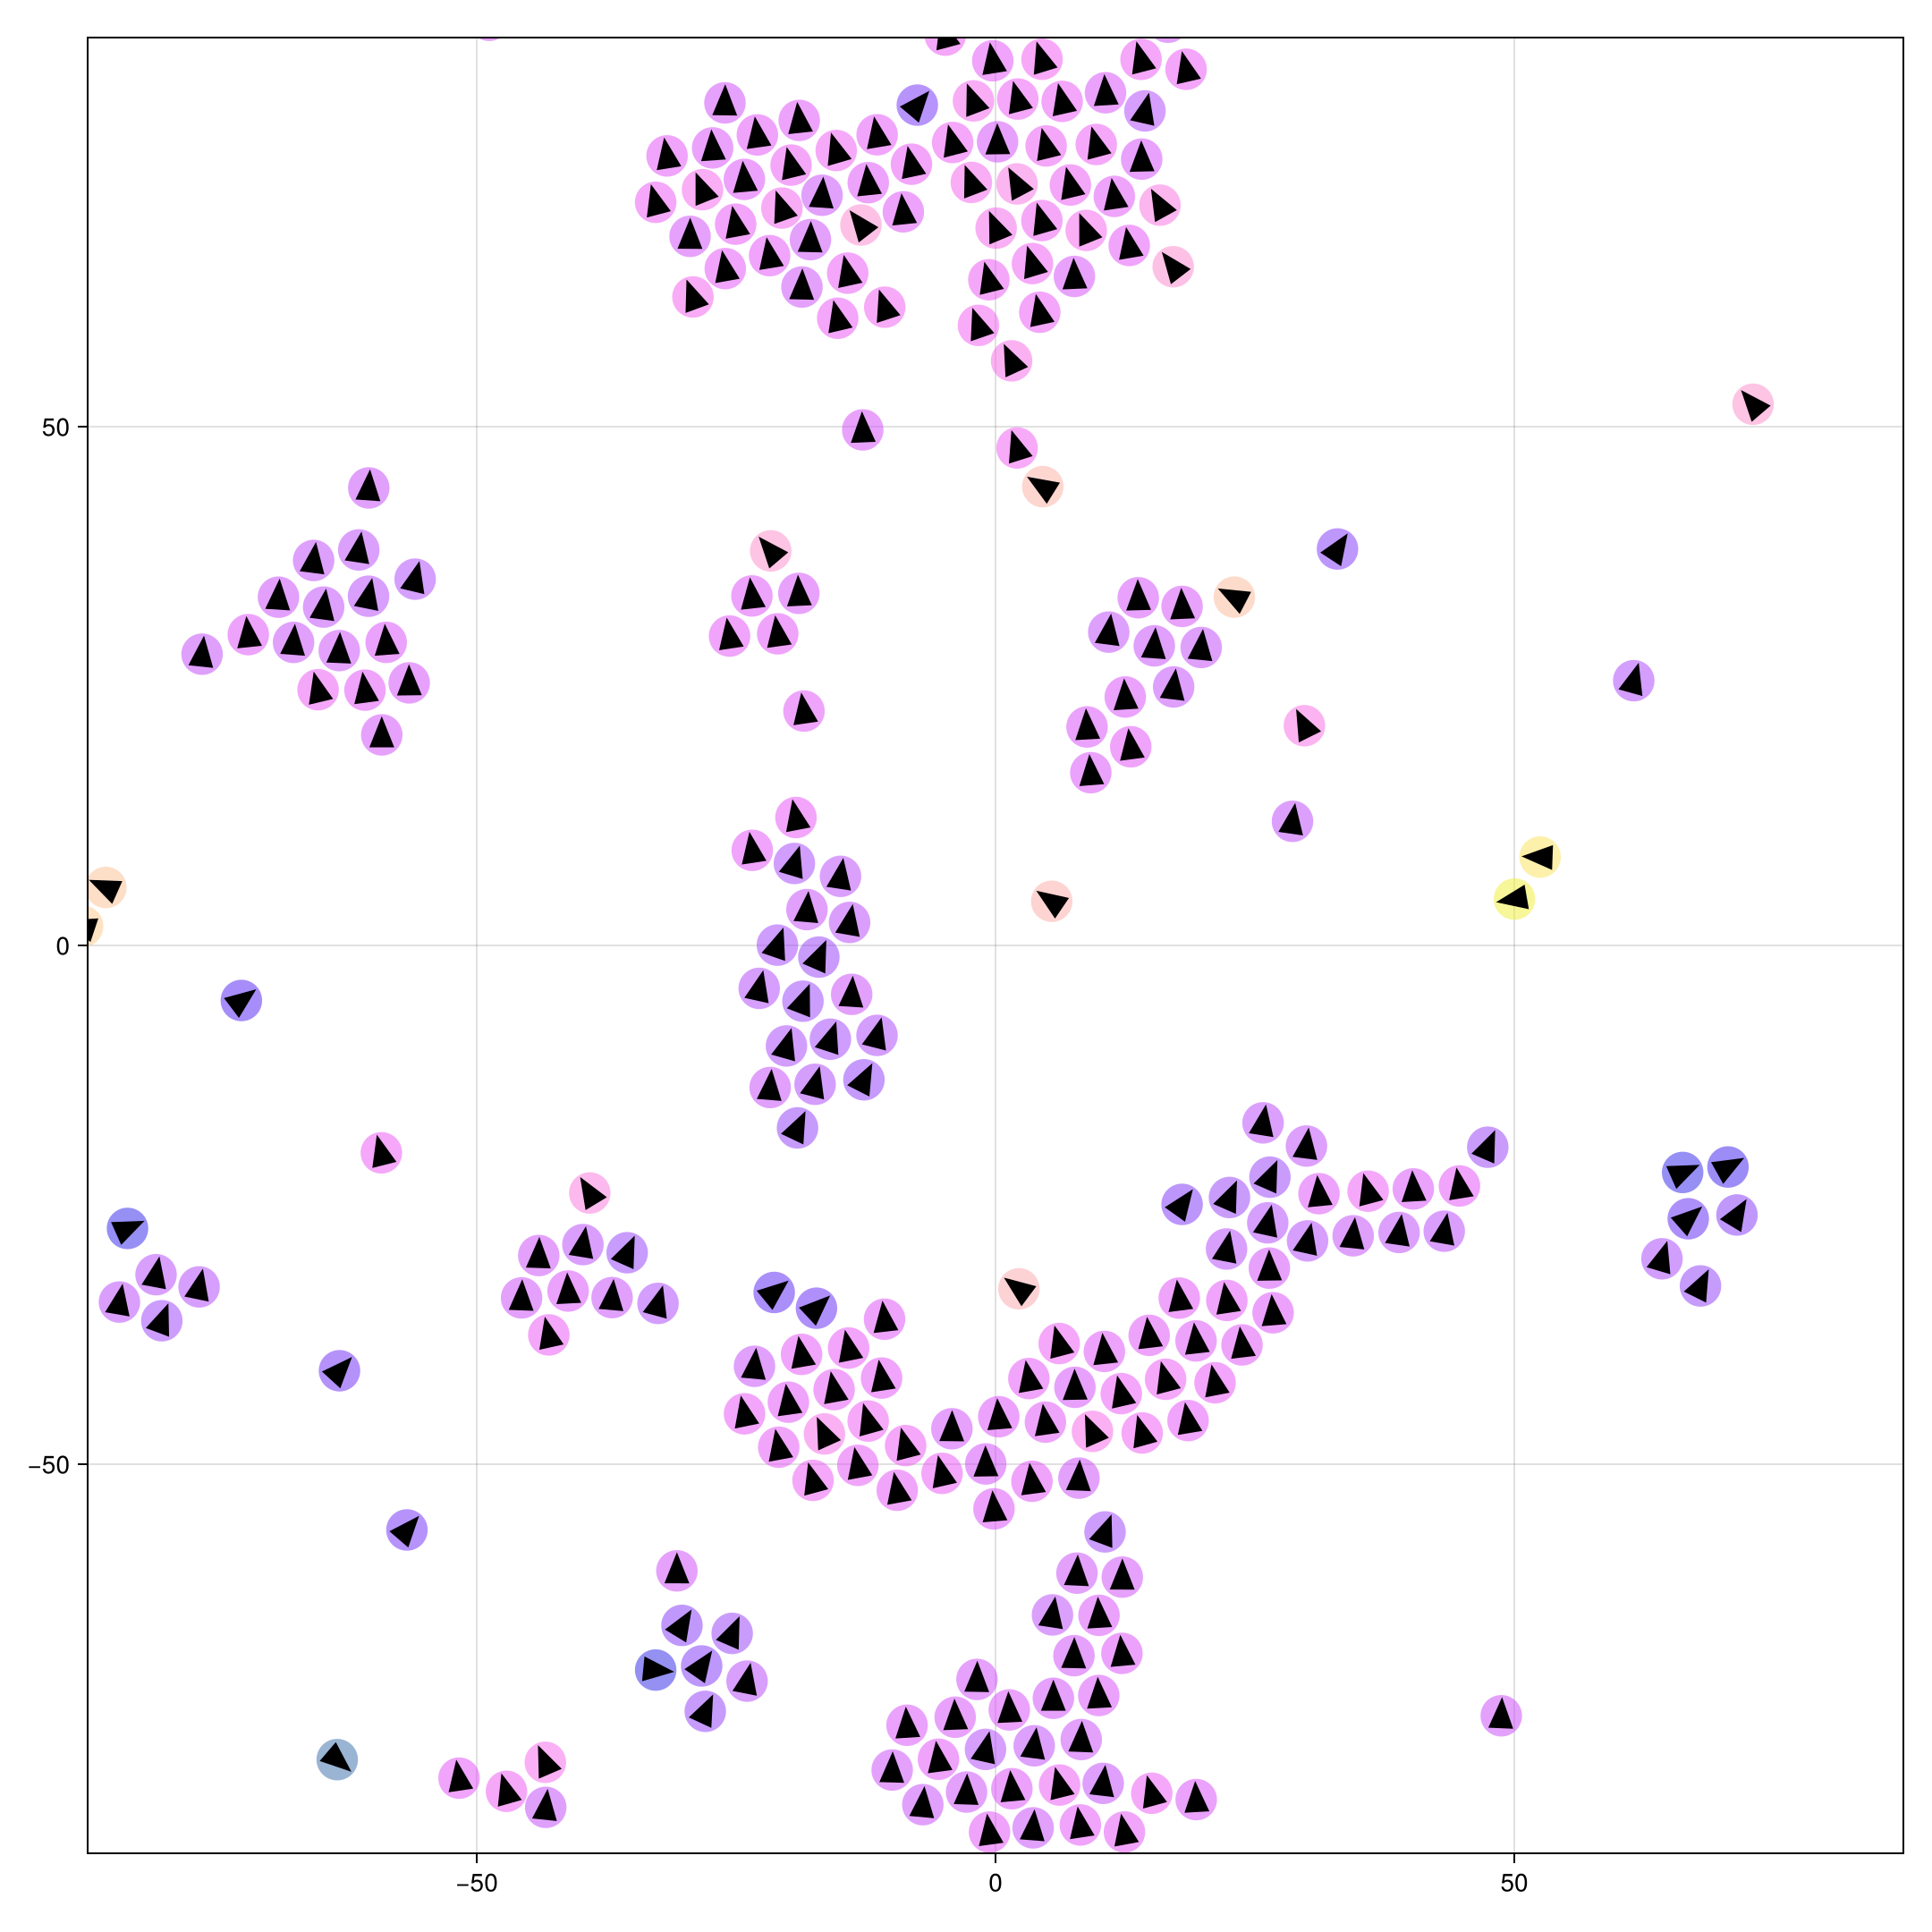
\includegraphics[width=.5\textwidth]{lj_vdist/situa2.0.png}}\\
			\subfloat[][]{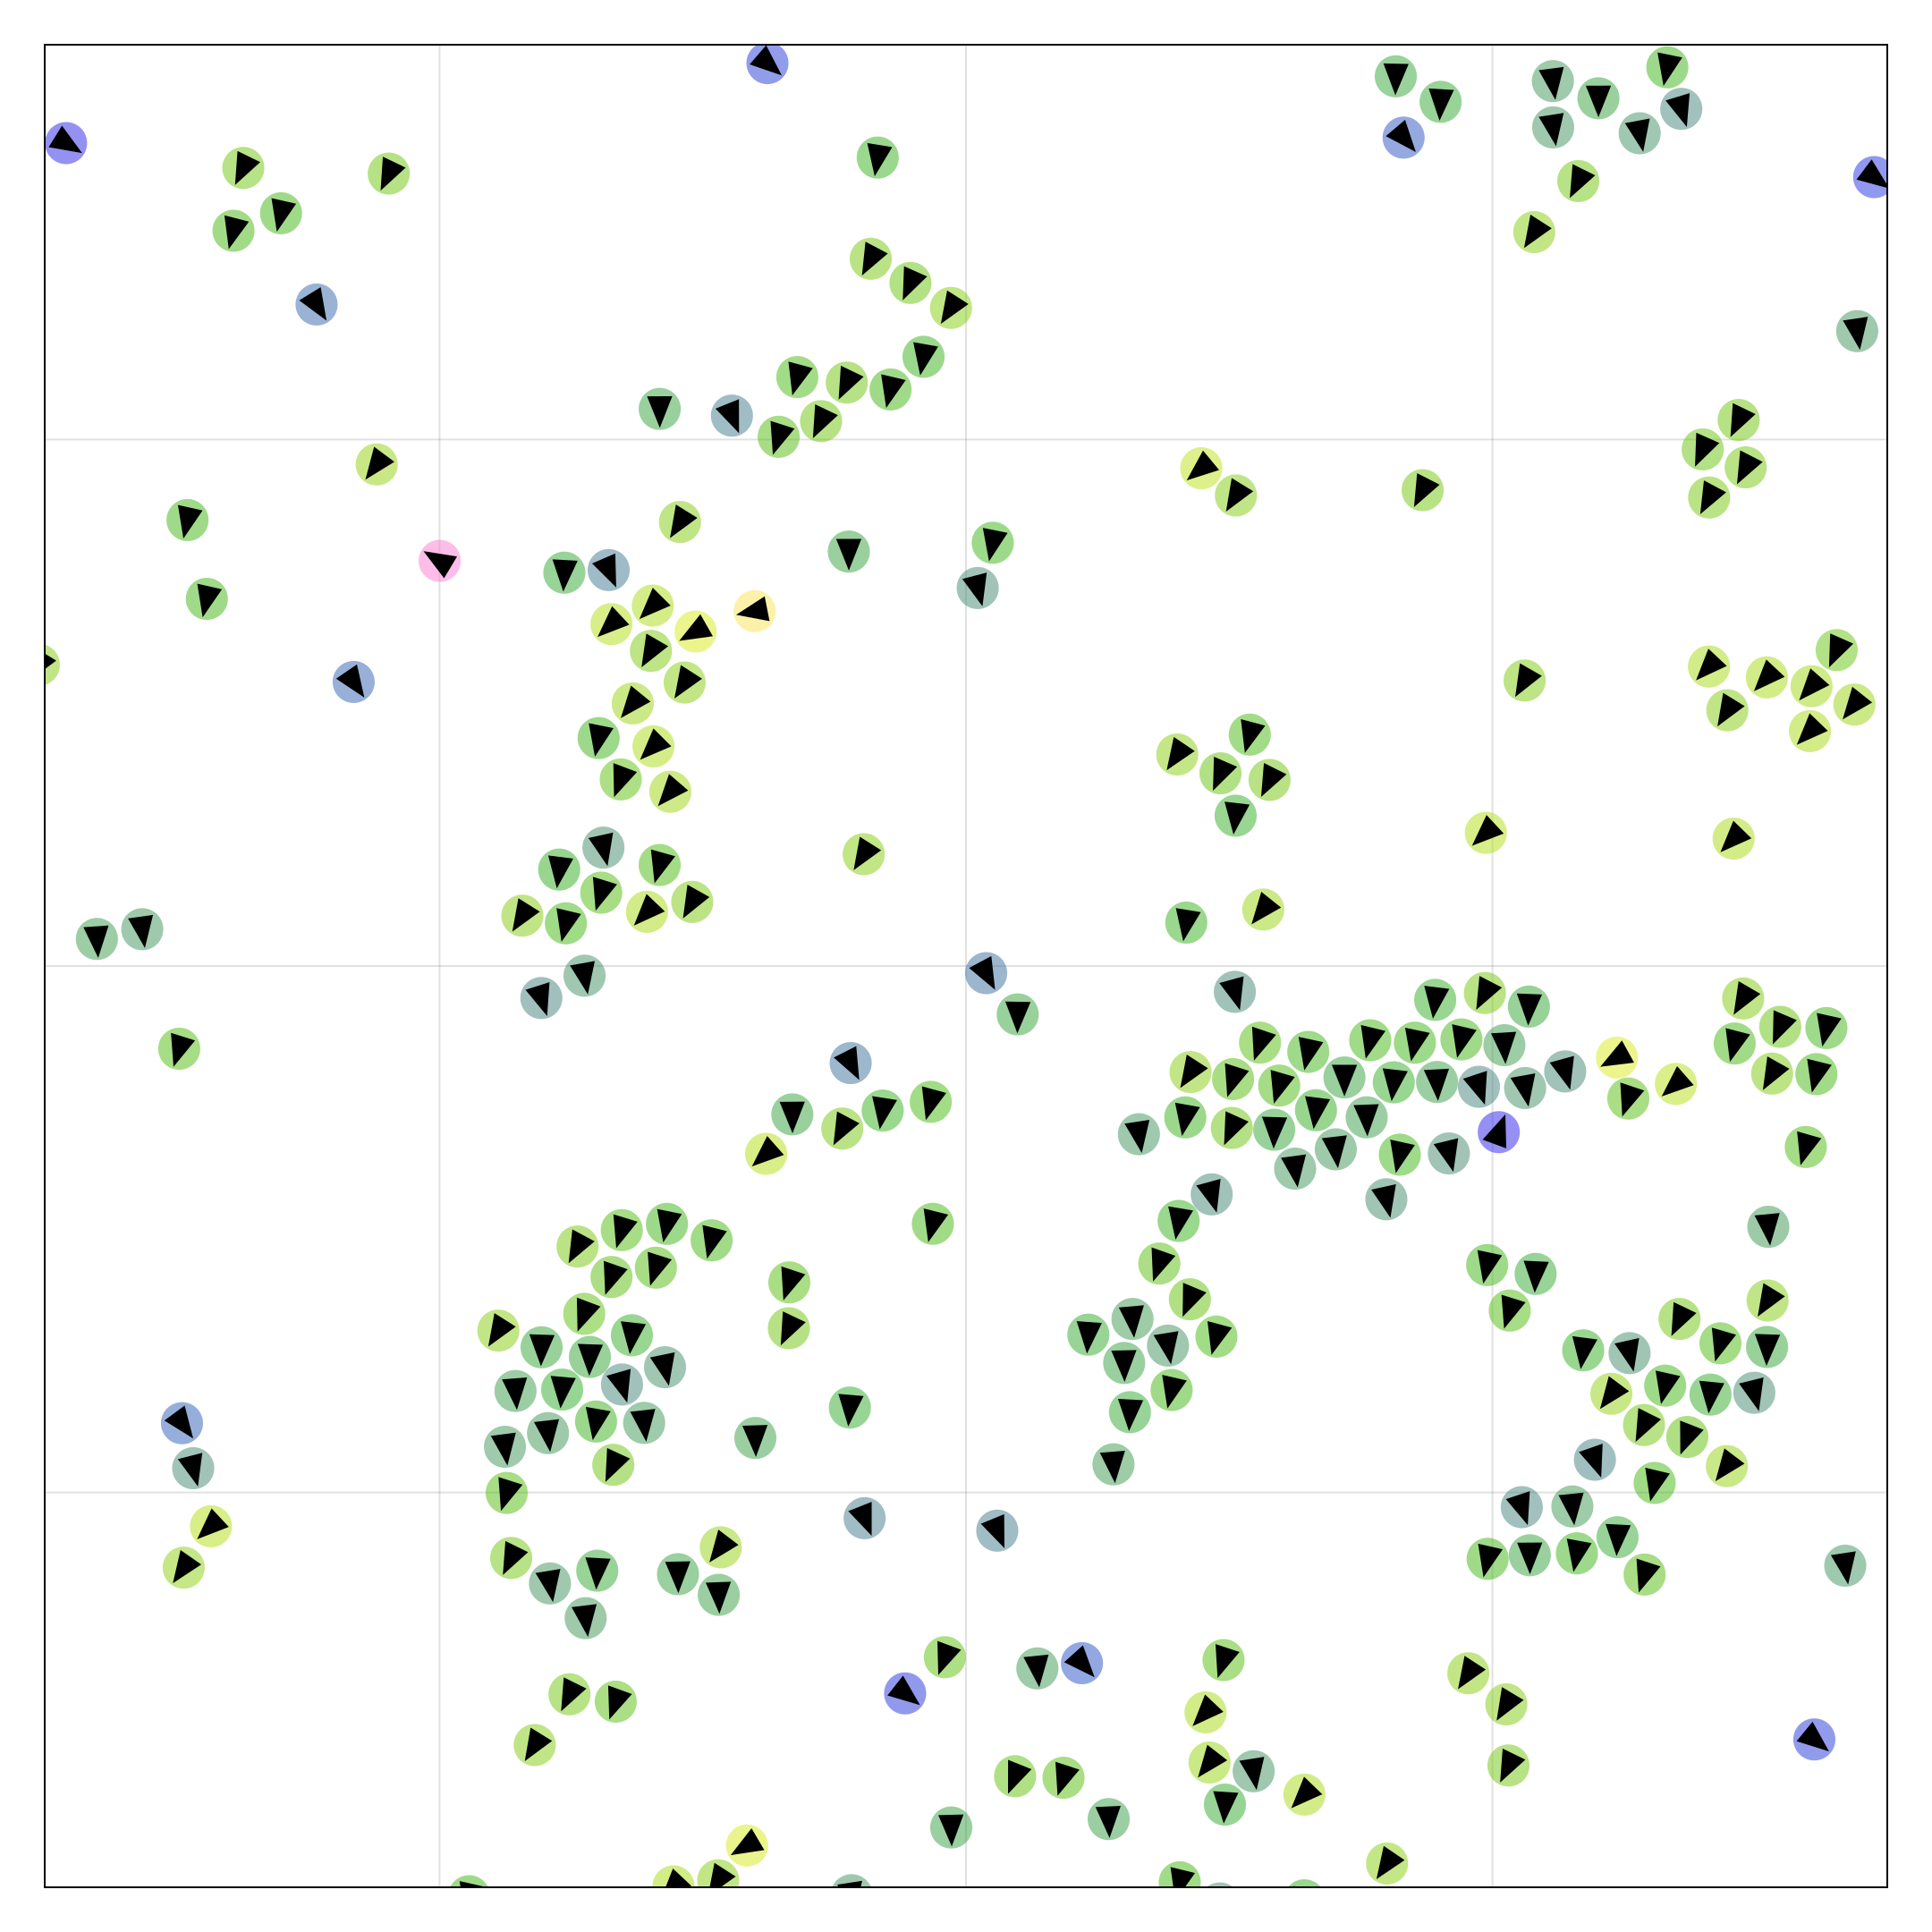
\includegraphics[width=.5\textwidth]{lj_vdist/situa5.0.png}}
			\subfloat[][]{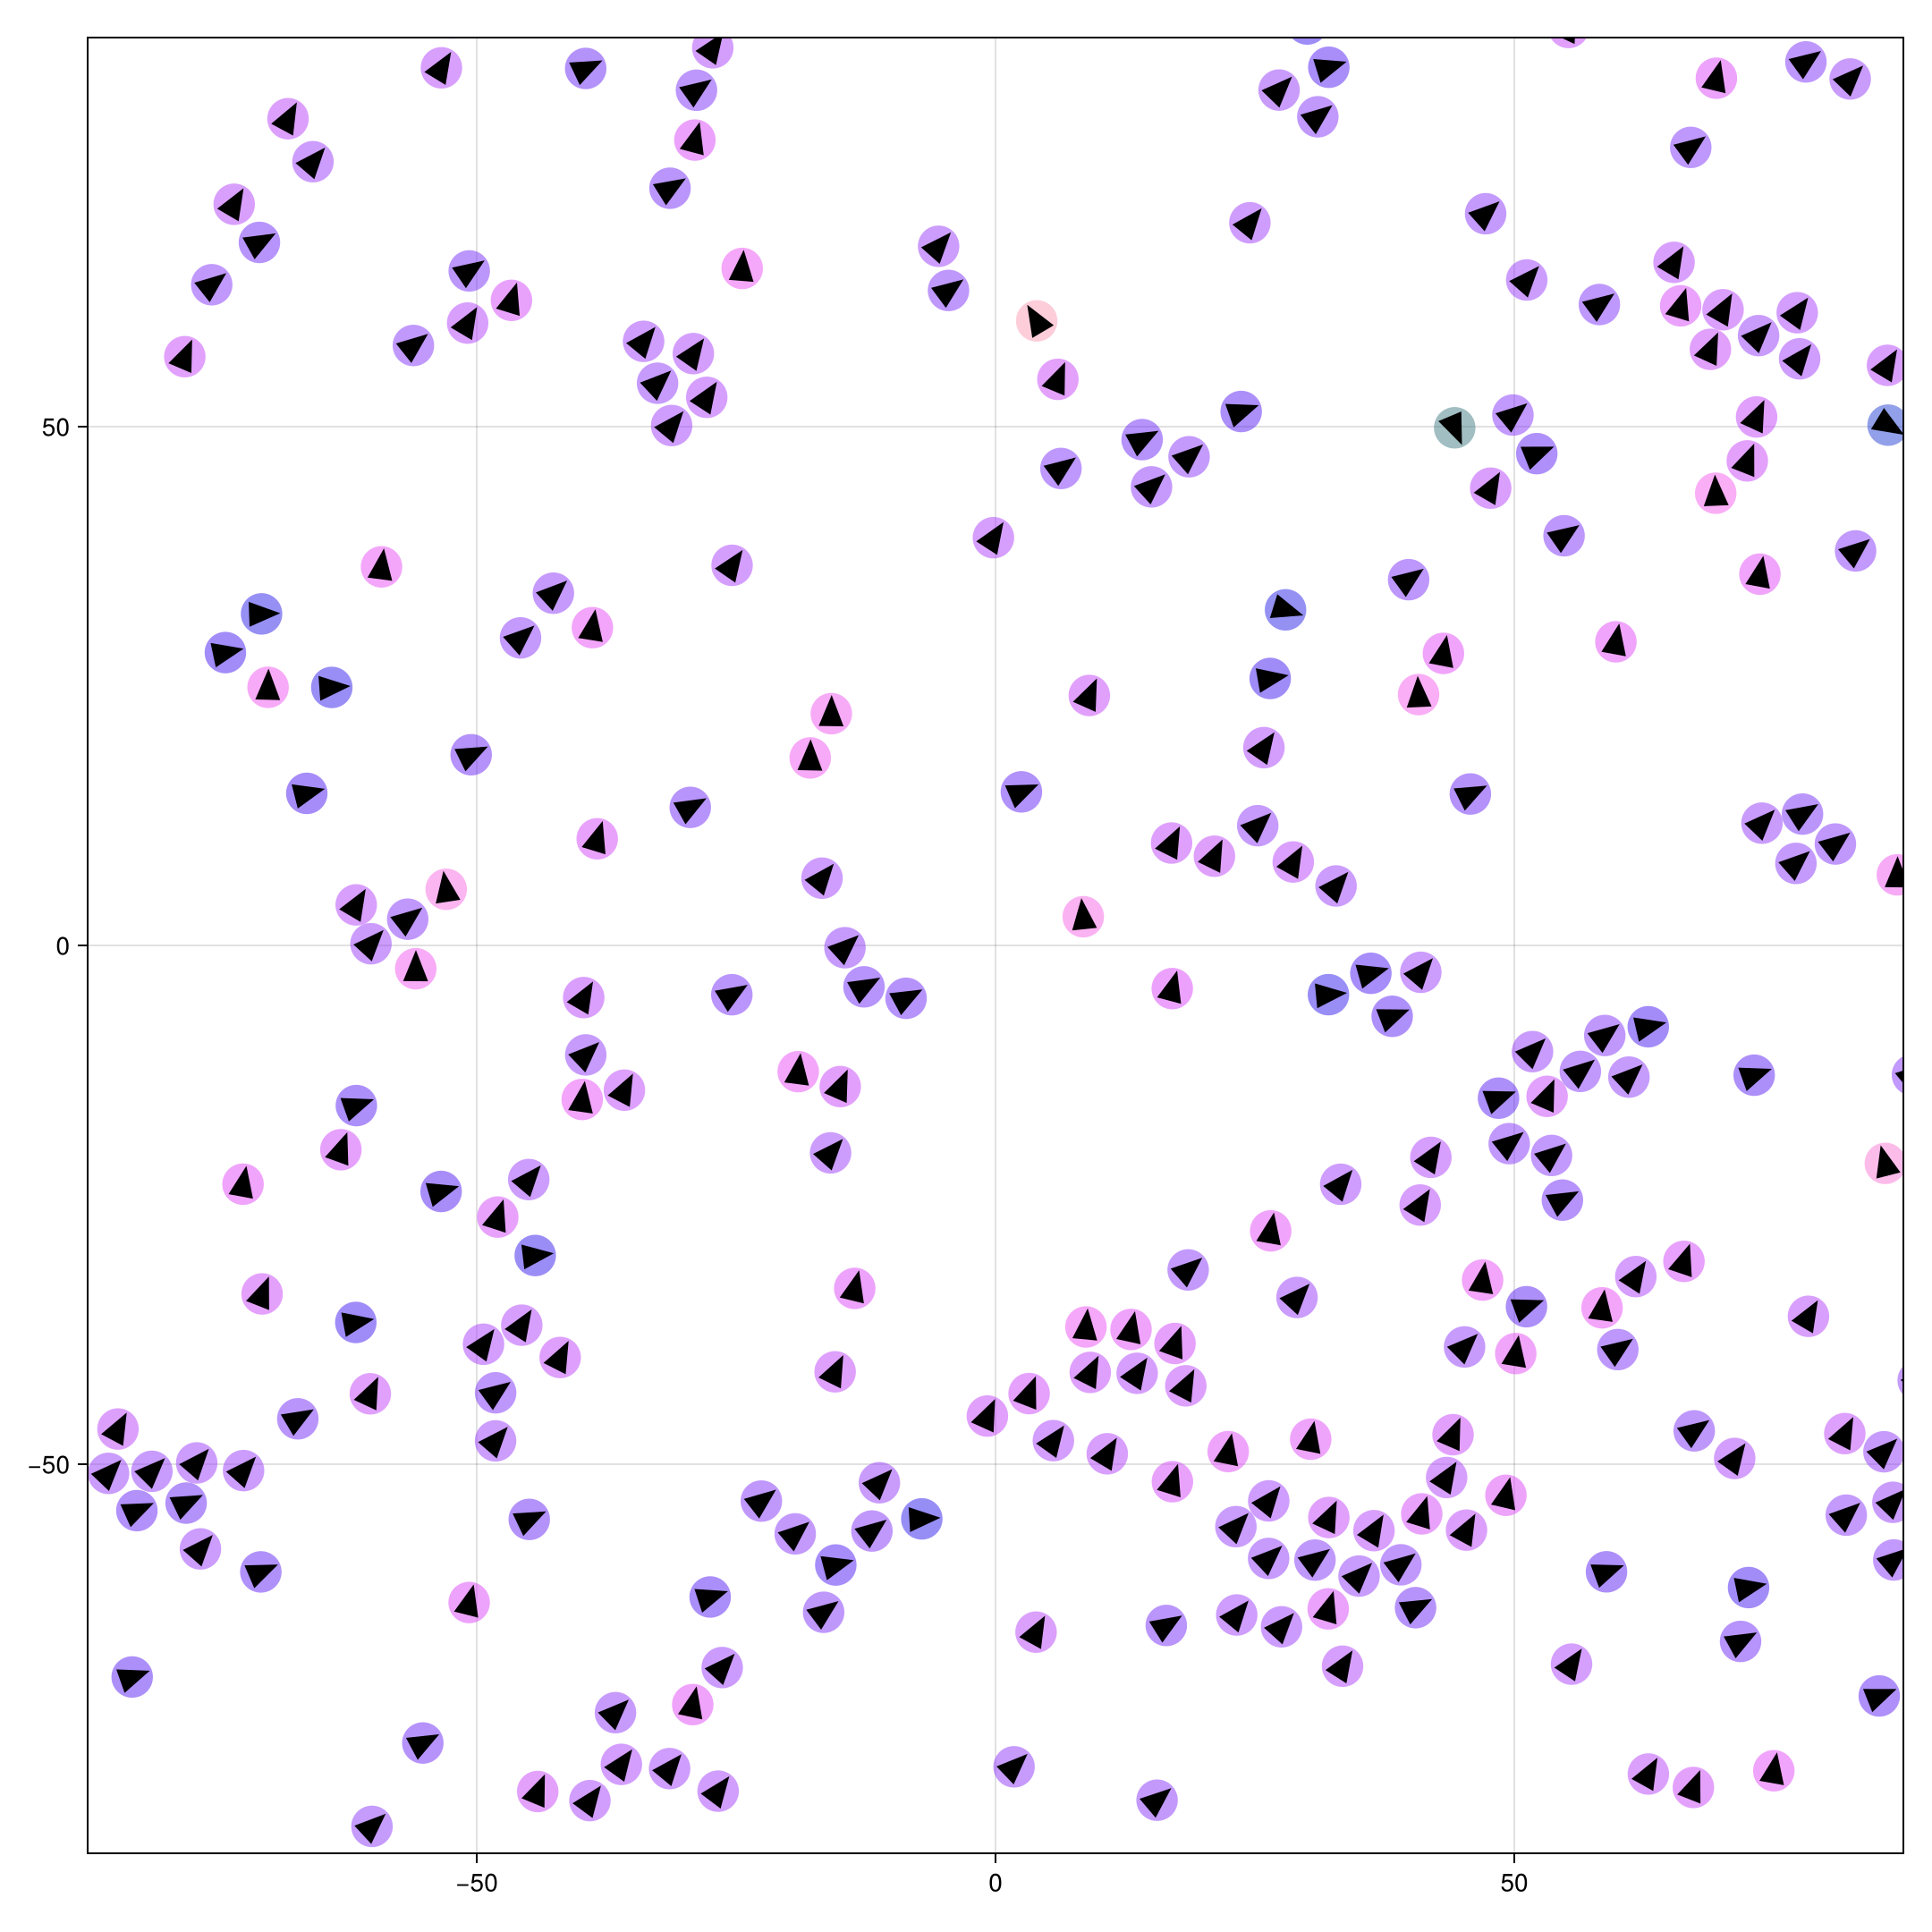
\includegraphics[width=.5\textwidth]{lj_vdist/situa10.0.png}}\\
			
			\caption{Representative simulation snapshots for a normal velocity distribution with $\mu = \SI{10}{\um\per\second}$ and standard deviation: (a) $\sigma = \SI{1}{\um\per\second}$, (b) $\sigma = \SI{2}{\um\per\second}$, (c) $\sigma = \SI{5}{\um\per\second}$, (d) $\sigma = \SI{10}{\um\per\second}$}
			\label{fig:lj_vdist_situa}
		\end{figure}
		
		\begin{figure}[htp]
			\centering\
			\subfloat[][]{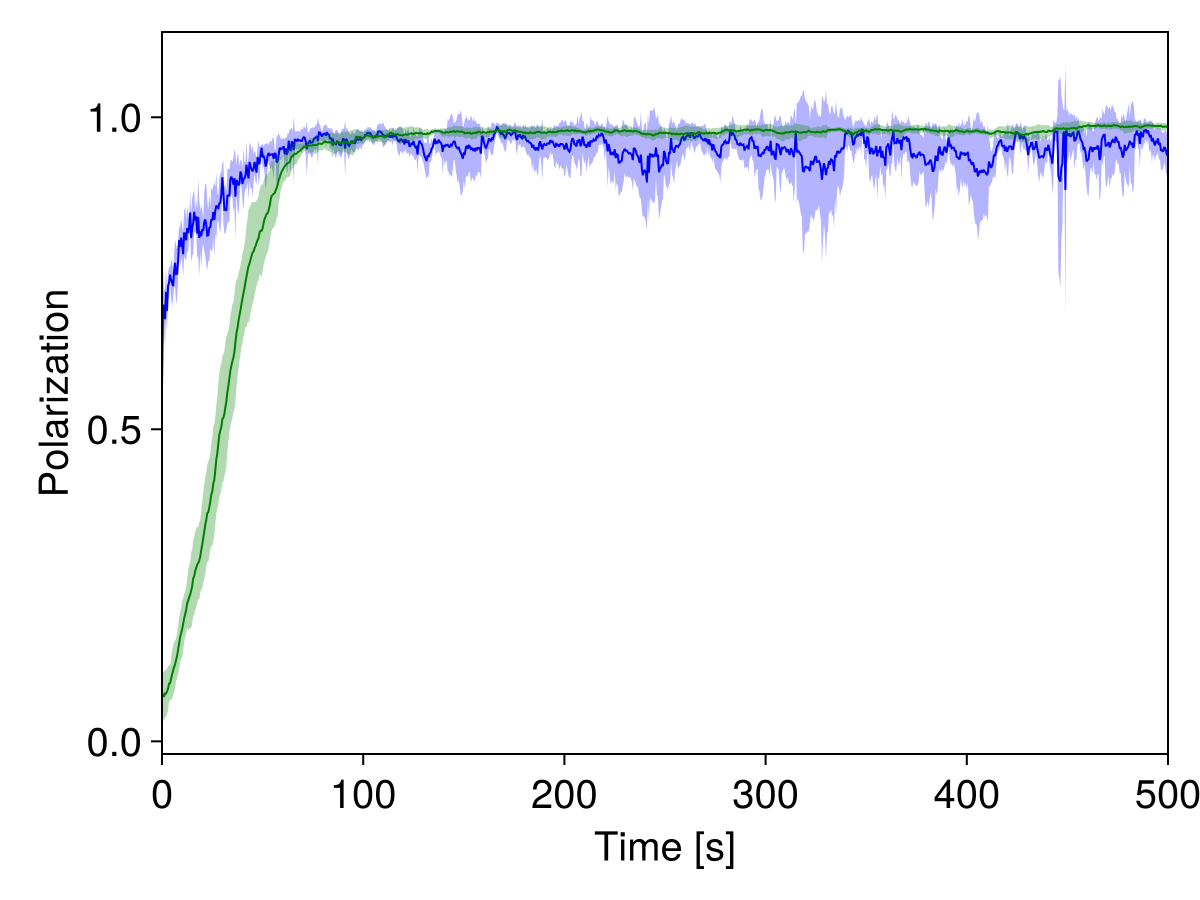
\includegraphics[width=.9\textwidth]{lj_vdist/polar1.0.png}}\\
			\subfloat[][]{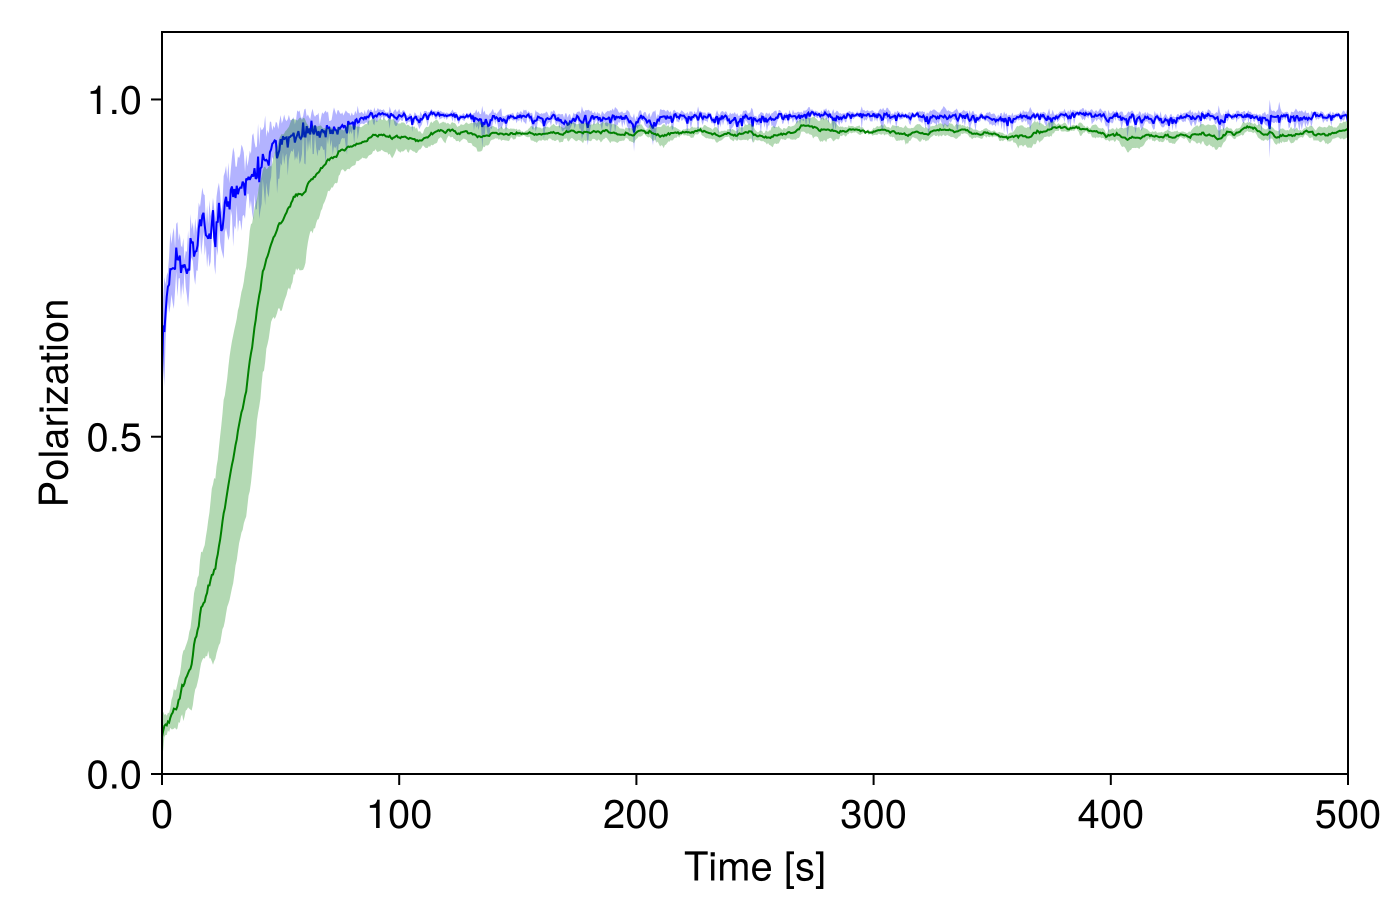
\includegraphics[width=.9\textwidth]{lj_vdist/polar2.0.png}}\\
			\subfloat[][]{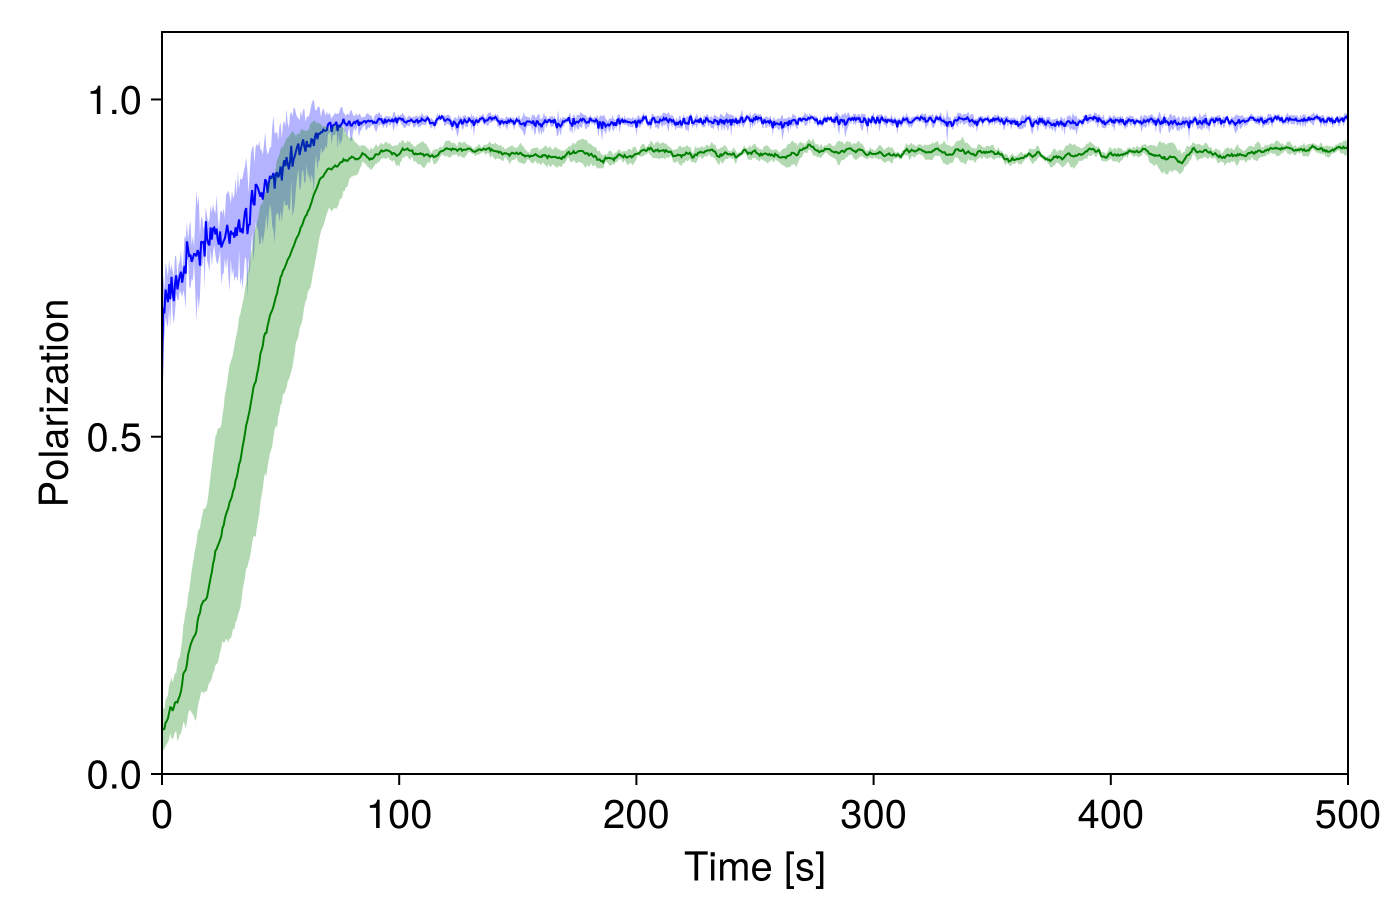
\includegraphics[width=.9\textwidth]{lj_vdist/polar5.0.png}}
			%\captionsetup{list=false}
			\caption[]{}
		\end{figure}
		\begin{figure}
			\centering
			\ContinuedFloat
			\subfloat[][]{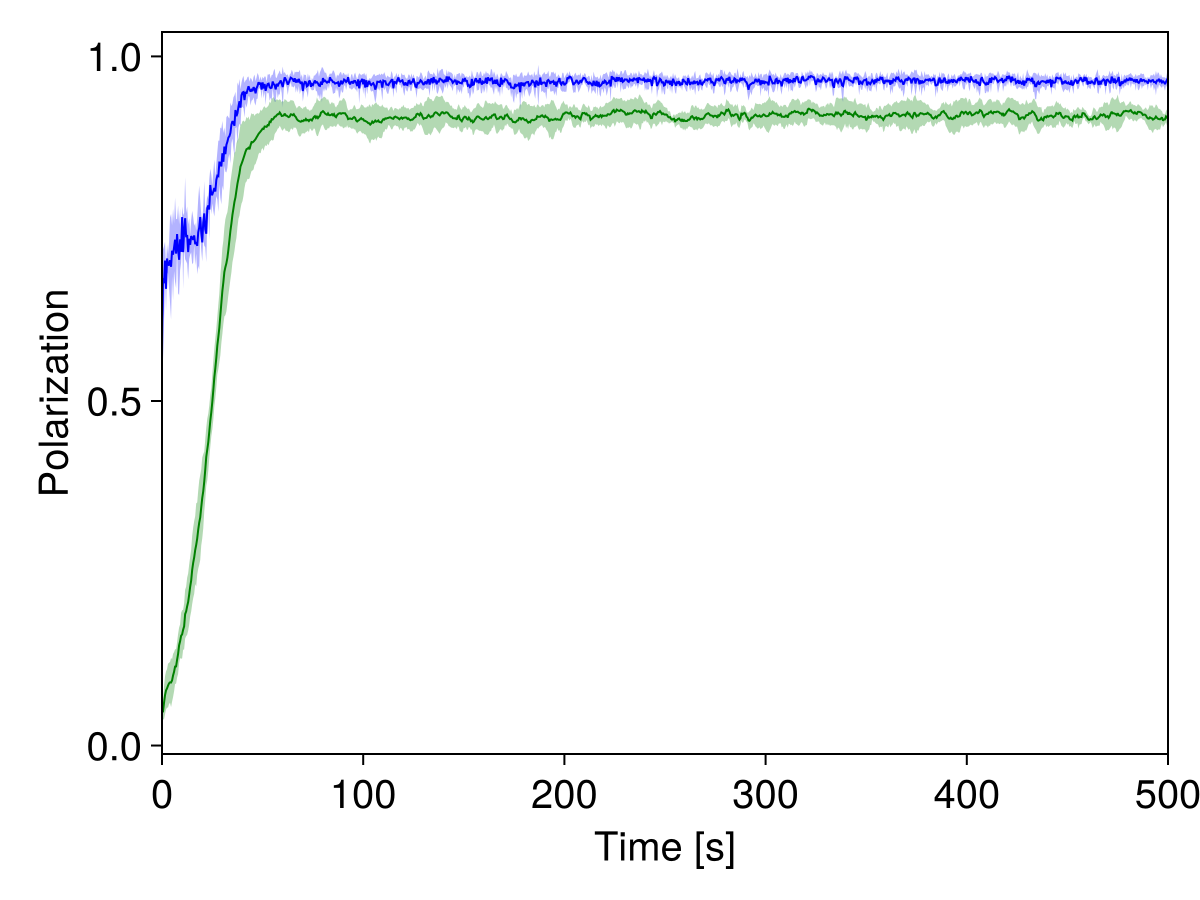
\includegraphics[width=.9\textwidth]{lj_vdist/polar10.0.png}}\\
			
			\caption{(continued) Local (blue) and global (green) polarization for a normal velocity distribution with $\mu = \SI{10}{\um\per\second}$ and standard deviation: (a) $\sigma = \SI{1}{\um\per\second}$, (b) $\sigma = \SI{2}{\um\per\second}$, (c) $\sigma = \SI{5}{\um\per\second}$, (d) $\sigma = \SI{10}{\um\per\second}$}
			\label{fig:lj_vdist_pol}
		\end{figure}
		
		\begin{figure}[hbtp]
			\centering\
			\subfloat[][]{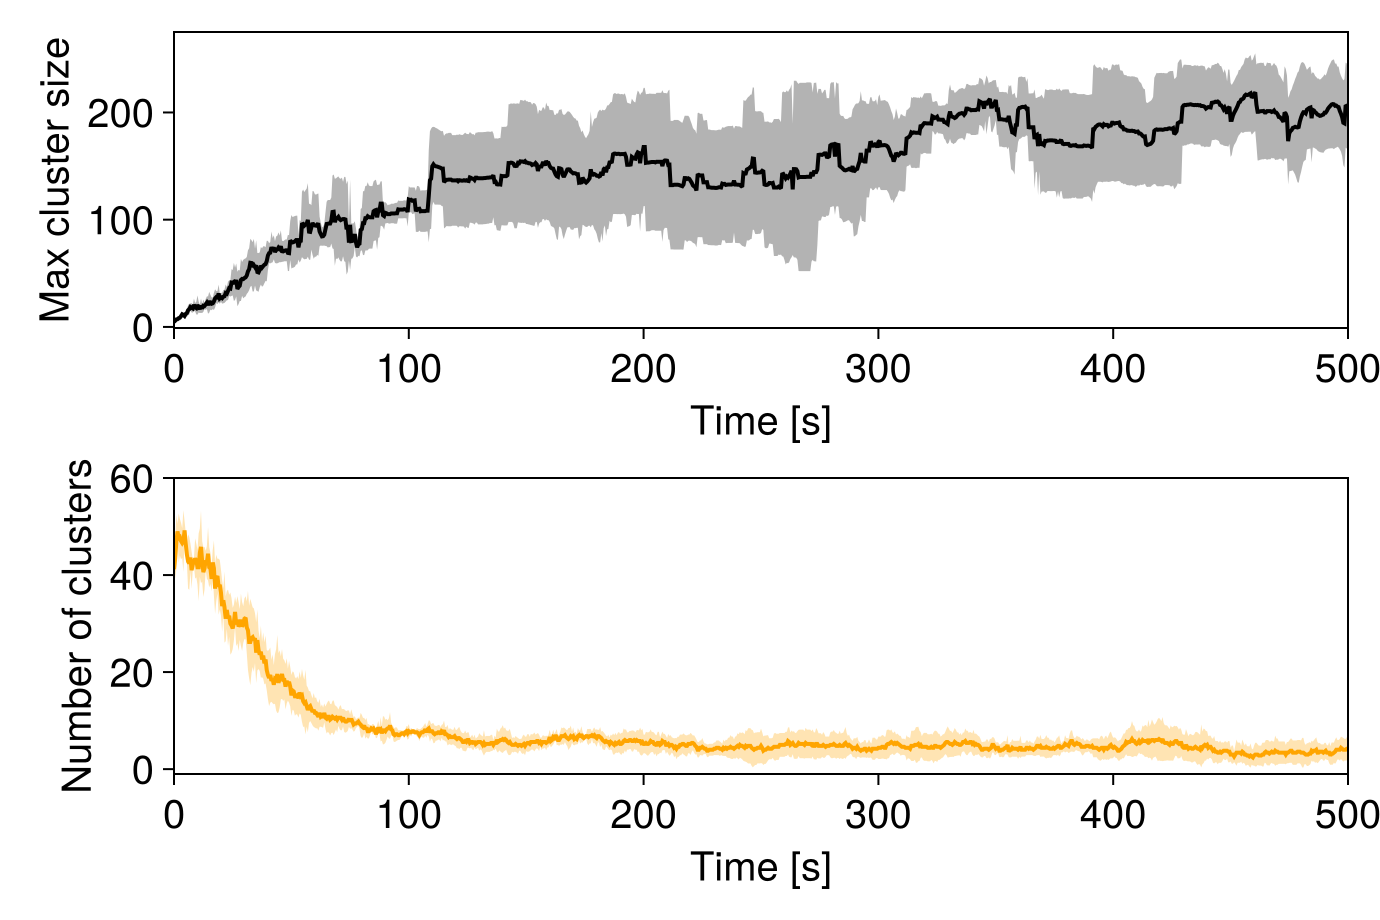
\includegraphics[width=.9\textwidth]{lj_vdist/cluster1.0.png}}\\
			\subfloat[][]{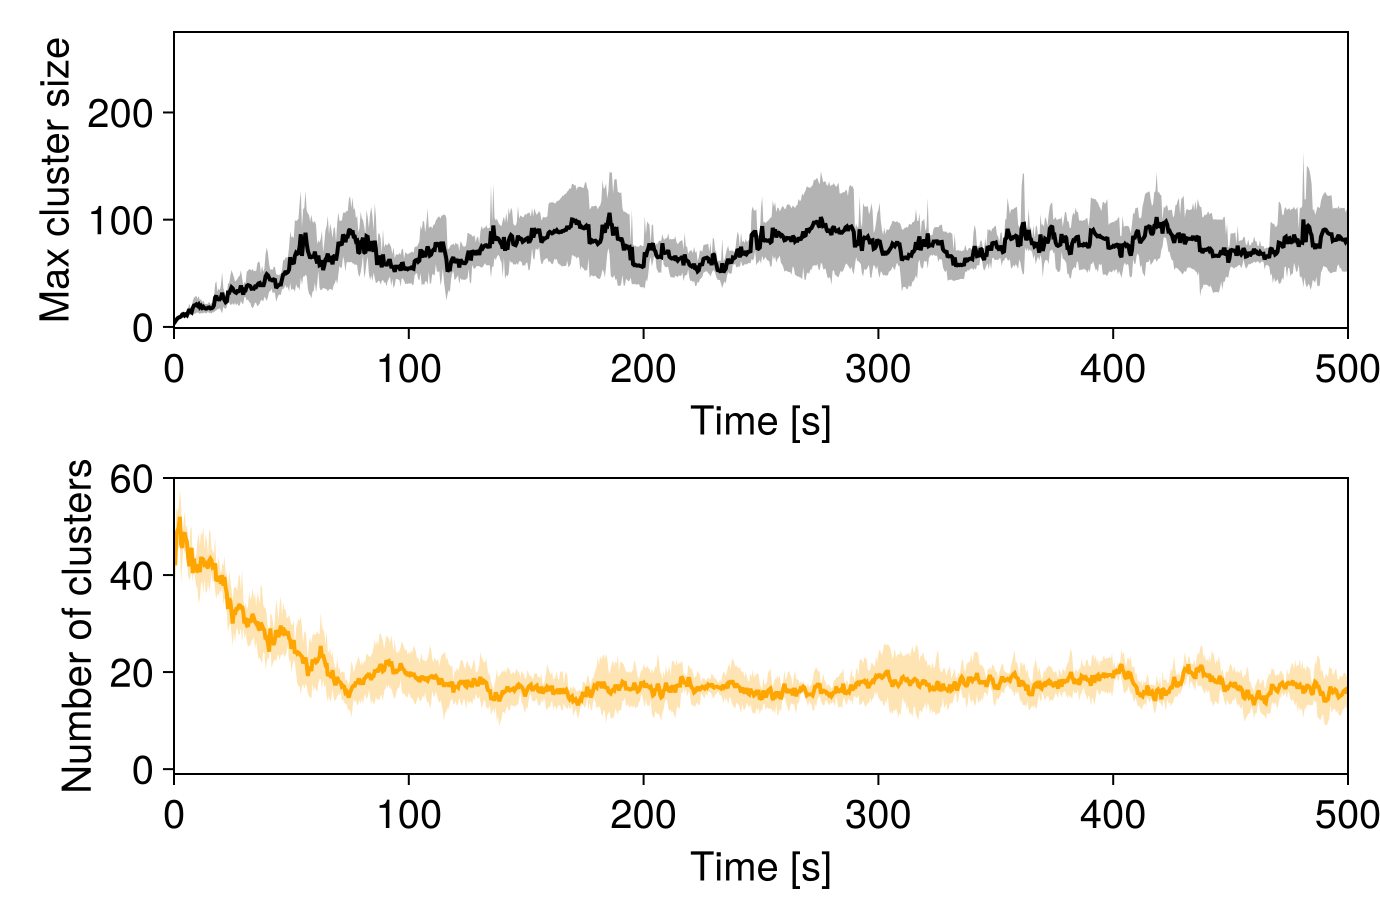
\includegraphics[width=.9\textwidth]{lj_vdist/cluster2.0.png}}\\
			\subfloat[][]{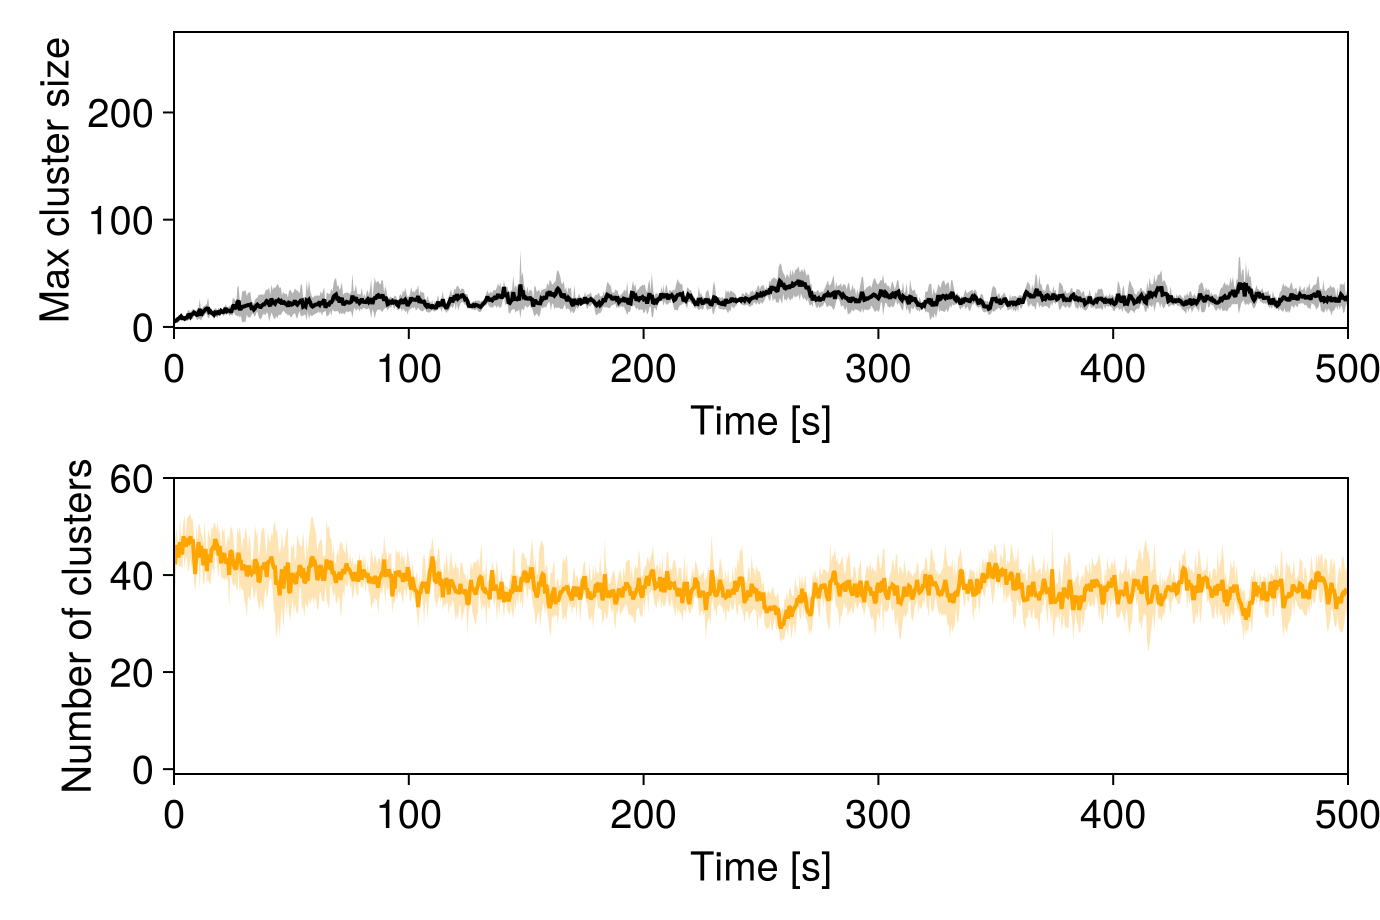
\includegraphics[width=.9\textwidth]{lj_vdist/cluster5.0.png}}
			%\captionsetup{list=false}
			\caption[]{}
		\end{figure}
		\begin{figure}[t]
			\centering
			\ContinuedFloat
			\subfloat[][]{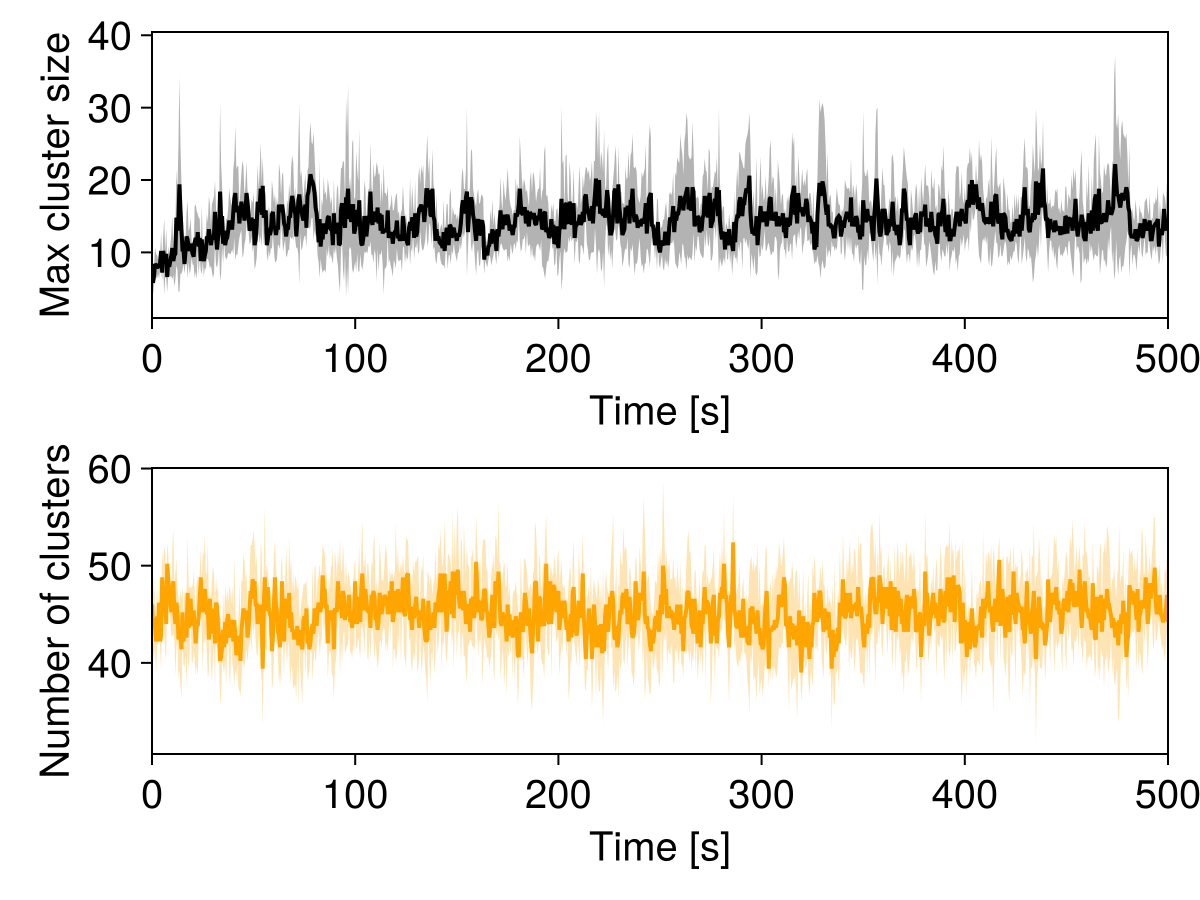
\includegraphics[width=.9\textwidth]{lj_vdist/cluster10.0.png}}\\
			
			\caption{(continued) Maximum cluster size and number of clusters for a normal velocity distribution with $\mu = \SI{10}{\um\per\second}$ and standard deviation: (a) $\sigma = \SI{1}{\um\per\second}$, (b) $\sigma = \SI{2}{\um\per\second}$, (c) $\sigma = \SI{5}{\um\per\second}$, (d) $\sigma = \SI{10}{\um\per\second}$}
			\label{fig:lj_vdist_clust}
		\end{figure}
		
		
		\begin{figure}[hbtp]
			\centering\
			\subfloat[][]{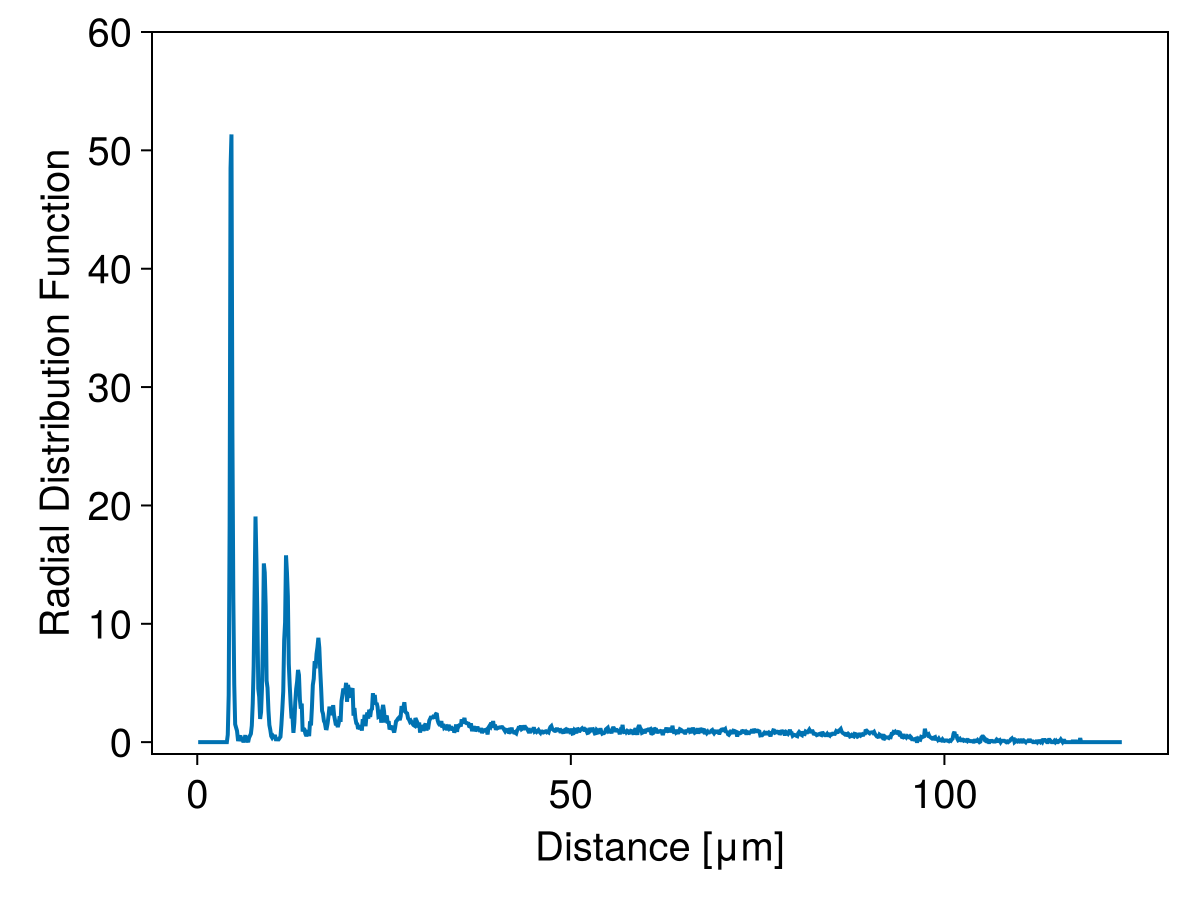
\includegraphics[width=.9\textwidth]{lj_vdist/rdf1.0.png}}\\
			\subfloat[][]{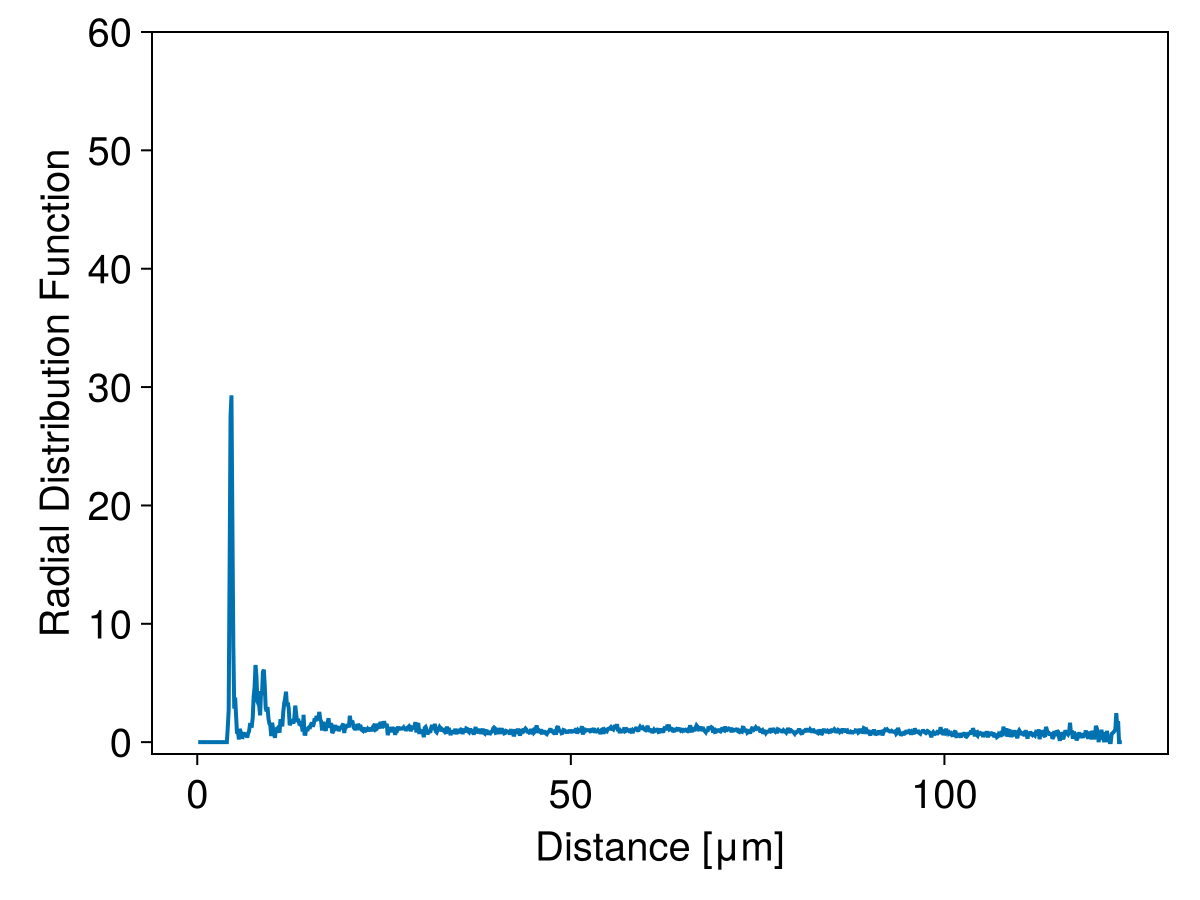
\includegraphics[width=.9\textwidth]{lj_vdist/rdf2.0.png}}\\
			\subfloat[][]{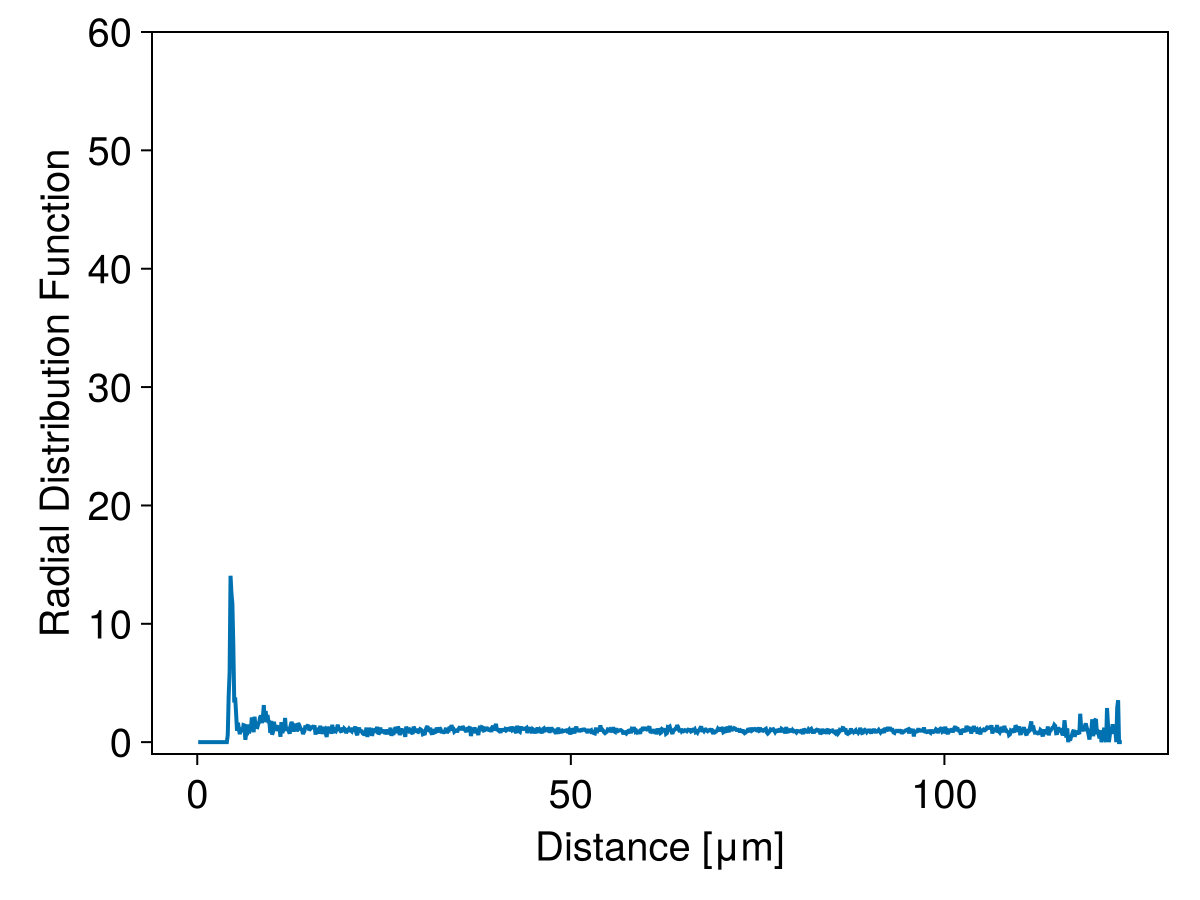
\includegraphics[width=.9\textwidth]{lj_vdist/rdf5.0.png}}
			%\captionsetup{list=false}
			\caption[]{}
		\end{figure}
		\begin{figure}
			\centering
			\ContinuedFloat
			\subfloat[][]{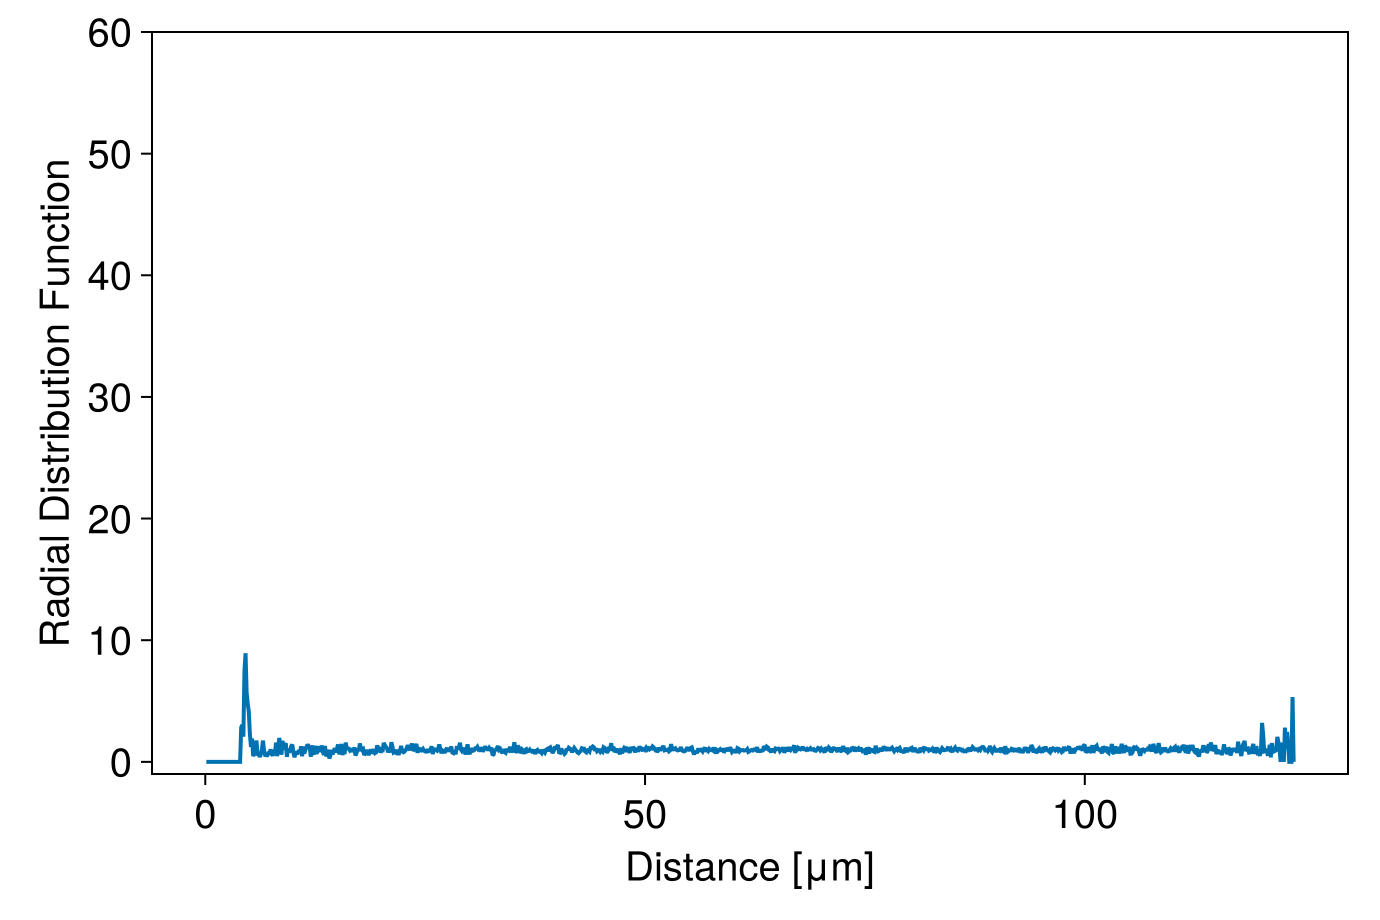
\includegraphics[width=.9\textwidth]{lj_vdist/rdf10.0.png}}\\
			
			\caption{Radial distribution function at last instant of simulation for a normal velocity distribution with $\mu = \SI{10}{\um\per\second}$ and standard deviation: (a) $\sigma = \SI{1}{\um\per\second}$, (b) $\sigma = \SI{2}{\um\per\second}$, (c) $\sigma = \SI{5}{\um\per\second}$, (d) $\sigma = \SI{10}{\um\per\second}$.}
			\label{fig:lj_vdist_rdf}
		\end{figure}
		
		\subsection{Orientation Coupling}%\todo{questa la metterei prima della sezione sulla distribuzione di velocità, così hai per primi i due parametri, e poi le distribuzioni}
		To understand the role of the orientational coupling parameter $\alpha$, we performed simulations with velocity \SI{20}{\um\per\second}, varying $\alpha$ between \numlist{-0.75; 0.75} in \num{0.25} increments. 
		Here, a  high positive coupling value with positive sign means making the interacting positions of two particles closer when they are moving towards each other in a head to head fashion.
		For this reason, when $\alpha = 0.75$, integration step is decreased to \SI{2.5e-4}{\second} to avoid instabilities due to the LJ nonlinearity.
		
		Results relative to zero coupling show how clustering and polarization are related in this case: not only the absence of an alignment interaction hinders system's polarization as expected, but at this level, large scale clustering does not realize although an attractive force is inserted in simulations.
		
		With $\alpha = 0.25$ system tends to polarize, both locally and globally, but still it does not cluster as a whole. 
		Some peaks at short distance start to rise in the $g(r)$ (Figure \ref{fig:lj_oc_rdf}), showing the onset of short range order, though they are not in the typical positions of a hexagonal close packed lattice.
		%\todo{anche qui la numerazione fa casino a causa della figura spezzata}
		
		At $\alpha = 0.5$ polarization is almost total and all particles in the system tend to be part of the same cluster.
		Radial distribution function shows the onset of long range order, with high and narrow peaks, both at short and long distance.
		
		Polarization is total at $\alpha = 0.75$, and once steady state is reached, both local and global alignment present very small oscillations.
		Ensemble is fully clustered and flocking at this point.
		
		Analyzing the transient time, it is possible to notice how increasing the coupling parameter between orientation angles tends to reduce the transient time, making it faster for the system to align (Figure \ref{fig:transienttime_oc}).
		\begin{figure}[htp]
			\centering
			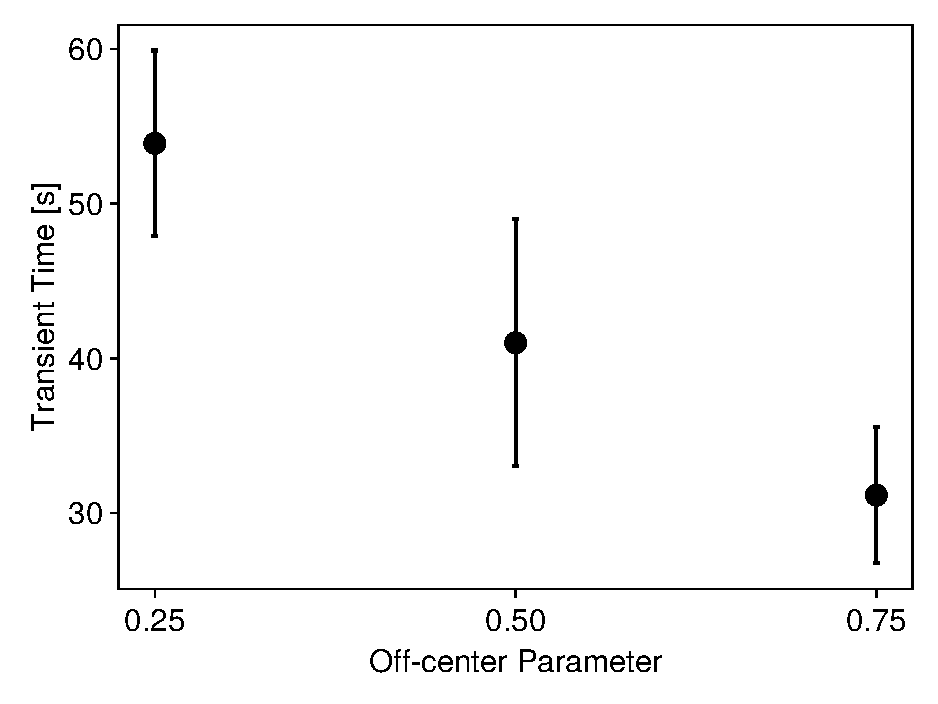
\includegraphics[width = \singfigwidth]{lj_oc/transient_time_alpha.pdf}
			
			\caption{Transient time (time needed to reach 95\% of maximum) for global polarization as a function of $\alpha$. Only positive values of off center coupling (where the system polarizes) are showed here.}
			\label{fig:transienttime_oc}
		\end{figure}
		
		All of the three simulations with negative $\alpha$ show no alignment and no clustering, in accordance with what stated in section \ref{velocity}.
		
		\begin{figure}[hbtp]
			\centering\
			\subfloat[][]{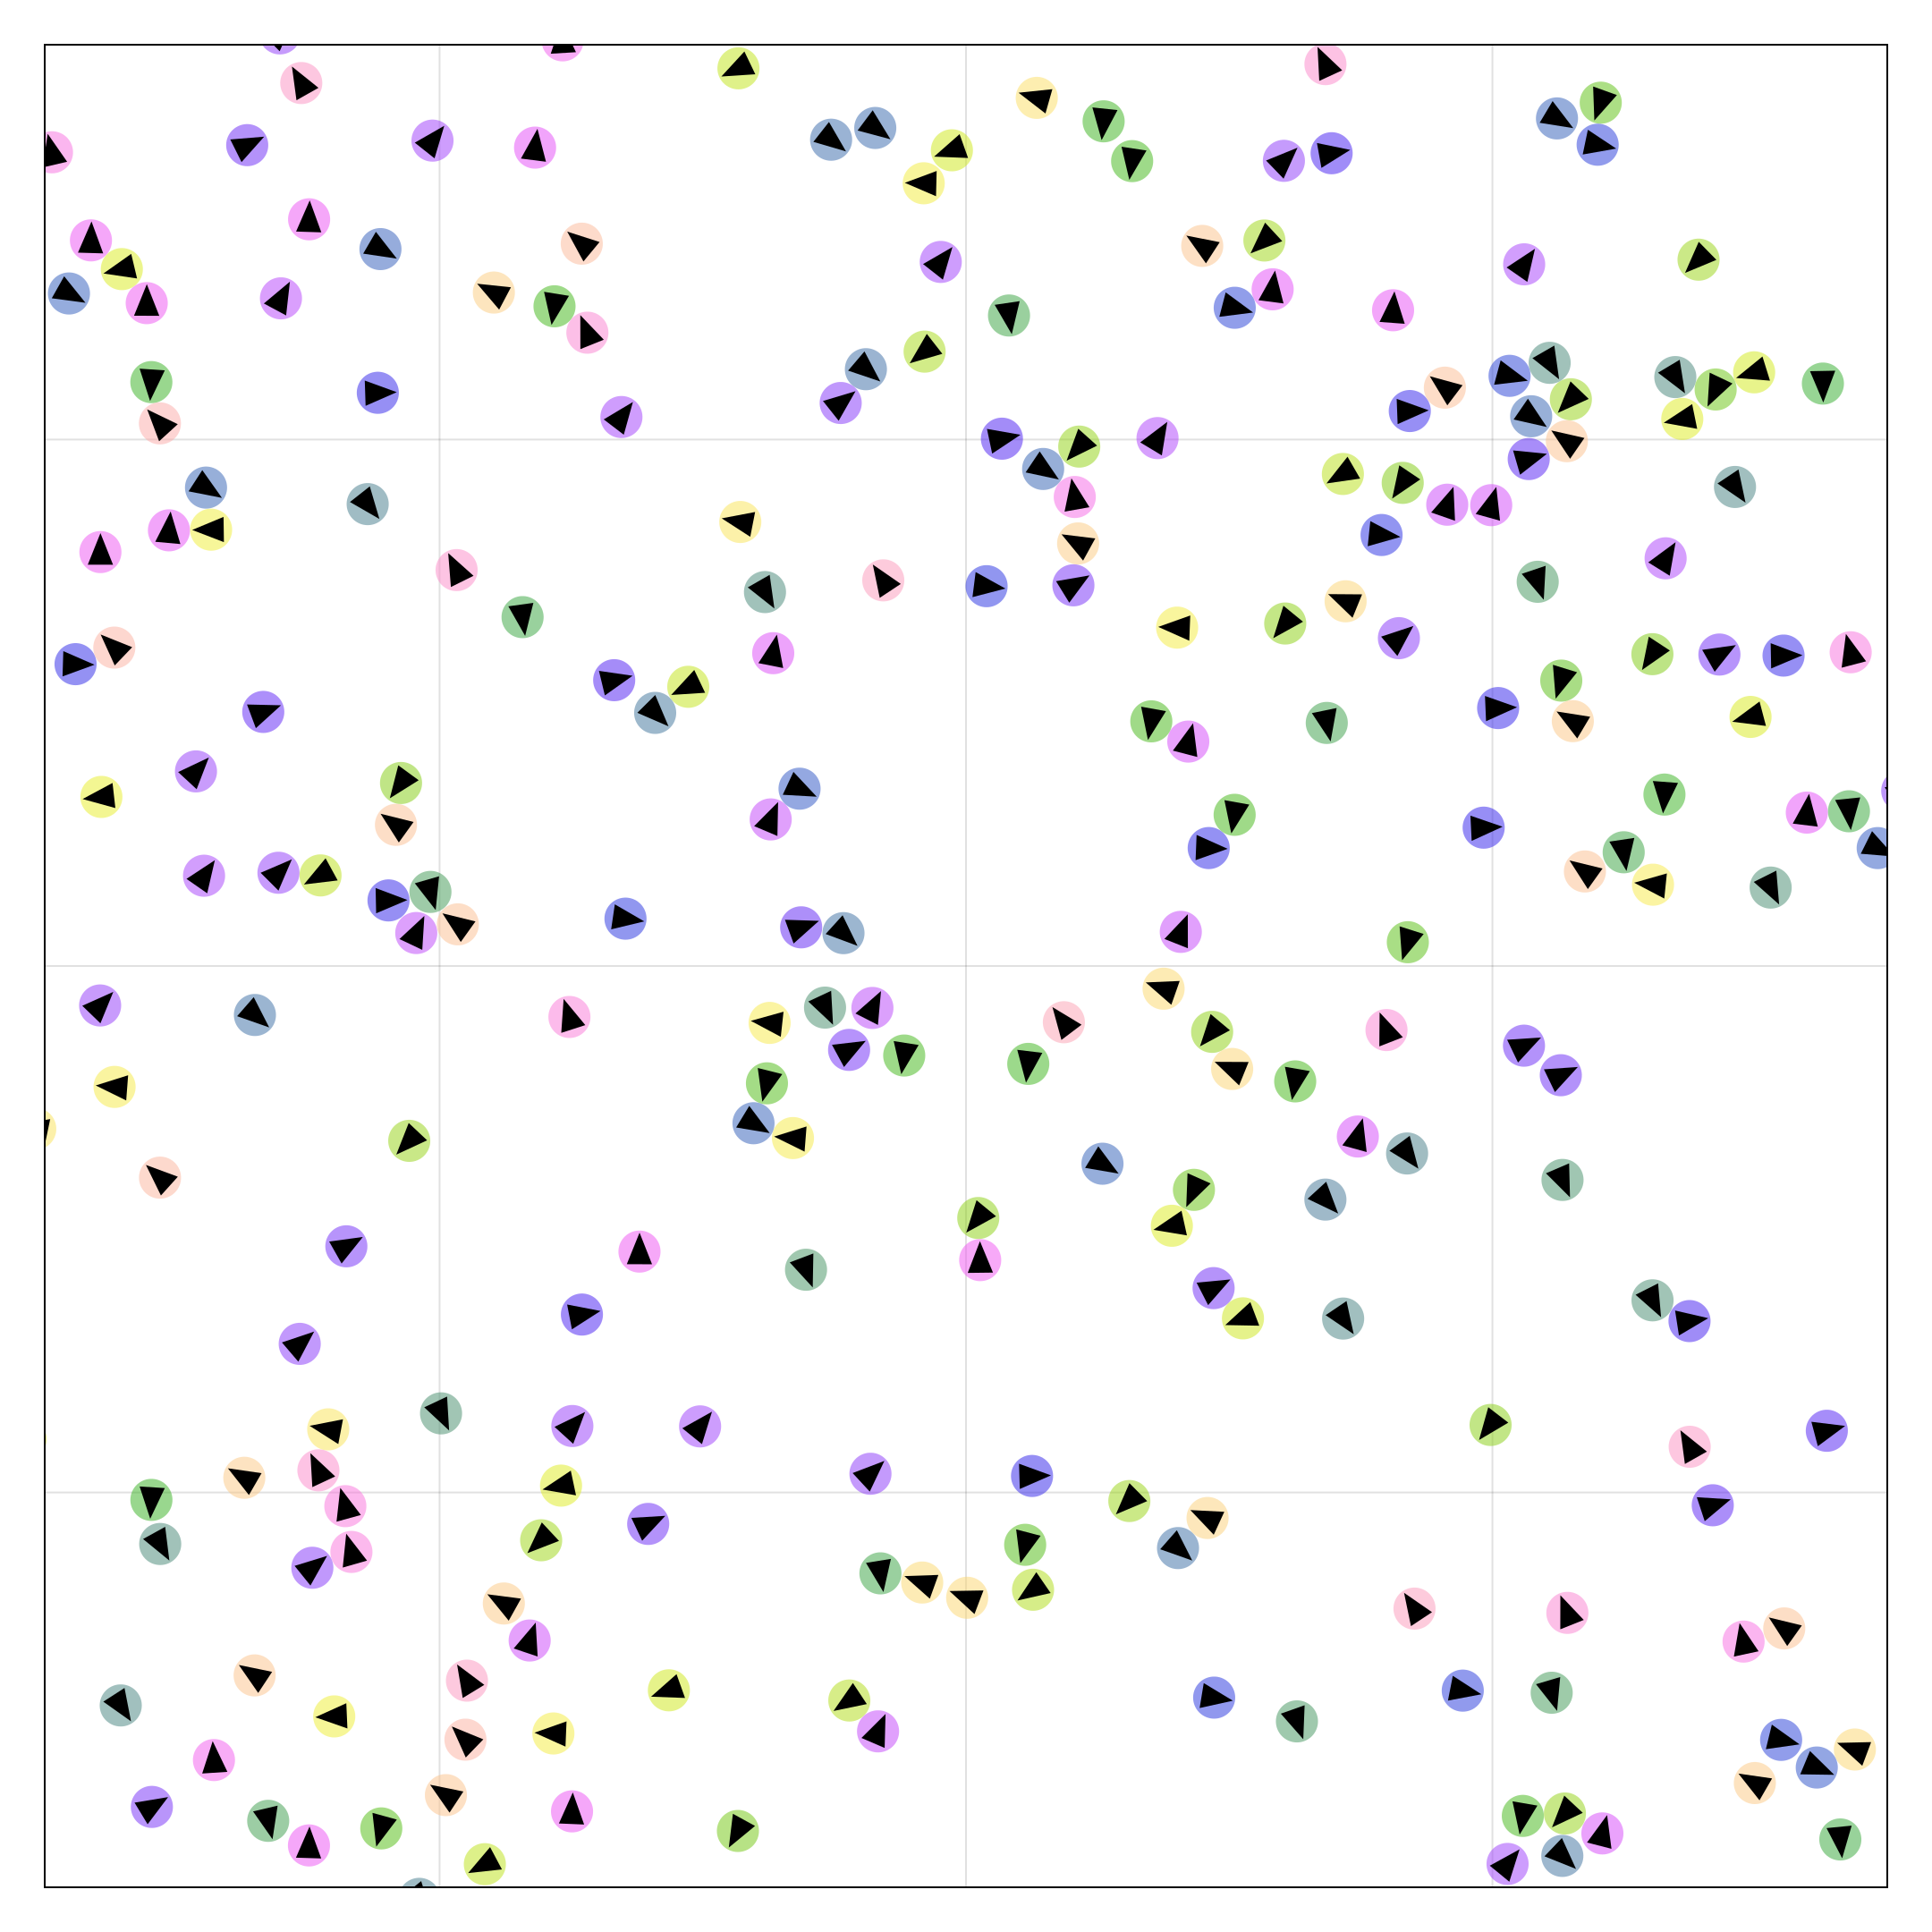
\includegraphics[width=.5\textwidth]{lj_oc/situa-0.75.png}}
			\subfloat[][]{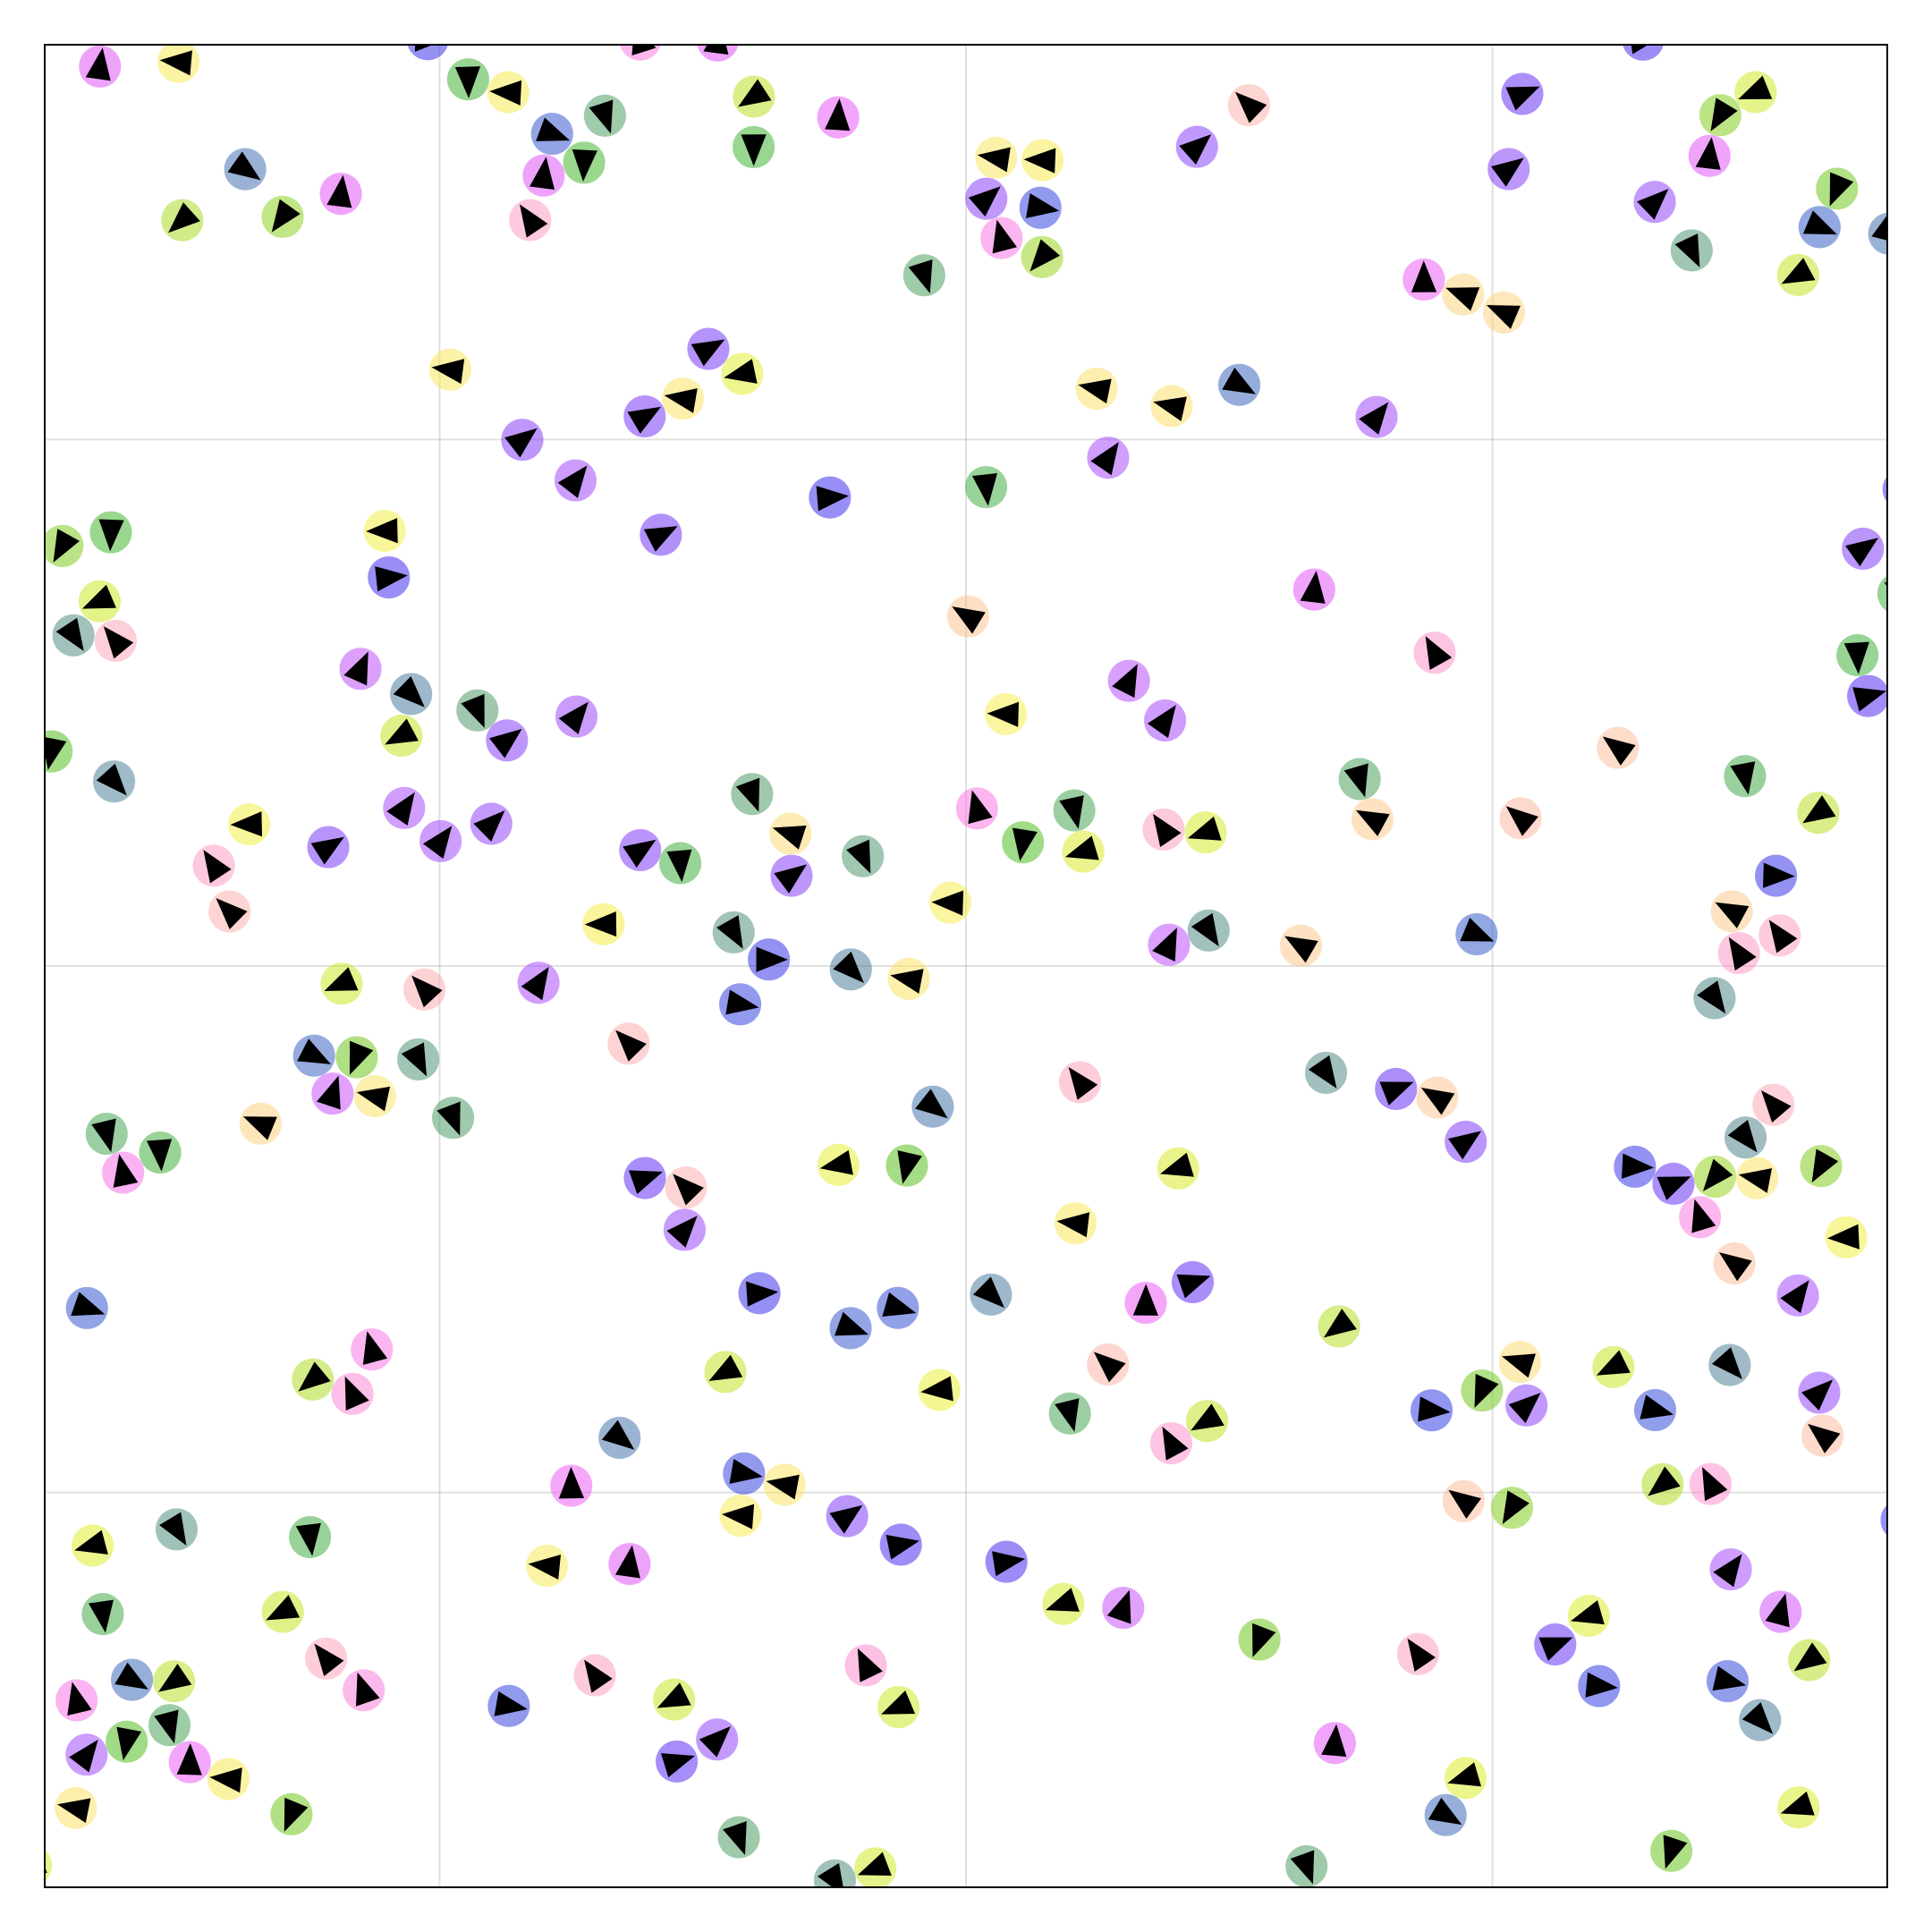
\includegraphics[width=.5\textwidth]{lj_oc/situa-0.5.png}}\\
			\subfloat[][]{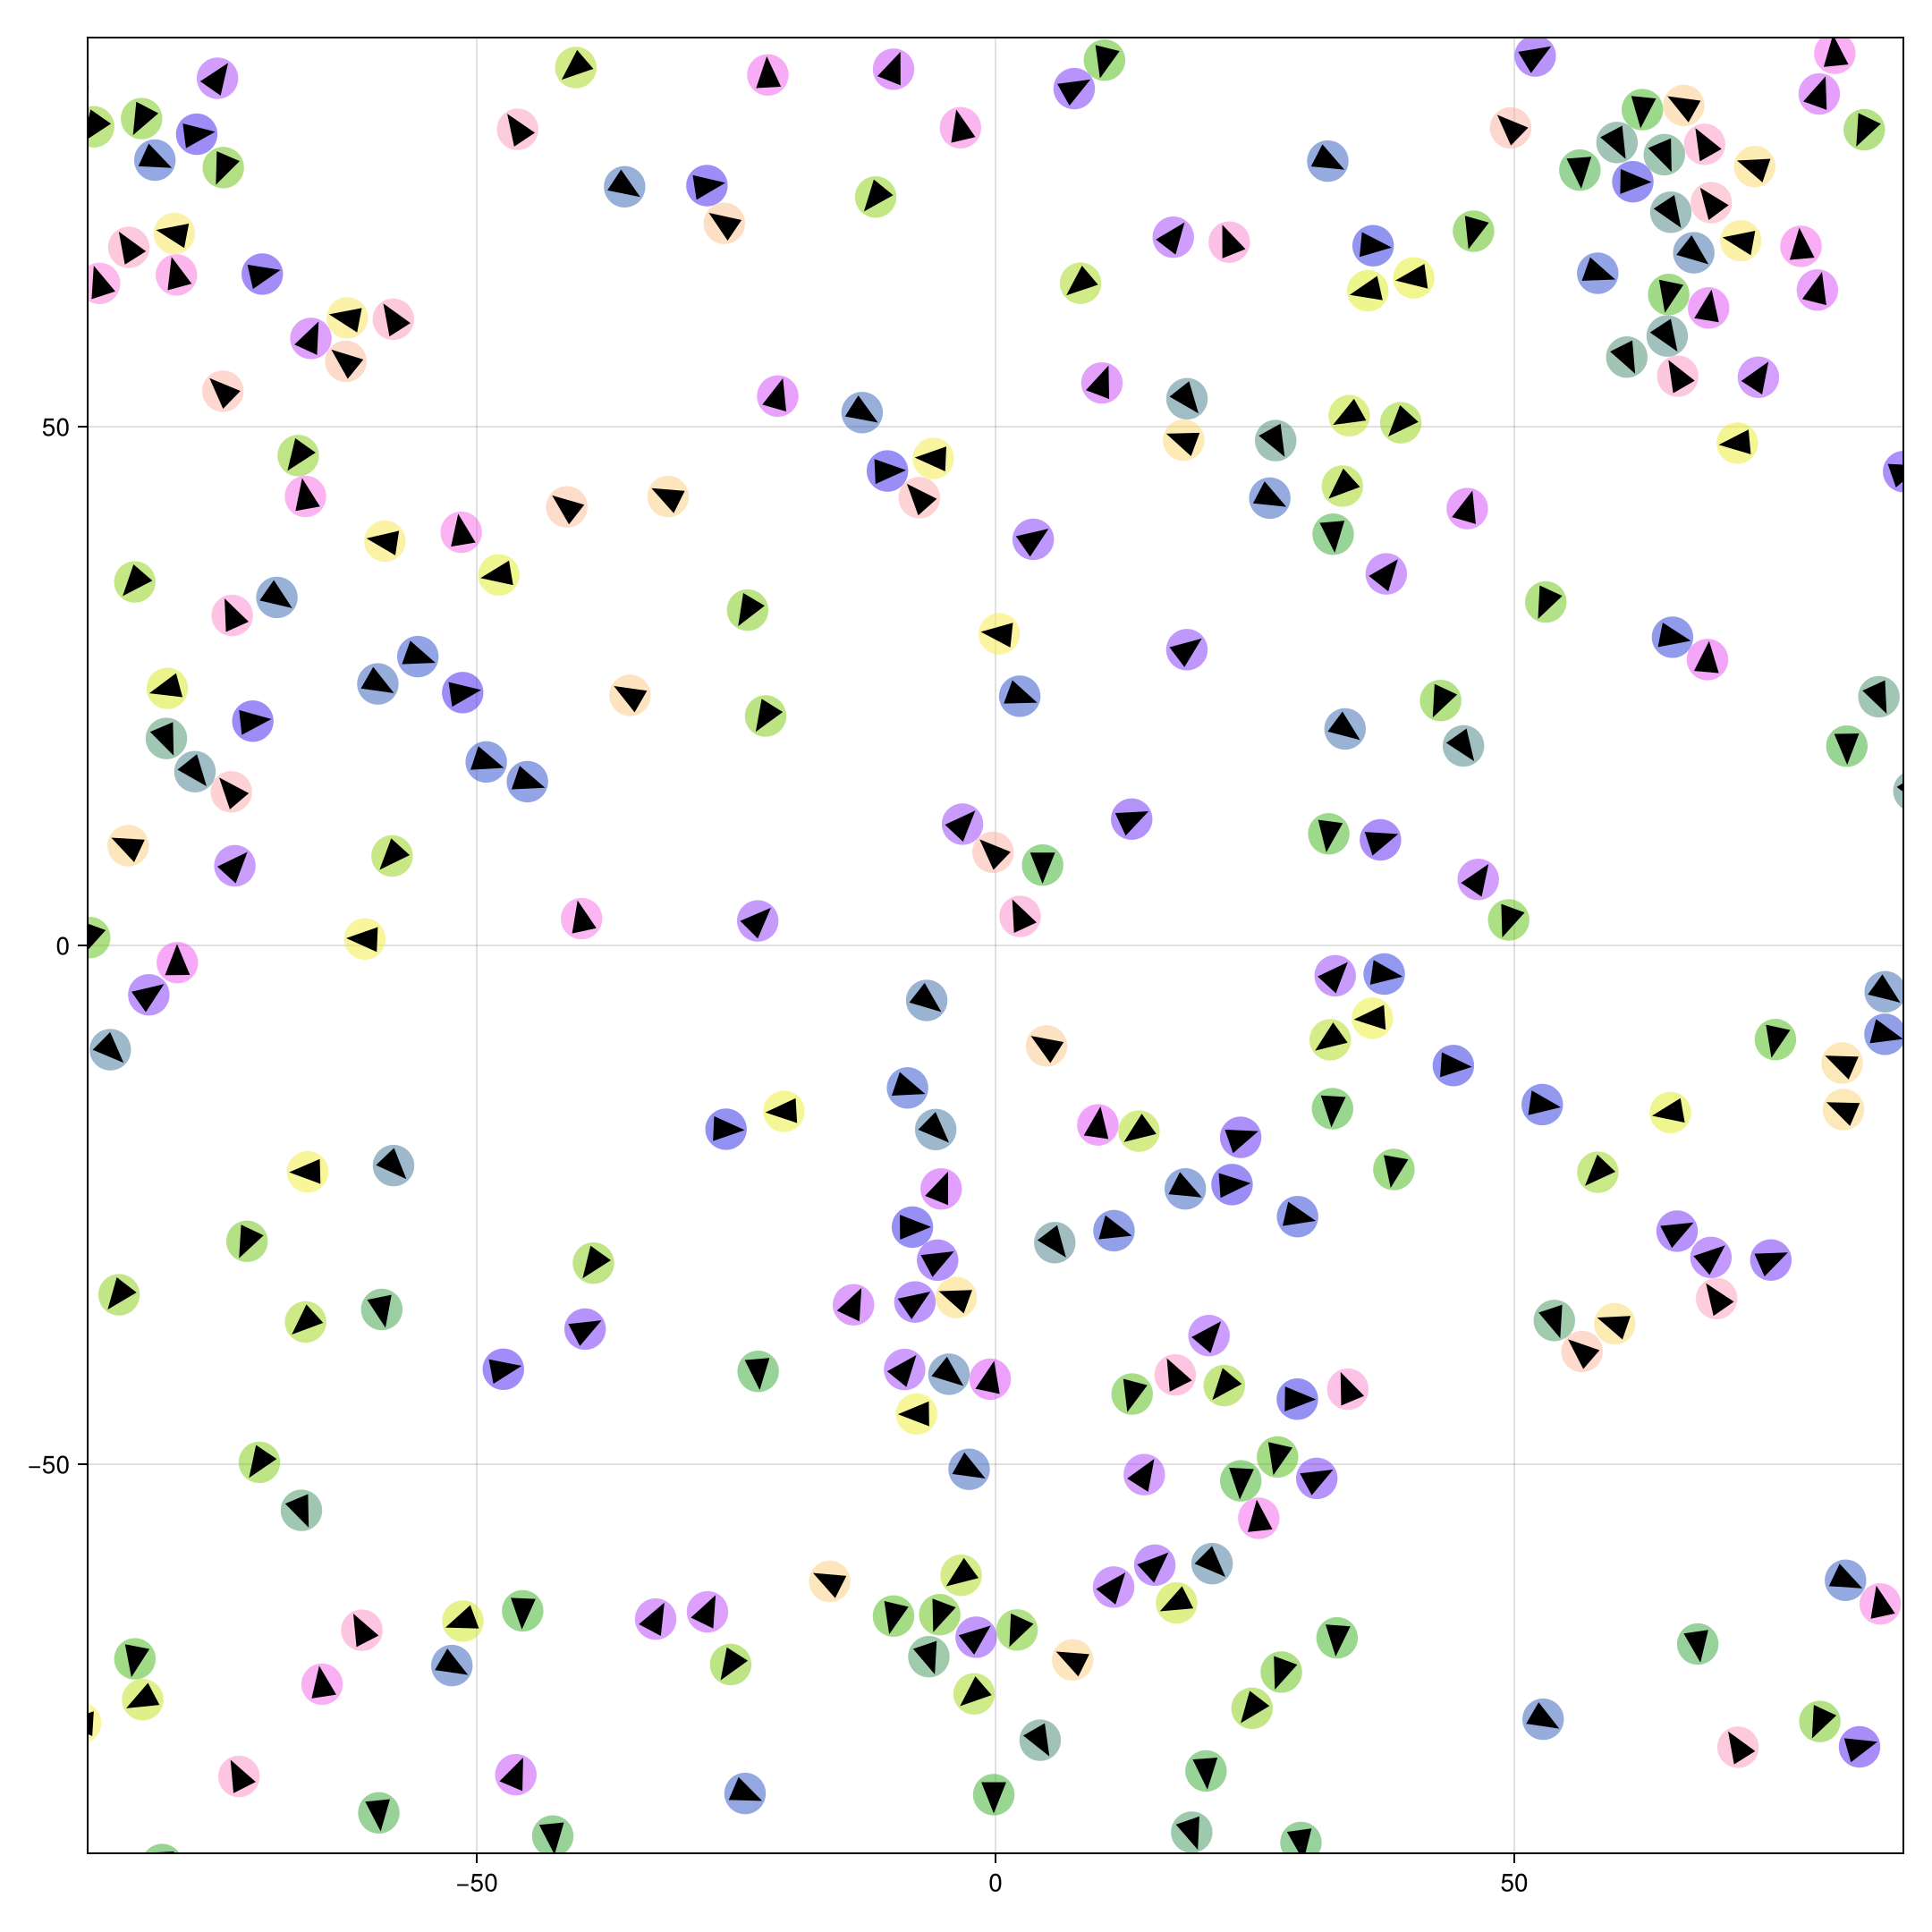
\includegraphics[width=.5\textwidth]{lj_oc/situa-0.25.png}}
			\subfloat[][]{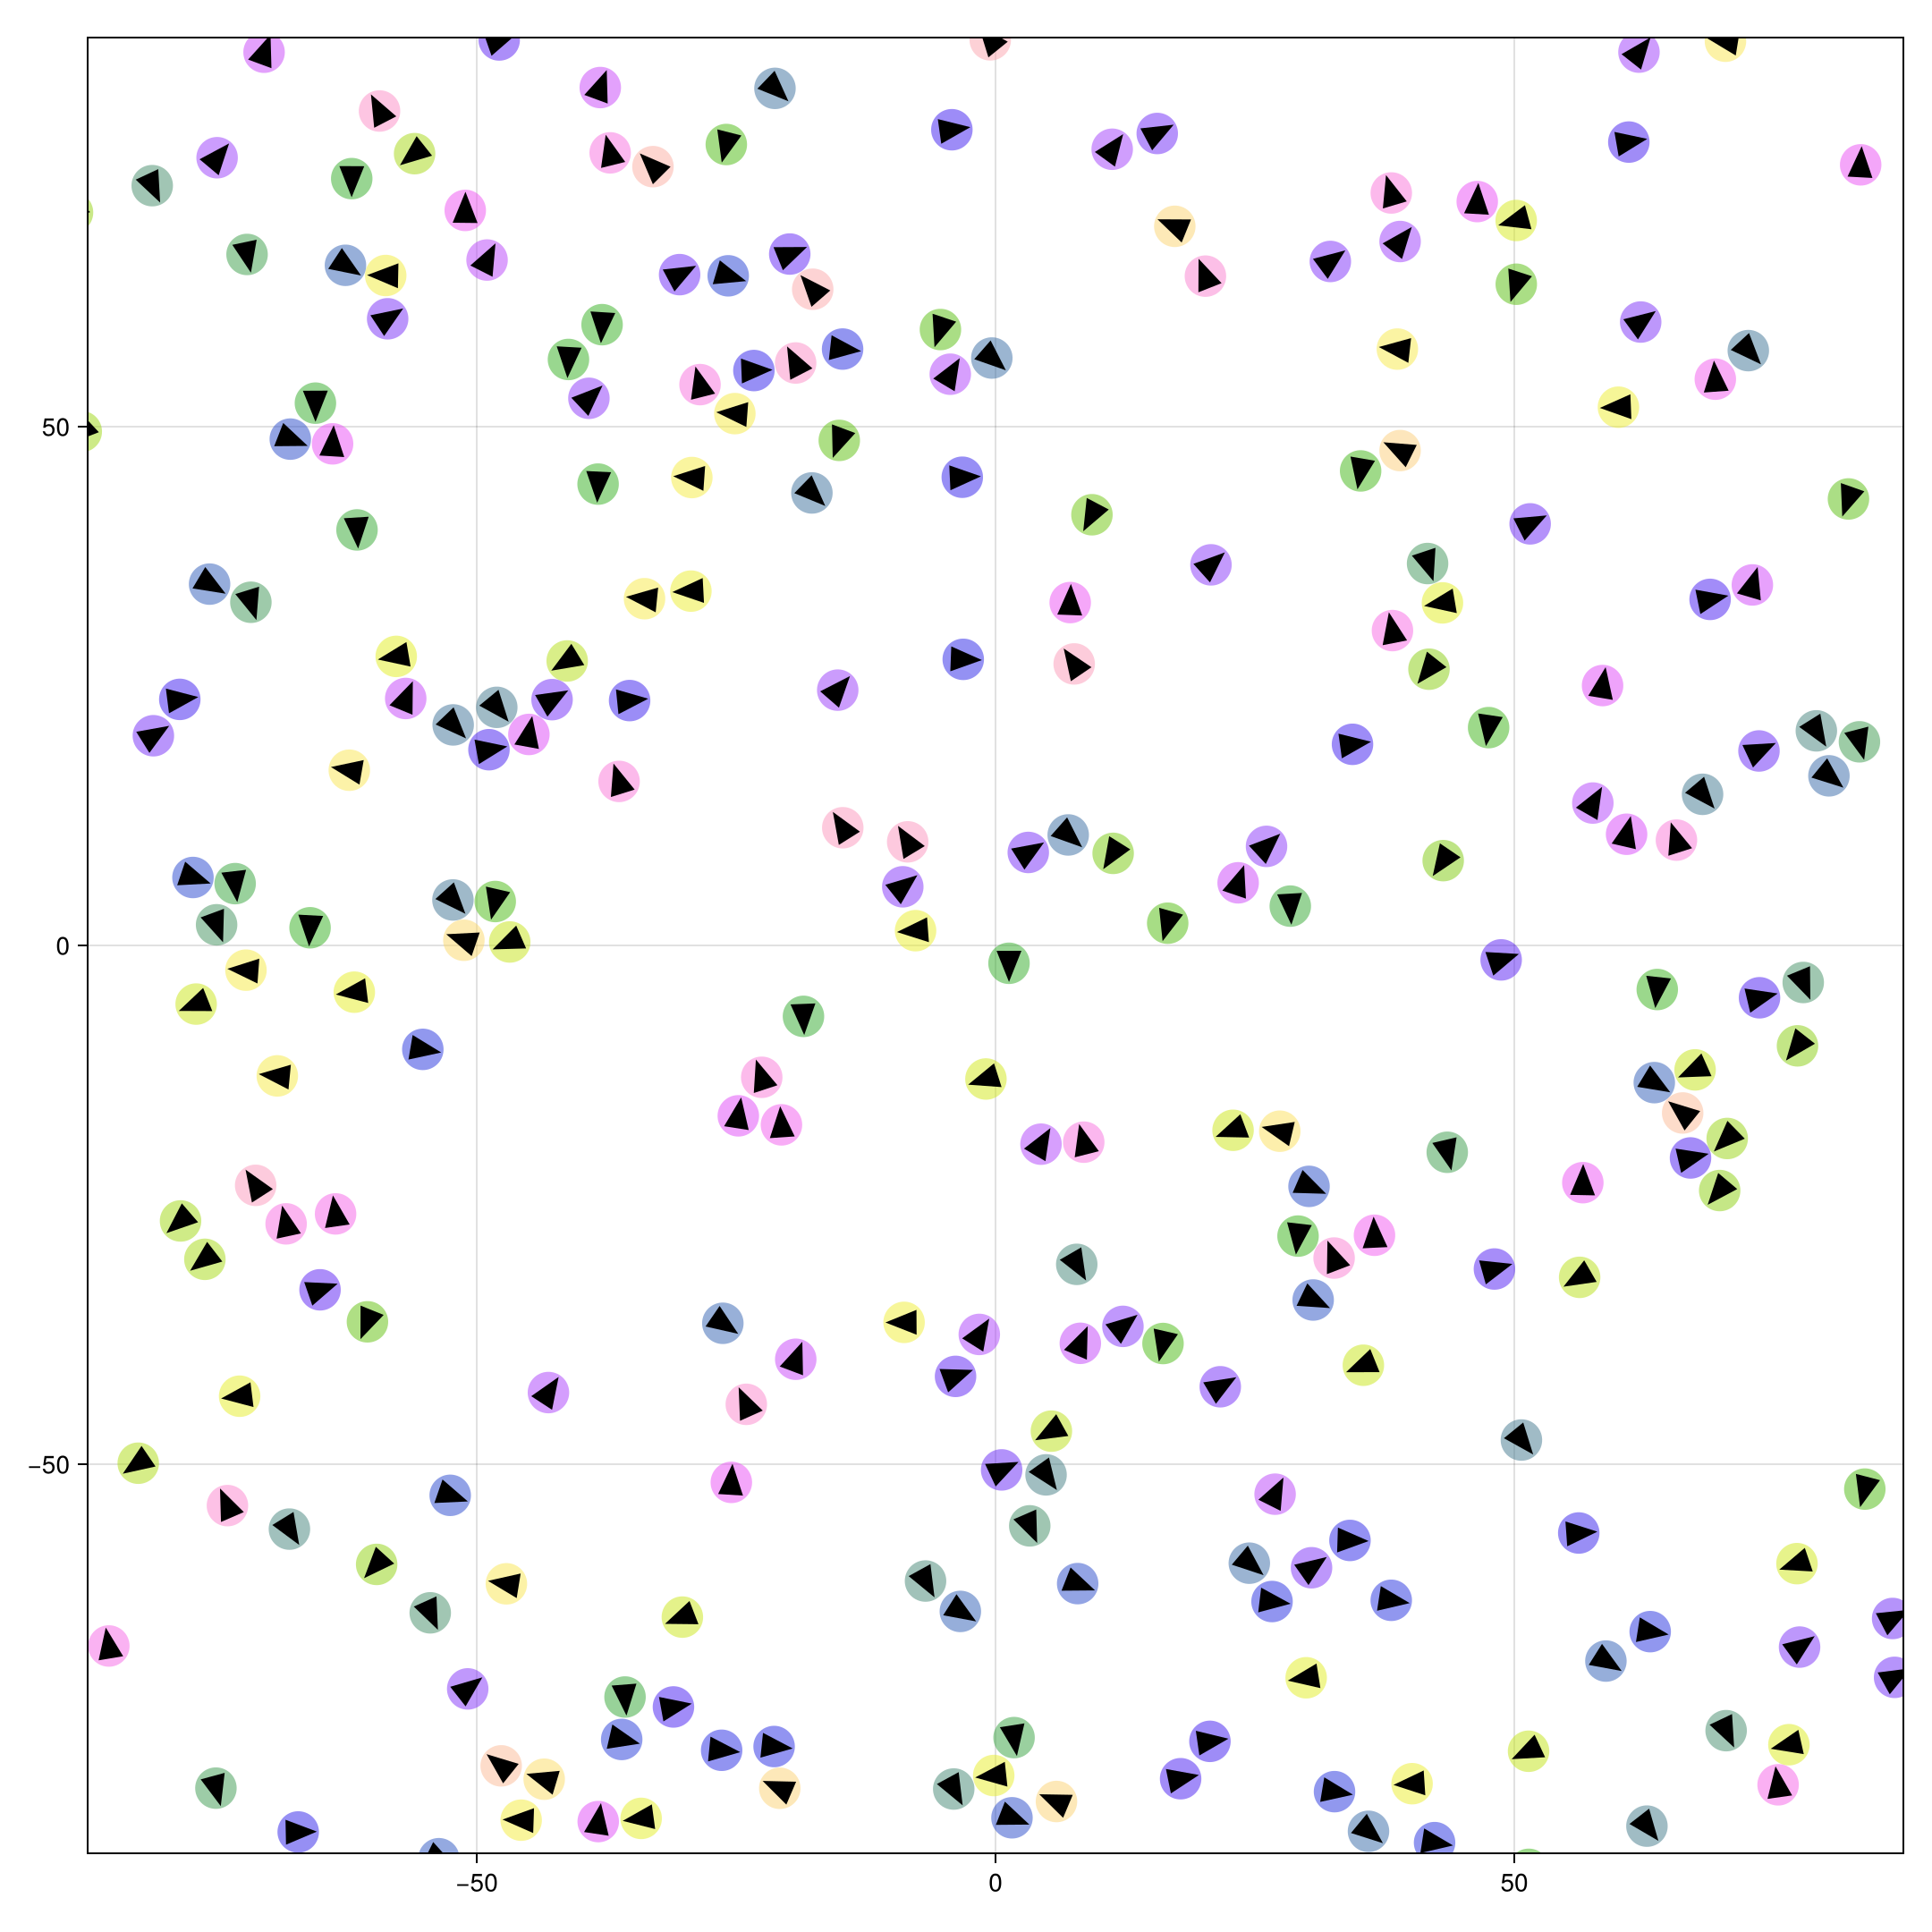
\includegraphics[width=.5\textwidth]{lj_oc/situa0.0.png}}\\
			\subfloat[][]{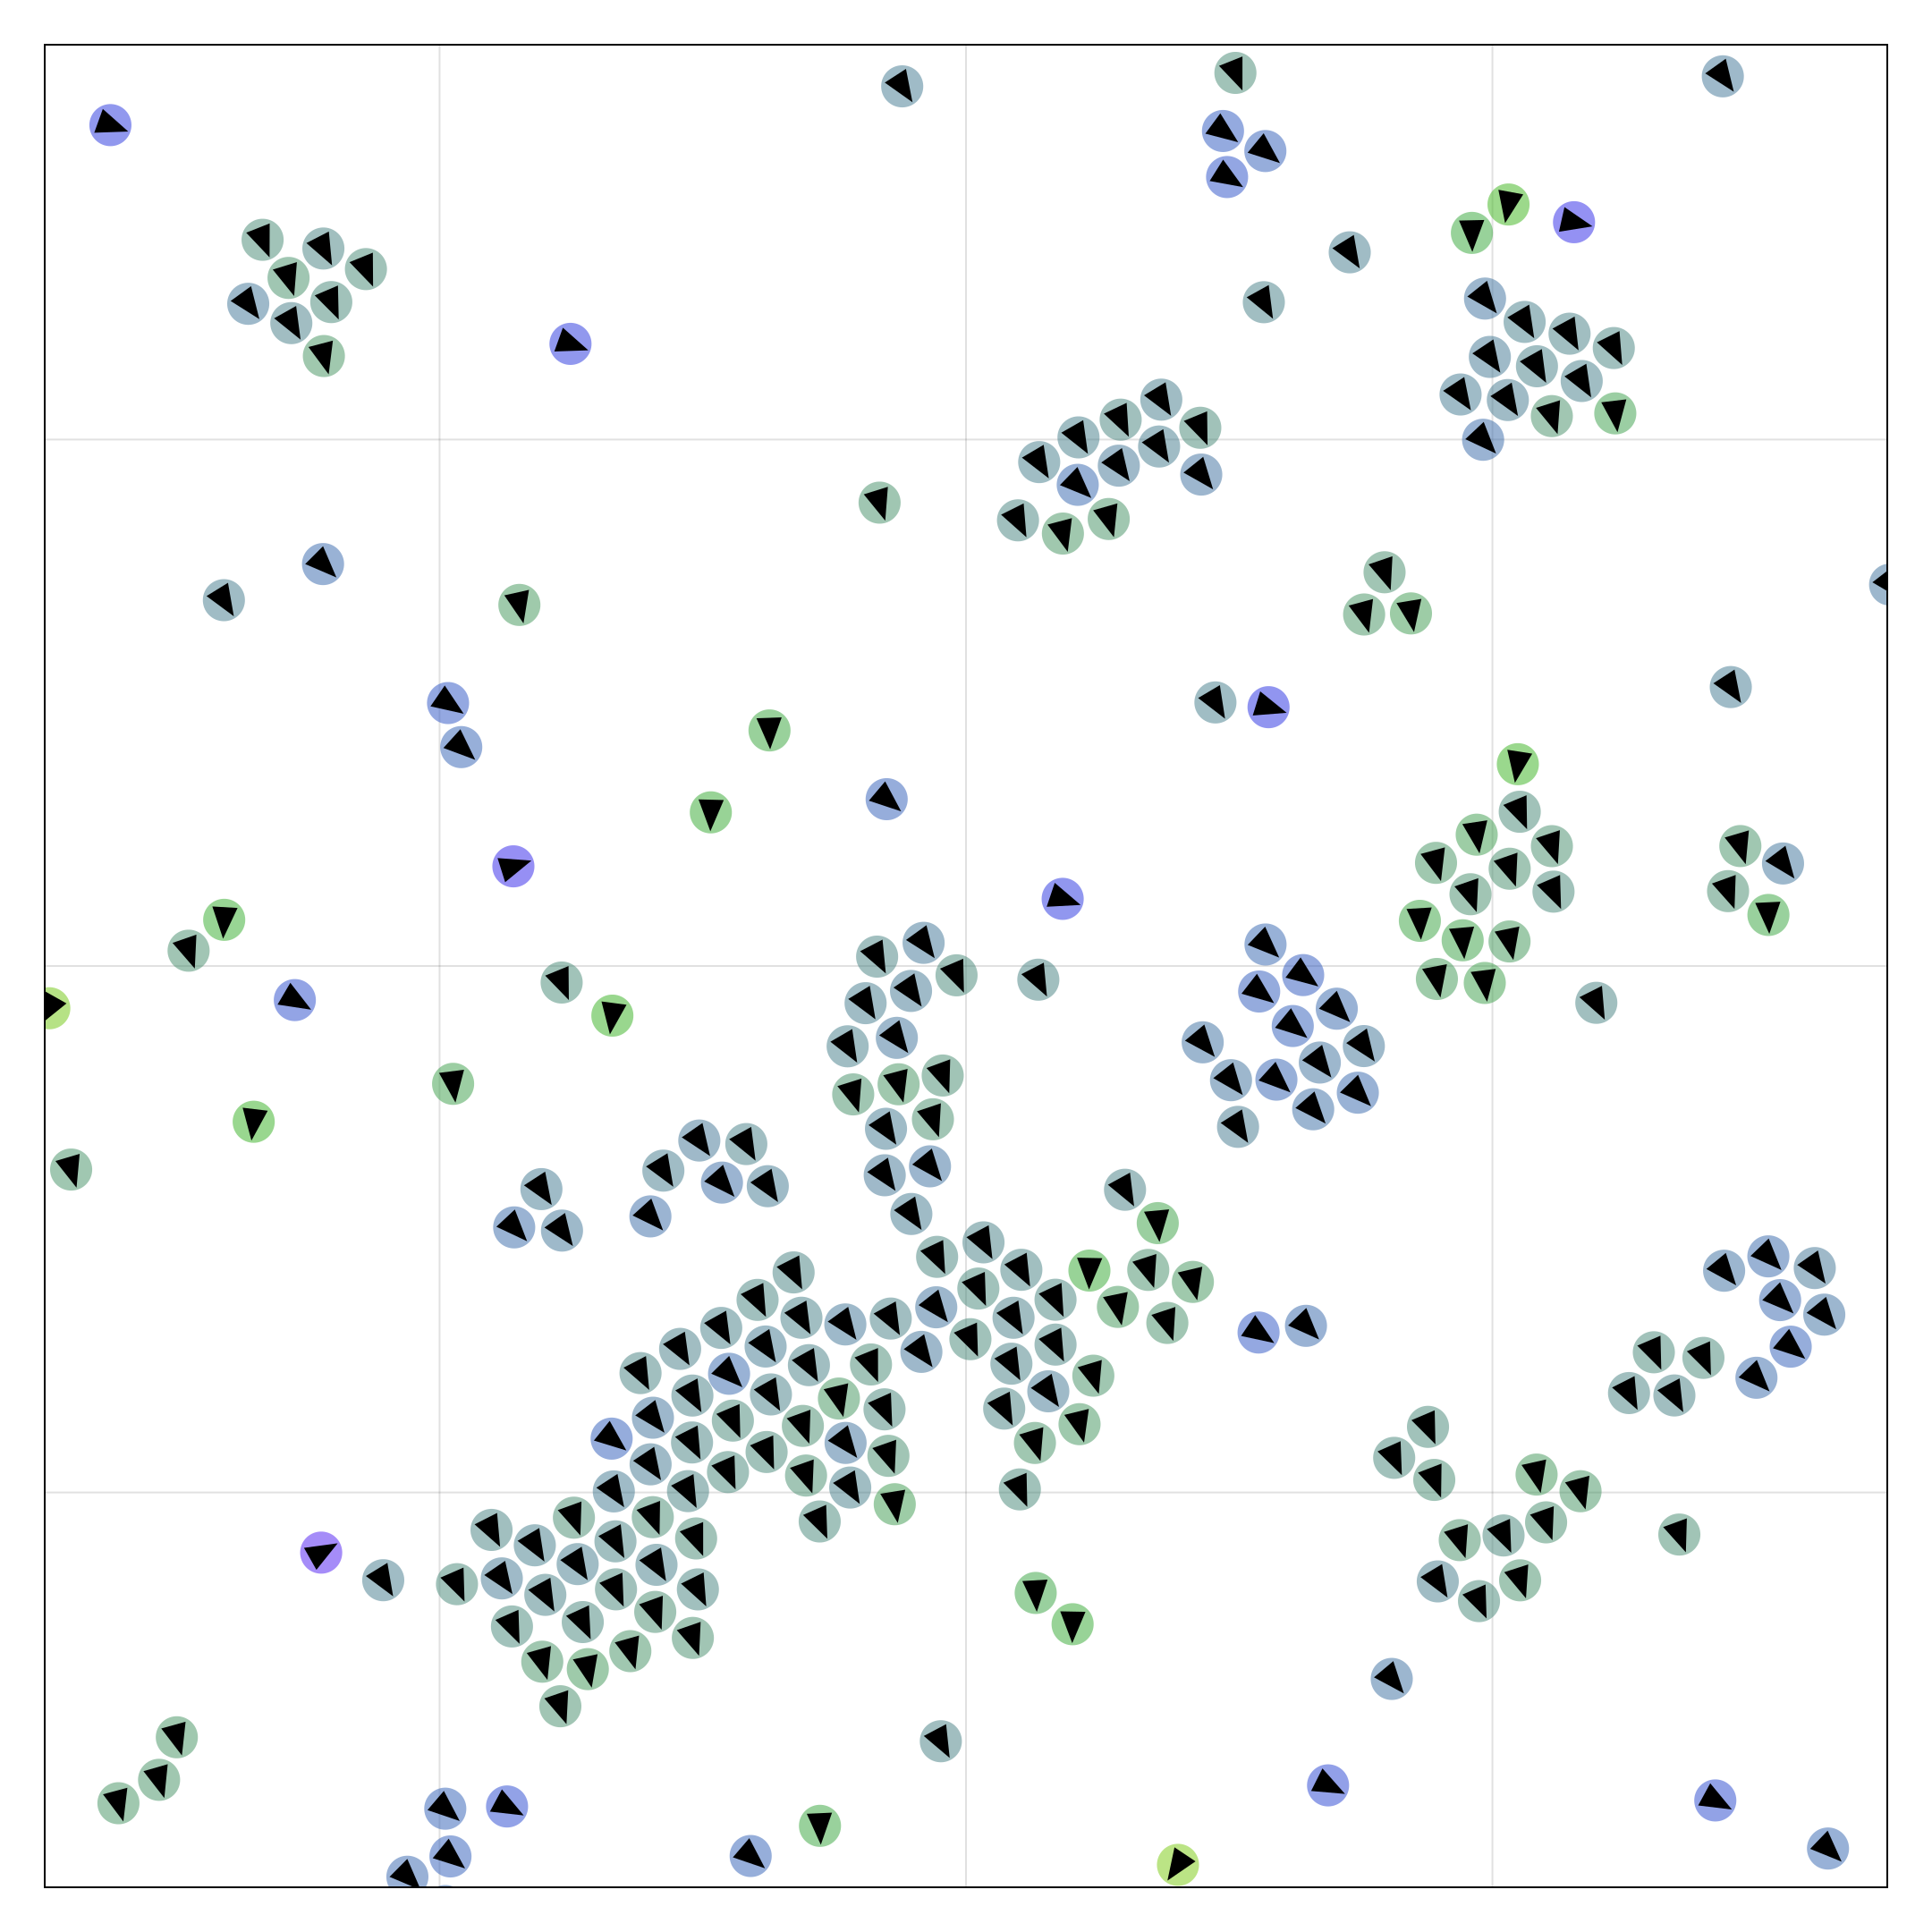
\includegraphics[width=.5\textwidth]{lj_oc/situa0.25.png}}
			\subfloat[][]{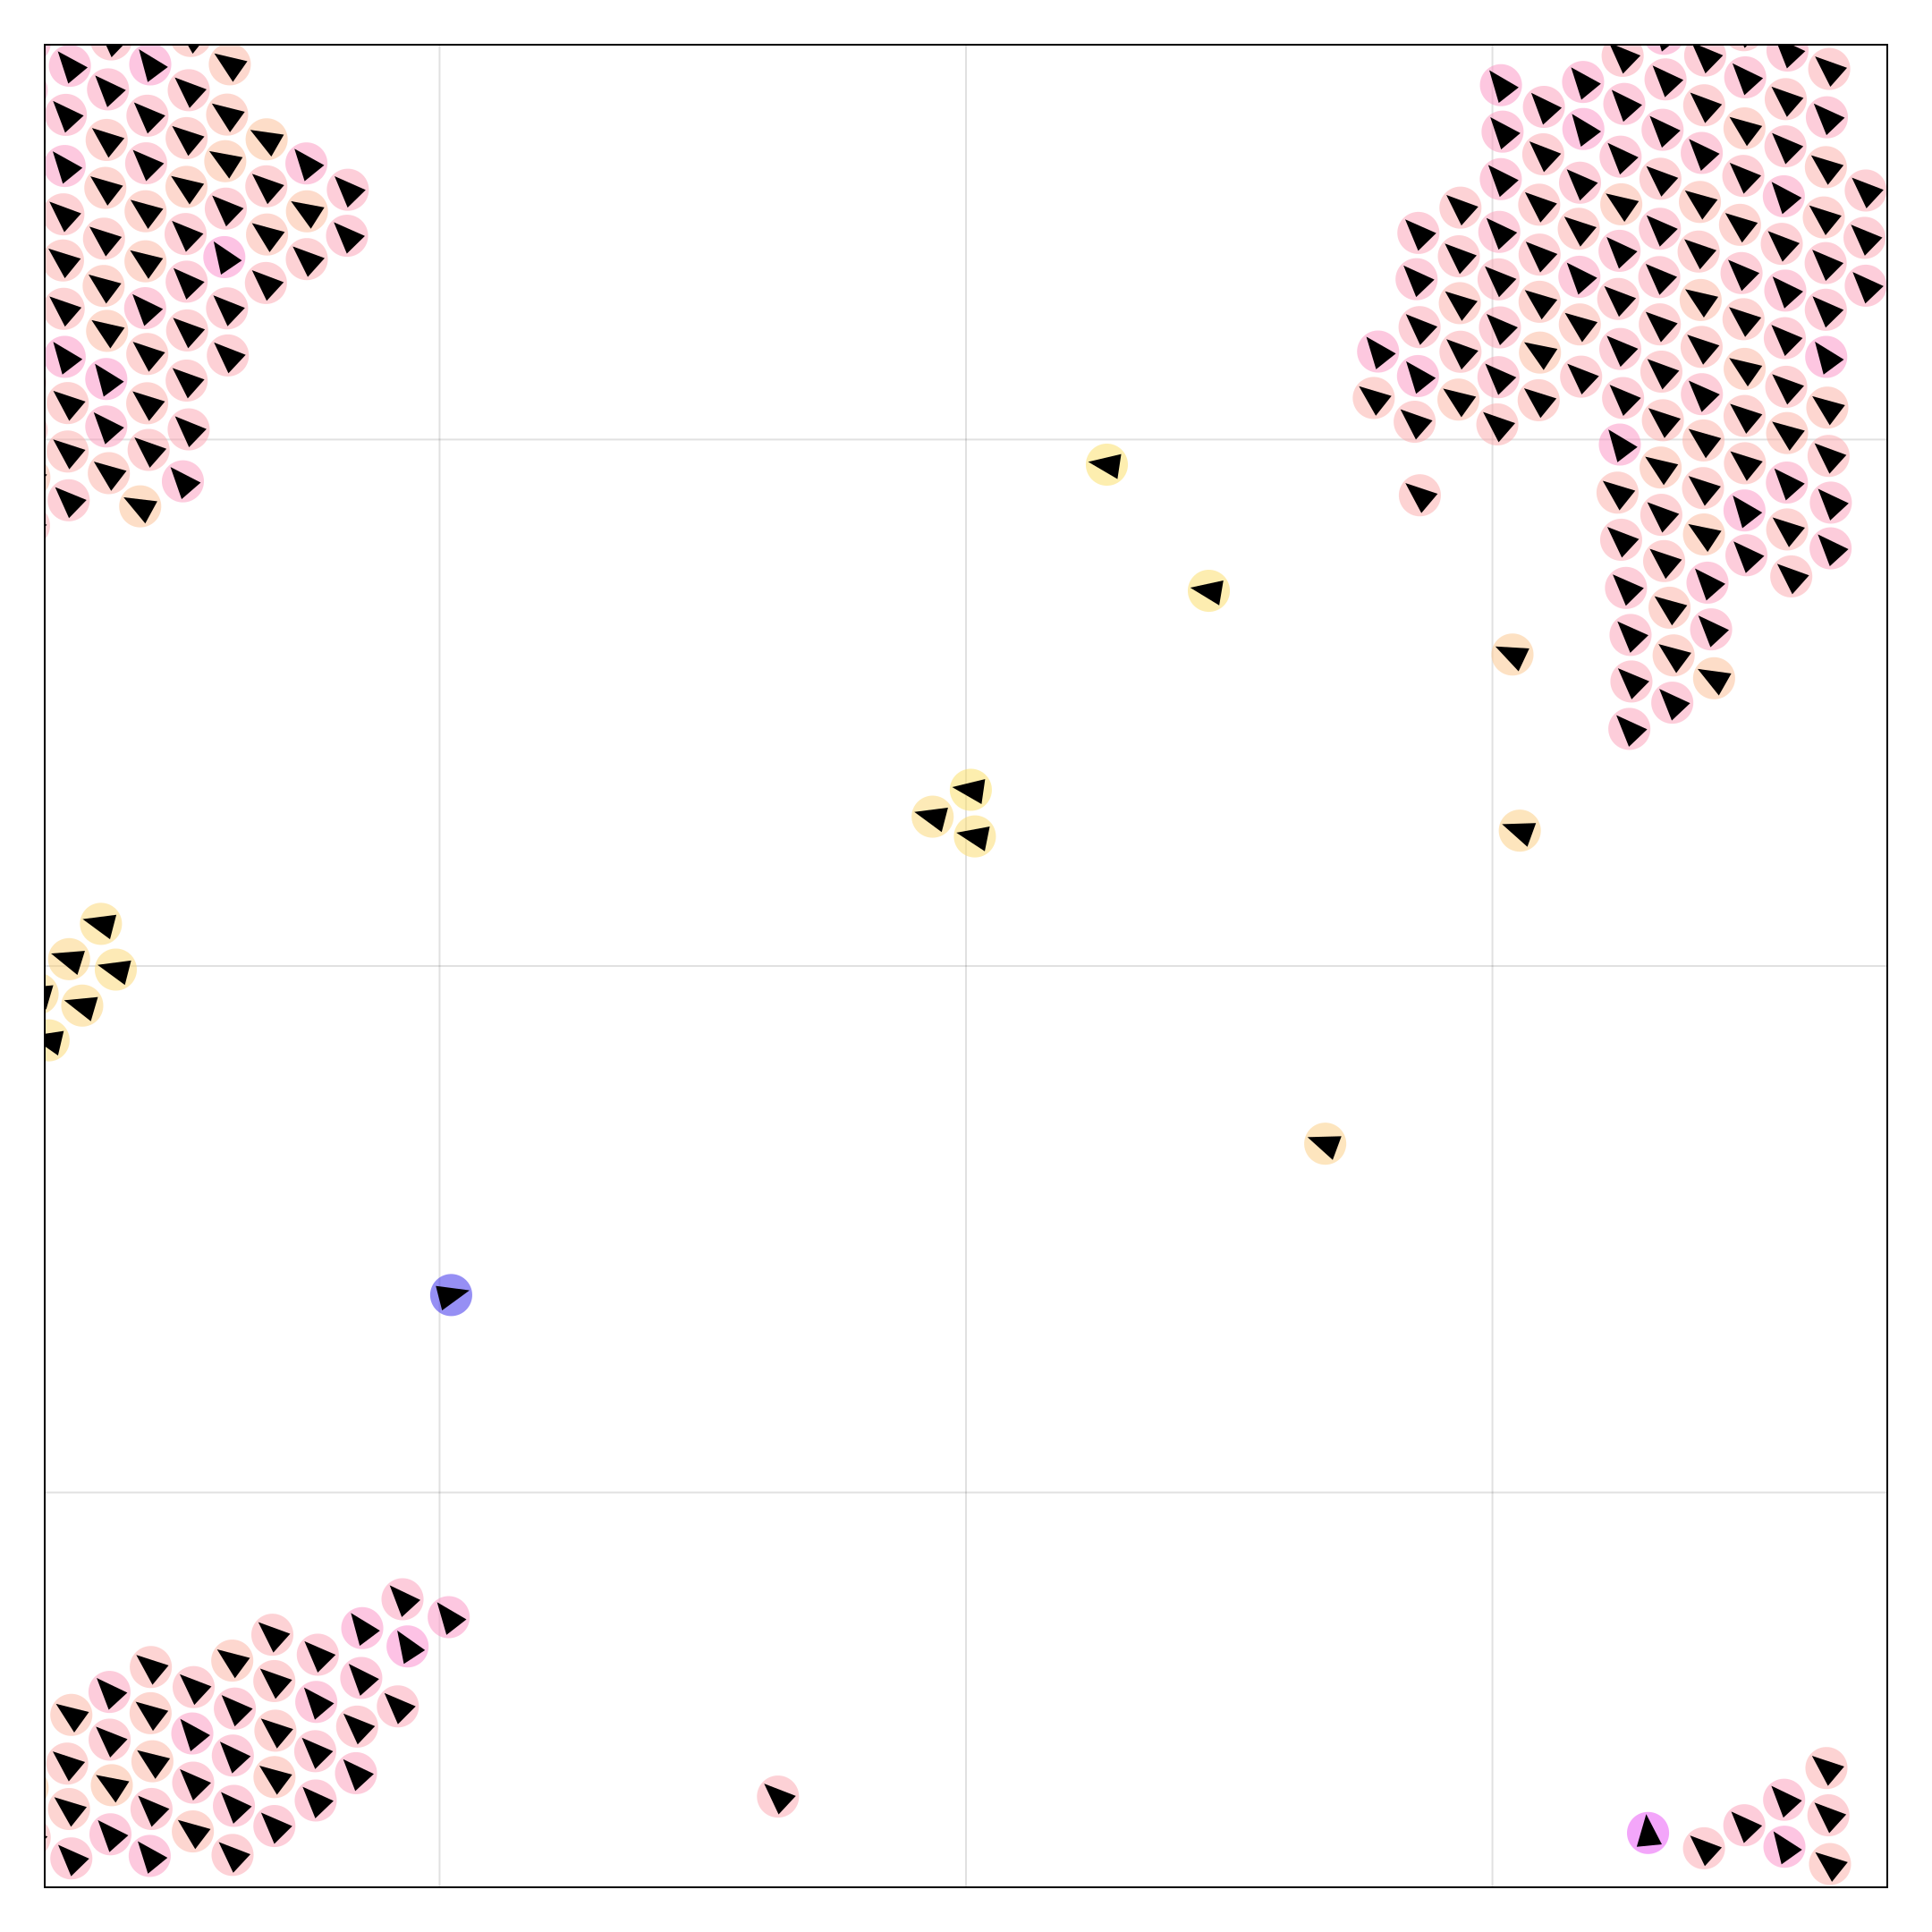
\includegraphics[width=.5\textwidth]{lj_oc/situa0.5.png}}\\
			%\captionsetup{list=false}
			\caption[]{}
		\end{figure}
		\begin{figure}[t]
			\centering
			\ContinuedFloat
			\subfloat[][]{\includegraphics[width=.5\textwidth]{lj_oc/situa0.75.png}}
			
			\caption{(continued) Representative simulation snapshots corresponding to values of off center parameter $\alpha$: (a) $\alpha = -0.75$, (b) $\alpha = -0.5$, (c) $\alpha = -0.25$, (d) $\alpha = 0$, (e) $\alpha = 0.25$, (f) $\alpha = 0.5$, (g) $\alpha = 0.75$}
			\label{fig:lj_oc_situa}
		\end{figure}
		%\todo{Situa: riunire figura}
		
		\begin{figure}[hbtp]
			\centering\
			\subfloat[][]{\includegraphics[width=.9\textwidth]{lj_oc/polar-0.75.png}}\\
			\subfloat[][]{\includegraphics[width=.9\textwidth]{lj_oc/polar-0.5.png}}\\
			\subfloat[][]{\includegraphics[width=.9\textwidth]{lj_oc/polar-0.25.png}}
			%\captionsetup{list=false}
			\caption[]{}
		\end{figure}
		\begin{figure}[hbtp]
			\ContinuedFloat
			\centering
			\subfloat[][]{\includegraphics[width=.9\textwidth]{lj_oc/polar0.0.png}}\\
			\subfloat[][]{\includegraphics[width=.9\textwidth]{lj_oc/polar0.25.png}}\\
			\subfloat[][]{\includegraphics[width=.9\textwidth]{lj_oc/polar0.5.png}}\\
			\caption[]{(continued)}
		\end{figure}
		
		\begin{figure}[t]
			\ContinuedFloat
			\centering
			
			\subfloat[][]{\includegraphics[width=.9\textwidth]{lj_oc/polar0.75.png}}
			
			\caption{(continued) Local (blue) and global (green) polarization for corresponding to values of off center parameter $\alpha$: (a) $\alpha = -0.75$, (b) $\alpha = -0.5$, (c) $\alpha = -0.25$, (d) $\alpha = 0$, (e) $\alpha = 0.25$, (f) $\alpha = 0.5$, (g) $\alpha = 0.75$}
			\label{fig:lj_oc_pol}
		\end{figure}
		%\todo{Polarizzazione: uniforma assi y dei subplot (limite 1); riunire figura}
		
		\begin{figure}[hbtp]
			\centering\
			\subfloat[][]{\includegraphics[width=.9\textwidth]{lj_oc/cluster-0.75.png}}\\
			\subfloat[][]{\includegraphics[width=.9\textwidth]{lj_oc/cluster-0.5.png}}\\
			\subfloat[][]{\includegraphics[width=.9\textwidth]{lj_oc/cluster-0.25.png}}\\
			%\captionsetup{list=false}
			\caption[]{}
		\end{figure}
			\begin{figure}[hbtp]
				\ContinuedFloat
				\centering
			\subfloat[][]{\includegraphics[width=.9\textwidth]{lj_oc/cluster0.0.png}}\\
			\subfloat[][]{\includegraphics[width=.9\textwidth]{lj_oc/cluster0.25.png}}\\
			\subfloat[][]{\includegraphics[width=.9\textwidth]{lj_oc/cluster0.5.png}}\\
			%\captionsetup{list=false}
			\caption[]{}
			\end{figure}
			\begin{figure}[t]
				\ContinuedFloat
				\centering
			\subfloat[][]{\includegraphics[width=.9\textwidth]{lj_oc/cluster0.75.png}}
			
			\caption{Maximum cluster size and cluster number corresponding to values of off center parameter $\alpha$: (a) $\alpha = -0.75$, (b) $\alpha = -0.5$, (c) $\alpha = -0.25$, (d) $\alpha = 0$, (e) $\alpha = 0.25$, (f) $\alpha = 0.5$, (g) $\alpha = 0.75$}
			\label{fig:lj_oc_clust}
		\end{figure}
		%\todo{Cluster: uniforma assi y dei subplot (sembrano leggermente diversi); riunire figura}
		
		\begin{figure}[hbtp]
			\centering\
			\subfloat[][]{\includegraphics[width=.9\textwidth]{lj_oc/rdf-0.75.png}}\\
			\subfloat[][]{\includegraphics[width=.9\textwidth]{lj_oc/rdf-0.5.png}}\\
			\subfloat[][]{\includegraphics[width=.9\textwidth]{lj_oc/rdf-0.25.png}}
			\caption[]{(continued)}
		\end{figure}
		\begin{figure}\ContinuedFloat
			\centering
			\subfloat[][]{\includegraphics[width=.9\textwidth]{lj_oc/rdf0.0.png}}\\
			\subfloat[][]{\includegraphics[width=.9\textwidth]{lj_oc/rdf0.25.png}}\\
			\subfloat[][]{\includegraphics[width=.9\textwidth]{lj_oc/rdf0.5.png}}\\
			\caption[]{(continued)}
		\end{figure}
		\begin{figure}\ContinuedFloat
			\centering
			\subfloat[][]{\includegraphics[width=.9\textwidth]{lj_oc/rdf0.75.png}}
			
			\caption{(continued) Radial distribution function at last instant of simulation corresponding to values of off center parameter $\alpha$: (a) $\alpha = -0.75$, (b) $\alpha = -0.5$, (c) $\alpha = -0.25$, (d) $\alpha = 0$, (e) $\alpha = 0.25$, (f) $\alpha = 0.5$, (g) $\alpha = 0.75$}
			\label{fig:lj_oc_rdf}
		\end{figure}
		
		\subsection{Angular Velocity}
		Simulations relative to this section are performed with a Lennard Jones strength parameter of $\epsilon = \SI{0.25}{\pico\joule}$, off centered with $\alpha = 0.5$.
		The influence of rotational self propulsion was studied generating particles' angular velocity from a normal distribution.
		To avoid inserting a bias in the system the mean is kept fixed at \SI{0}{\radian\per\second}, while changing the standard deviation in \qtylist{0.5; 1;2}{\radian\per\second}.
		This simulations tend to be less stable than ones without angular velocity, thus we needed to decrease the integration step to \SI{2.5 e-3}{\second}.
		
		With a \SI{0.5}{\radian\per\second} standard deviation, global polarization is strongly hindered, with large oscillations, though still showing an increasing trend.
		Still, local polarization remains above baseline.
		Cluster size presents an increasing trend as well, and probably a longer simulation is needed to reach steady state.
		Some peaks are still present in radial distribution function, a sign that some order is preserved in the system, at least at short and medium range.
		
		A standard deviation of \SI{1}{\radian\per\second} destroys global orientational order almost completely, while local polarization is just above the initial value.
		Situation plot in panel (b) of Figure \ref{fig:lj_av_situa} shows a system with relatively small oriented clusters; as a consequence, $g(r)$ peaks are lower than before and in a much smaller number.
		Analyzing clusters' dynamics in simulation videos, we can state that the aligning interaction, along with a nonzero angular velocity, results in small polarized clusters where particles rotate in phase around their axis.
		
		Further broadening the angular velocity distribution makes it impossible for the ensemble to develop long range order, as $g(r)$ shows.
		Polarization is completely hindered as well, both locally and globally, as graphs and situation plots show (Figures \ref{fig:lj_av_pol} and \ref{fig:lj_av_situa}).
		%\todo{uniforma assi y all'interno di ogni figura}
		\begin{figure}[hbtp]
			\centering\
			\subfloat[][]{\includegraphics[width=.5\textwidth]{lj_av/situa0.0.png}}
			\subfloat[][]{\includegraphics[width=.5\textwidth]{lj_av/situa0.5.png}}\\
			\subfloat[][]{\includegraphics[width=.5\textwidth]{lj_av/situa1.0.png}}
			\subfloat[][]{\includegraphics[width=.5\textwidth]{lj_av/situa2.0.png}}\\
			
			\caption{Representative simulation snapshots for a normal angular velocity distribution with $\mu = \SI{0}{\um\per\second}$ and standard deviation: (a) $\sigma = \SI{0}{\um\per\second}$, (b) $\sigma = \SI{0.5}{\um\per\second}$, (c) $\sigma = \SI{1}{\um\per\second}$, (d) $\sigma = \SI{2}{\um\per\second}$}
			\label{fig:lj_av_situa}
		\end{figure}
		
		\begin{figure}[hbtp]
			\centering\
			\subfloat[][]{\includegraphics[width=.9\textwidth]{lj_av/polar0.0.png}}\\
			\subfloat[][]{\includegraphics[width=.9\textwidth]{lj_av/polar0.5.png}}\\
			\subfloat[][]{\includegraphics[width=.9\textwidth]{lj_av/polar1.0.png}}
			%\captionsetup{list=false}
			\caption[]{}
		\end{figure}
		\begin{figure}
		\centering
		\ContinuedFloat
			\subfloat[][]{\includegraphics[width=.9\textwidth]{lj_av/polar2.0.png}}\\
			
			\caption{(continued) Local (blue) and global (green) polarization for a normal angular velocity distribution with $\mu = \SI{0}{\um\per\second}$ and standard deviation: (a) $\sigma = \SI{0}{\um\per\second}$, (b) $\sigma = \SI{0.5}{\um\per\second}$, (c) $\sigma = \SI{1}{\um\per\second}$, (d) $\sigma = \SI{2}{\um\per\second}$}
			\label{fig:lj_av_pol}
		\end{figure}
		
		\begin{figure}[hbtp]
			\centering\
			\subfloat[][]{\includegraphics[width=.9\textwidth]{lj_av/cluster0.0.png}}\\
			\subfloat[][]{\includegraphics[width=.9\textwidth]{lj_av/cluster0.5.png}}\\
			\subfloat[][]{\includegraphics[width=.9\textwidth]{lj_av/cluster1.0.png}}
			%\captionsetup{list=false}
			\caption[]{}
		\end{figure}
		\begin{figure}
		\centering
		\ContinuedFloat
			\subfloat[][]{\includegraphics[width=.9\textwidth]{lj_av/cluster2.0.png}}\\
			
			\caption{(continued) Maximum cluster size and cluster number for a normal angular velocity distribution with $\mu = \SI{0}{\um\per\second}$ and standard deviation: (a) $\sigma = \SI{0}{\um\per\second}$, (b) $\sigma = \SI{0.5}{\um\per\second}$, (c) $\sigma = \SI{1}{\um\per\second}$, (d) $\sigma = \SI{2}{\um\per\second}$}
			\label{fig:lj_av_clust}
		\end{figure}
		
		\begin{figure}[hbtp]
			\centering\
			\subfloat[][]{\includegraphics[width=.9\textwidth]{lj_av/rdf0.0.png}}\\
			\subfloat[][]{\includegraphics[width=.9\textwidth]{lj_av/rdf0.5.png}}\\
			\subfloat[][]{\includegraphics[width=.9\textwidth]{lj_av/rdf1.0.png}}
			%\captionsetup{list=false}
			\caption[]{}
		\end{figure}
		\begin{figure}[t]
		\centering
		\ContinuedFloat
			\subfloat[][]{\includegraphics[width=.9\textwidth]{lj_av/rdf2.0.png}}\\
			
			\caption{(continued)Radial distribution function at last instant of simulation for a normal angular velocity distribution with $\mu = \SI{0}{\um\per\second}$ and standard deviation: (a) $\sigma = \SI{0}{\um\per\second}$, (b) $\sigma = \SI{0.5}{\um\per\second}$, (c) $\sigma = \SI{1}{\um\per\second}$, (d) $\sigma = \SI{2}{\um\per\second}$}
			\label{fig:lj_av_rdf}
		\end{figure}
		
    \section{Conclusions to chapter 3}
    \label{3concl}
    Along this chapter we studied how our model can be used in a theoretical investigation of both phase transitions and collective behaviors.
    We showed that, without an explicitly aligning torque, our system undergoes a flocking transition, similar to what happens with original or continuous Vicsek models that have been built for that purpose.
    Such a phenomenon can be efficiently studied as a continuous phase transition, where the order parameter shows the expected behavior.
    The similarities between this model and the one studied in \cite{martin-gomez_collective_2018} suggests that these aligning particles systems could be part of the same universality class, but more investigation is needed in those regards.
    
    Regarding the effect of simulation features on collective behaviors we showed that, in general, adding more complexity with some angular or linear velocity distribution tends to disrupt long range order in positions, while the presence of larger velocities (both in the case of one velocity and distributions) has the tendency to align the system, with faster particles spreading information across the board.
    In general, positional and orientational order are related when the same velocity is applied to all particles and a clustered system is a flocking system in most cases, while we showed how different velocities can still result in an aligned, although not clustered, system.
    
    All the macroscopic behaviors, such as clustering and flocking, showed here are not observed during experiments in the host lab.
    This could be due to weak or short-range interactions, as well as more complex effect involving the solvent.
    
    
    We can conclude that the suite of tools we developed offer a fast and efficient way to study at least some of the collective behaviors featured in a systems like the one we are interested in.
    In principle, adapting these tools to analyze experimental videos of tracked particles will not be hard due to their implementation and will possibly lead to a better study of the quantitative correspondence between simulated and experimental active particles, to deepen what was started with the qualitative agreement in \ref{qualitative}.
    Nonetheless, in the experiments like the ones held in Microscale Robotics Lab, it is hard to work with high packing fraction, since the \ch{2 H2O2 ->[Pt] 2 H2O + O2} reaction that propels particles tend to produce \ch{O2} bubbles that disturb observation: higher packing fraction means more bubbles, making the system difficult to observe.
    While this thesis gets written, experimentation with \ch{Cu} particles is ongoing, and the observations suggest that said particles produce few or no bubbles, making them a more suitable case study for high packing fraction situations.
    As snapshots in \ref{qualitative} show, measuring the orientation of observed particles is not a straightforward task, since the boundary between the two hemispheres is not always clearly observable.
    This will make harder to apply the polarization measurements to experimental videos. 
    The fact that observed system show only local clustering and no flocking make us predict that the most useful tools among the ones developed in this work will be the local-focused ones, especially the cluster size measurement, which is the immediately applicable one for experimental situations.

    \end{document}